

%\documentclass{sig-alternate-10pt}
%\documentclass[10pt,nocopyrightspace,preprint]{sigplan-proc-varsize}

\documentclass[journal]{IEEEtran}
%% INFOCOM 2011 addition: 

\makeatletter
\def\ps@headings{%
%\def\@oddhead{\mbox{}\scriptsize\rightmark \hfil \thepage}%
%\def\@evenhead{\scriptsize\thepage \hfil \leftmark\mbox{}}%
%\def\@oddfoot{}%
%\def\@evenfoot{}}

\def\@oddhead{}%
\def\@evenhead{}%
\def\@oddfoot{\hfil \thepage \hfil}%
\def\@evenfoot{\hfil \thepage \hfil}}

\makeatother
%\pagestyle{headings}

%\documentclass[10pt,nocopyrightspace,preprint]{sigplan-proc-varsize}

\usepackage{subfigure, verbatim, soul}
\usepackage{comment,pifont,array,url,amsmath,multirow,latexsym,tabularx}
\usepackage{ifpdf,rotating,colortbl}
\usepackage{graphicx}
\usepackage[boxed]{algorithm}
\usepackage{algorithmic}
\usepackage{xspace}
\usepackage{url}
\usepackage{bbm}
\usepackage{wrapfig}

\newcommand{\eat}[1]{}


\title{Beyond MLU: An Application-Centric Comparison of Traffic Engineering Schemes}

\date{}
%\numberofauthors{1} 
%\author{\alignauthor Abhigyan Sharma,Aditya Mishra,Vikas Kumar, Arun Venkataramani \\
%\affaddr{Dept. of Computer Science, University of Massachusetts} \\ \affaddr{ Amherst, MA, USA} \\
%\email{abhigyan@cs.umass.edu, adityam@cs.umass.edu,vikas@cs.umass.edu,arun@cs.umass.edu}
%}

\author{Abhigyan Sharma, Aditya Mishra, Vikas Kumar, Arun Venkataramani%
\thanks{The authors are with the Department of Computer Science, University of Massachusetts, Amherst, MA 01003 USA (e-mail: abhigyan@cs.umass.edu; vikas@cs.umass.edu; adityam@cs.umass.edu; arun@cs.umass.edu)}% <-this % stops a space
\thanks{Manuscript received Oct 27, 2012.}}%


%\author{\IEEEauthorblockN{Abhigyan Sharma, Aditya Mishra, Vikas Kumar, Arun Venkataramani}
%\IEEEauthorblockA{Dept. of Computer Science, University of Massachusetts Amherst}
%}

%\author{Abhigyan Sharma,Aditya Mishra,Vikas Kumar, Arun Venkataramani}
%\affiliation{University of Massachusetts Amherst}


%\markboth{Journal of \LaTeX\ Class Files,~Vol.~6, No.~1, January~2007}%
%{Shell \MakeLowercase{\textit{et al.}}: Bare Demo of IEEEtran.cls for Journals}

%\Email{abhigyan,adityam,vikas,arun,@cs.umass.edu}
%\usepackage{geometry} 
%\usepackage{amsmath}    % need for subequations
%\usepackage{amssymb}
%%\usepackage[pdftex]{graphicx}
%\usepackage{subfigure}
%\usepackage{marvosym}
%\geometry{left=1.0in,right=1.0in,top=1in,bottom=1in}

%\newcommand{\tbd}[1]{\footnote{[{\bf{#1}}]}}
\newcommand{\tbd}[1]{}

\newcommand{\opt} {Optimal}
\newcommand{\mplsavg} {MPLS}
\newcommand{\invcap} {InvCap}
\newcommand{\optwt} {OptWt}
\newcommand{\cope} {COPE}
\newcommand{\mindelay} {MinDelay}

\newcommand{\CAP} {SPF}
\newcommand{\maxiodiff} {Max-IO-Diff}

\begin{document}

\maketitle

%!TEX root = New.tex
\begin{abstract}

Many datacenters are primarily used for content delivery. These datacenters are typically lightly loaded during normal operation, and hence have significant potential for saving energy. However, saving energy by shutting off servers could reduce cache-hit rates and by shutting off network components could increase datacenter network congestion; both events hurt user-experience. Due to these perceived risks, operators leave entire datacenters in an always on state foregoing all energy savings.

Towards the goal of saving energy in data center networks, we present \shrink, a cluster manager that makes power management decisions for networks and servers in a coordinated manner  to maximize energy savings, and  decides load balancing and traffic engineering  to ensure a minimal impact on user-perceived performance.
Further, \shrink\ orchestrates content transfers before server shutdown events to minimize the impact of server shutdown on cache hit rates.  We implement a prototype of \shrink\ using \TBD{TBD} library, and conduct extensive trace-driven evaluation using traces from a large CDN. Our results show that \shrink\ can reduce energy consumption by TBD-TBD\% with minimal impact on user-perceived performance and saves energy within TBD\% of the optimal strategy.

\end{abstract}

\begin{IEEEkeywords}
Computer network management,  cost function, IP networks, optimization, routing.
\end{IEEEkeywords}


\chapter{Traffic Engineering: An Application-Centric Comparison}
\label{ch:beyondmlu}

\section{Introduction}

\subsection{Shortcomings of link utilization metrics}

\subsection{Challenges in evaluating TE schemes}

\subsection{Results from an application-centric evaluation}

\subsection{Chapter organization}

Traditionally, traffic engineering (TE) has been studied as an optimization problem that takes as input a traffic matrix (TM) and seeks to compute routes so as to minimize a network cost function. The cost function is intended to capture the severity of congestion hotpsots based on link utilization levels. For example, the most widely used cost function, MLU, is simply the utilization of the most utilized link in the network \cite{COPE,TEXCP,MultiTM,Cohen}; others  sum over all links a convex function of their utilization  (so as to penalize highly utilized links more)  \cite{fortz2000internet,fortz2002traffic}. There are two implicit assumptions underlying this line of work. First, maintaining low link utilization improves user-perceived application performance under typical load conditions. Second, maintaining low link utilization increases the effective capacity of the network by enabling it to accommodate unexpected surges in the traffic demand.

Our work questions both of the above assumptions. The distinguishing aspect of our work is an application-centric approach to the problem: instead of posing TE as as optimization problem seeking to minimize link utilization, we focus on application performance metrics such as TCP throughput for elastic  traffic and quality-of-service metrics (e.g., MOS score for VoIP quality \cite{MOS-formula}) for inelastic traffic. Accordingly, our evaluation methodology is empirical: instead of relying on mathematical simulations based on linear programming or heuristic techniques for NP-complete problems, our experiments carefully and at scale simulate end-to-end application behavior so as to compare TE schemes with respect to their impact on application performance. 

Our application-centric and empirical approach reveals rather unexpected results. Our first finding is that metrics based on link utilization alone, and in particular MLU, are a poor proxy for application performance. For example, a TE scheme may incur twice the MLU of another TE scheme and yet achieve as good or better application performance. The key reason for this mismatch is that application performance is largely determined by end-to-end loss rate and delay, but link utilization does not capture them accurately. At typical Internet loads, and in fact until the utilization starts approaching the capacity, link loss rates remain negligibly small. This observation has also been confirmed by explicit measurements on Internet backbones \cite{ExpRouterBuffer}, and is consistent with studies on ISP backbones showing that over 90\% of all packet loss is caused by interdomain routing fluctuations as opposed to high utilization \cite{SprintStudy} and 90\% of TCP flows experience no packet loss \cite{SprintBackbone}. Furthermore, end-to-end Internet path delays are known to be largely determined by propagation delays as opposed to queueing delays \cite{SprintBackbone,SingleHopDelay}. 

As a result, we find that all state-of-the-art TE schemes achieve nearly identical application performance at typical Internet load levels. In fact, even static shortest-path routing with link weights inversely proportional to the capacity (\invcap) (i.e., no engineering at all) achieves the same application performance as optimal TE. Ironically, TE schemes that engineer for unexpected traffic spikes (e.g., COPE \cite{COPE}) consistently hurt TCP throughput despite achieving near-optimal MLU.

More surprisingly, we find that application adaptation to location diversity,  i.e., the ability to download content from multiple potential locations, blurs differences even in the achieved capacities of different TE schemes enabling all of them to be near-optimal. With location diversity, we find that the inverse of the MLU is no longer a meaningful metric of capacity. Instead, we formalize a new metric of the capacity achieved by a TE scheme called the {\em surge protection factor} (SPF) that captures the factor of increase in demand that can be sustained while accounting for location diversity. TE schemes calculate routing based on a measured traffic matrix to achieve a desired network cost, but application adaptation to location diversity changes the traffic matrix itself in response to a change in routing resulting a different network cost than expected. As a result, the optimal TE scheme with perfect knowledge of traffic matrix and sub-optimal TE schemes like OSPF weight-tuning \cite{fortz2000internet} end-up achieving the same SPF. Even the static routing scheme, \invcap, achieves an SPF at most 30\% worse than optimal TE.


The rest of the chapter is as follows. Section \ref{sec:locdiv-background} explains how location diversity changes the TE problem. Section \ref{sec:exp_setup} presents our simulation setup. Section \ref{sec:app_performance} compares the application performance of TE schemes and Section \ref{sec:capacity} compares their achieved capacity under location diversity. 


\section{Engineering traffic with location diversity}
\label{sec:locdiv-background}

This section introduces location diversity and proposes a new metric to quantify the capacity achieved by traffic engineering schemes with location diversity.


\subsection{Location diversity: Prevalence}

Location diversity, or the ability to download content from multiple potential locations, is widespread in the Internet today. Major commercial CDNs, e.g., Akamai \cite{Akamai}, Level-3 \cite{Level-3}, EdgeCast \cite{edgecast} etc., commonly replicate content at hundreds of locations and redirect users to the best server based on proximity or dynamic monitoring of server and network congestion \cite{akamai-detour}. Popular P2P applications such as BitTorrent \cite{bittorrentprotocol}, PPLive \cite{PPLive} download content simultaneously from many peers that are chosen based on a number of factors including network congestion. Other examples of location diversity include cloud computing infrastructure providers such as Google and Amazon with geographically distributed sites; content hosting services such as Carpathia \cite{Carpathia}, Rapidshare \cite{OneClickHosting}, etc.; mirrored websites such as SourceForge, Debian, etc. 


Although quantifying the extent of location diversity in today's Internet is difficult, back-of-the-envelope calculations based on existing measurement studies suggests that it is significant.  CDNs alone are estimated to account for 10\% of Internet traffic \cite{AtlasReport}. Major cloud computing and content hosting companies with location diversity contribute to a significant fraction of Internet traffic, e.g., Google (6\%), Comcast (3\%), RapidShare (5\%) and Carpathia (0.5\%), a trend that is projected to increase in the near future \cite{urlinternet,AtlasReport}. The fraction of P2P traffic in Internet was estimated to be between 18-60\% by different measurement studies in 2009.  


\subsection{Location diversity: Quantifying capacity}

How can we quantify the capacity achieved by a TE scheme in the presence of location diversity? In general, the capacity is a {\em region} that includes all of the traffic matrices that it can accommodate. However, quantifying the capacity of a TE scheme as a region may shed little light on its ability to tolerate typically encountered load spikes. Furthermore, it is cumbersome to compare TE schemes that achieve overlapping capacity regions. So, it is common to use a more concise metric such as the MLU to characterize the capacity with respect to a given traffic matrix. Intuitively, the inverse of the MLU serves as a metric of capacity, e.g., if a TE scheme achieves an MLU of 0.25 for a given matrix, then it can tolerate up to a 4$\times$ surge in the load represented by the matrix. Unfortunately, MLU is not a meaningful metric of capacity when application adaptation to location diversity  determines the traffic matrix (Chapter \ref{ch:te-background},  Section \ref{sec:bg-3node}).
  

With location diversity, the demand is best represented as a ``content matrix'' that specifies for each node and each content the traffic for that content at that node and the set of source locations from where that content can be downloaded. The traffic matrix corresponding to this demand depends upon the underlying routes and application behavior (e.g., how parallel TCP splits traffic across the download locations). Furthermore, scaling the demand does not simply scale the traffic matrix entries by the same factor. In general, it is difficult to predict how application behavior might change the traffic matrix for a projected surge in demand, as that change depends upon the underlying routes that in turn depend upon the original traffic matrix. Indeed, as the example in Chapter \ref{ch:te-background},  Section \ref{sec:bg-3node} shows, even if the demand is unchanged, the mere act of engineering routes can change the traffic matrix yielding a different MLU than expected.


\subsubsection{An empirical capacity measure}
\label{sec:SPFdefinition}
%\textbf{proposing a new metric}

We propose a new metric, {\em surge protection factor} (SPF), to quantify the capacity achieved by a TE scheme with respect to a traffic matrix. Let $E$ denote a TE scheme, $M$ the demand specified as a content matrix. When there is no location diversity, $M$ can be easily transformed to a unique traffic matrix $T(M)$. Let  MLU$(E,T(M))$ denote the MLU achieved by $E$ given the traffic matrix $T(M)$. In this case, SPF$(E,M)$ is simply the inverse of MLU$(E,T(M))$, i.e., the factor of increase in the demand that can be satisfied. However, in the case when there is location diversity, SPF$(E,M)$ is an {\em empirical} measure of the satisfiable increase in demand computed as follows. Let $kM$ denote the demand that scales each entry in $M$ by a factor $k>1$. Then, SPF$(E,M)$ is defined as the largest $k$ such that the routing computed by $E$ (for the matrix $T(M)$) can satisfy the demand $kM$.

Determining if an engineering scheme can satisfy a projected demand is difficult as it requires us to accurately model application adaptation to location diversity, so SPF is useful mainly as an empirically measured capacity metric. To this end, we describe our experimental setup next.

%
\section{Location diversity changes TE problem}
%Current TE model assumes a static traffc matrix but  application adaptation due to location diversity can change the traffic matrix based on congestion in network or even a change in routing in the network.
%\begin{figure}[htb]
%%\vspace{-0.3in}
% \begin{center}
%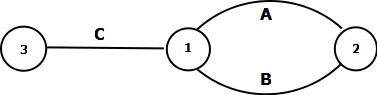
\includegraphics[scale=0.4]{final_images/Diagram3node.png}
%\end{center}
%	  \caption{Three Node Network}
%	\label{fig:3node} 
%%\vspace{0.1in}
%\end{figure}

% point: location diveristy makes TE difficult by changing TM; it is even difficult to estimate the traffic matrix after TE since 

The objective of TE is to ensure the the link utilization in the network is at minimal level but location can alter its effects by chanigng the traffic matrix and hence the utilization of links in the network.

\textbf{explain conditions}
We explain it using the three node netowrk in Figure~\ref{fig:3node}.
All link have capacity of 100 units and a constant delay.  Link A has a very small delay compared to links B and C; both B and C have equal delay. Node 1 has 100 units of demand which it can route from 2 as well as 3. In addition there is 20 units of demand at node 1 which it routes from 2. We assume that that the aggregate flow at a node constitutes of infinitesimal flows which can be split among multiple source locations. Similar to parallel TCP behavior, the ratio in which flows are split among multiple locations is inversely proportional to delay from a location. The routing in network is shortest path routing based on link weights and traffic is split equally among multiple path with equal weights.

\textbf{point: TE cannot be achieved since adaptation changes TM.}
Initially, link weights of A, B and C as 3, 2, 1 respectively. The traffic between 1 and 2 is routed only using B. 1 splits its demand of 100 units equally among 2 and 3. Thus traffic on links is A = 0, B = 70, and C = 50. In the next step, to balance load between A and B both link are set equal weights.  Let see how parallel TCP connections would change our estimates of link utilization in this case. Assuming each infinitesimal flow uses only one of the two links A and B, 50 unit of demand at 1 is routed using links B and C, and equal amount using A an C. In addition, the 20 units of background traffic is split equally among links B and C.  Since A has a much smaller delay than C, 50 units of demand at 1 routed using A and C will flow entirely through A. The demand routed using B and C will be split equally among B and C respectively. Thus traffic on links is A = 60, B = 35, and C = 25 which is different from expected values of A = 35, B = 35, C = 50. Thus, location diversity makes TE difficult by changing the traffic matrix and changing expected link utilization.

\section{Experimental setup}
\label{sec:exp_setup}

In this section, we describe our experimental setup based on ns-2 used to compare TE schemes with respect to their impact on application performance. 
We chose ns-2 as it is well-suited for simulating thousands of flows in an ISP network at the packet level while also incorporating transport and application behavior in a fine-grained manner.

% Evaluating application performance accurately necessitates modeling application and transport behavior, especially their response to network characteristics, in a fine-grained manner. We chose ns-2 as the simulation platform as it is well-suited to simulate thousands of flows in an ISP network at the packet level while also incorporating transport and application behavior in a fine-grained manner.


%Below, we discuss (1) why this simulation infrastructure is necessary, (2)  how we simulate real traffic matrices using ns-2, and (3) the traffic engineering schemes, real ISP topologies, and real traffic matrices in our experiments.

%In this section we describe our ns-2 simulation infrastructure to compare application performance for traffic engineering methods. First we discuss why this simulation infrastructure is necessary,  next we explain how we simulate traffic matrices using ns-2, and then we describe the TE schemes we compare and the ISP topologies and traffic matrices in our simulation.

%Our goal is to study the impact of TE schemes on end-to-end application performance. TE impacts application performance in several ways. First, TE determines the utilization on backbone links in the network, which in turn influences the loss rate and queuing delay of those links. Second,  TE determines the route between PoPs in the network and thereby impacts path delays. These factors---propagation delay, queuing delay, and loss rate---primarily influence user-perceived application performance, e.g., the loss rate and path delay determines TCP performance as well as the quality of streaming applications.

% Evaluating application performance accurately necessitates modeling application and transport behavior, especially their response to network characteristics, in a fine-grained manner. We chose ns-2 as the simulation platform as it is well-suited to simulate thousands of flows in an ISP network at the packet level while also incorporating fine-transport and application behavior in a fine-grained manner.


%\label{fig:ISP_data}
%\begin{wrapfigure}[12]{r}{0.25\textwidth}\footnotesize
%  \begin{center}
%  \begin{tabular}{ p{0.7cm} | p{0.7cm} | p{0.8cm}  }
%\textbf{BW (Mbps)} &\textbf{US users \%}  & \textbf{Europe users \% } \\ \hline 
%0.25 & 4.9 &   1.5 \\
%2.0  & 38.1 & 26.2  \\
%5.0 & 32.4 & 57.8	\\
%10.0 & 20.0 & 14.5 \\
%20.0 & 4.6 & - \\
%  \end{tabular}
%  \end{center}
%  \caption{Bandwidth Distribution}
%\end{wrapfigure}
%\label{fig:bandwidth_distribution}

%in order to determine link utilization levels and evaluate cost functions based on them. But, these cost functions do not capture network wide application performance.  They can be biased by traffic on one or a few links and  do not take into account the path delay which is important for application performance.  Simulation is the simplest approach to get a reasonable estimate of application performance. Another approach we considered was using theoretical model e.g. fixed point \cite{fixedpoint} models for large number of network flows. Since these are theoretical models, they do contain modeling errors. Another reason, we excluded theoretical models is these models are  not well understood  for a network with multiple bottleneck links \cite{fixedpoint}. Since we use a simulation infrastructure, our experiments are prone to simulation errors. An even more accurate experiment would involve emulation ( e.g Emulab) or a  virtualized infrastructure (e.g. VINI \cite{VINI} ) but we restricted ourselves to doing ns-2 simulations because its ease of use enabled us to run large number of experiments.



\subsection{Simulating traffic matrices in ns-2}
\label{sec:sim_TM}

Figure~\ref{fig:simulation1} illustrates the experimental process. Each simulation has three inputs: (1) \textsl{ISP Topology} (2) a sequence of \textsl{File Arrivals} at each node based on the current \textsl{TM} (3) \textsl{Routing}, as computed using a \textsl{TE} scheme. %The slanted text refers to the corresponding block in Figure~\ref{fig:simulation1}.

We construct an ISP network topology from our dataset consisting of PoP-level ISP topology maps. PoPs are represented as nodes and links between these nodes are the backbone links of the ISP. Each PoP node has a number of users connected to it via separate access links. Each PoP node also has five server nodes connected to it via high capacity links that serve files to users. The number of user nodes in our simulation ranges from 300-6000 nodes and the capacity of backbone links varies from 50Mbps to 1Gbps.

\begin{figure}
 \begin{center}
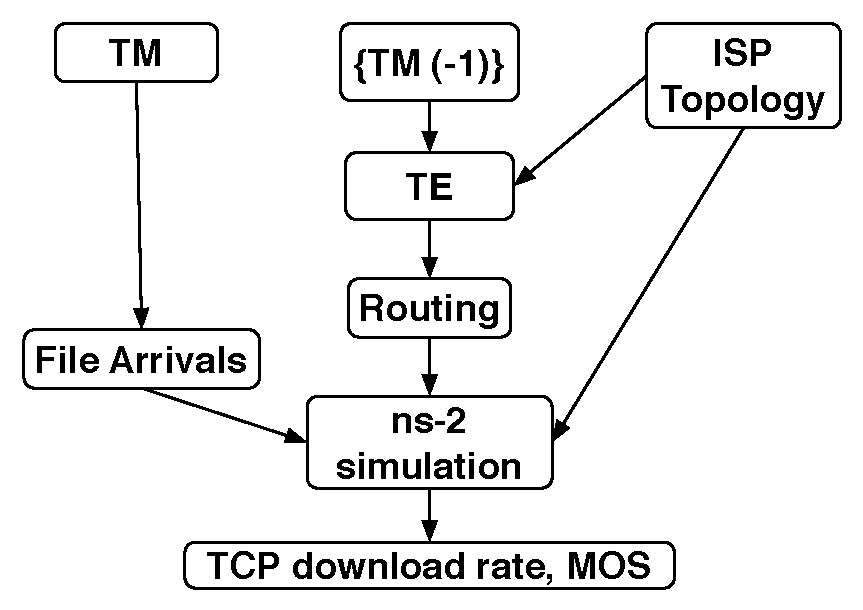
\includegraphics[scale=0.4]{final_images/Simulation1.pdf}
\caption{Block diagram of experiment process}
 \end{center}
 \label{fig:simulation1}
 \end{figure}
 
%\begin{figure}[tbh]
%  \begin{center}
%\includegraphics[scale=0.42]{}
% \end{center}
%\vspace{-0.1in}
%	  \caption{}
%  \label{fig:simulation1}
%\end{figure}

%\begin{figure}[tbh]
%  \begin{center}
%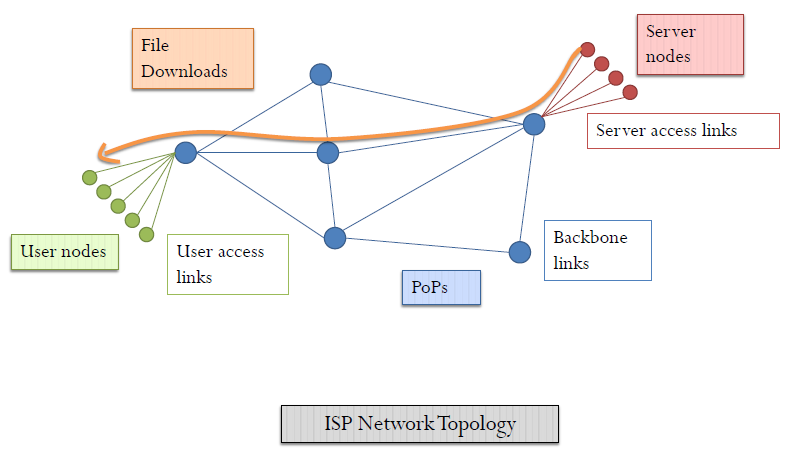
\includegraphics[scale=0.37]{final_images/expSetup.png}
% \end{center}
%\vspace{-0.1in}
%	  \caption{Diagram of an ISP network toplogy used in simulation}
%  \label{fig:isp_topology}
%\end{figure}


We translate a \textsl{TM} to a sequence of \textsl{File Arrivals} as follows. Suppose the traffic matrix entry from A to B is 100 Mbps and the duration being simulated is 200 seconds. During the experiment interval, we generate a sequences of file arrivals from A to B whose total size is 100Mbps $\times$ 200 seconds and the sizes are chosen from a realistic distribution.

A traffic engineering scheme \textsl{TE} calculates routing for \textsl{TM} based on a set of matrices \textsl{TM(-1)} which consists of either the current traffic matrix (for \opt) or a set of matrices from the previous traffic engineering {\em epoch} (for other TE schemes). The length of the epoch depends on {\em TE}, e.g., the epoch length for \optwt\  is 3 hours and for \cope\ is 1 day. When \textsl{TE}  yields a routing that splits flows across multiple paths between two nodes, the number of files assigned to each path is proportional to the flow along that path. We use  the source routing option in ns-2 to pin a file to a path. We note that the link utilization values obtained using this ns-2 methodology are consistent with those obtained using a simple linear program with the difference being at most 0.1.

%We are able to simulate matrices accurately using this method and the difference between empirical link utilization from ns-2 and the value obtained using a linear program based calculation is at most 0.1.

%We specify the path for each file using the source routing option in ns-2.


%\begin{table}[tb]\footnotesize
%    \subfigure[ISP Data]{\label{fig:ISP_data}
%  \begin{tabular}{ p{0.9cm} |  p{0.7cm} |  p{0.7cm} |   p{0.8cm} }
%\textbf{ISP} &\textbf{Nodes}  & \textbf{Links}  & \textbf{Duration of TM } \\ \hline
%US-ISP & 25 & 88 & 1hr\\ 
%Geant  & 22 & 68 & 15min \\
%Abilene & 12 & 30 & 5min	\\
%  \end{tabular}}
%    \subfigure[Bandwdith Distribution of Internet Users]{\label{fig:bandwidth_distribution}
%  \begin{tabular}{ p{0.7cm} | p{0.7cm} | p{0.8cm}  }
%\textbf{BW (Mbps)} &\textbf{US users \%}  & \textbf{Europe users \% } \\ \hline 
%0.25 & 4.9 &   1.5 \\
%2.0  & 38.1 & 26.2  \\
%5.0 & 32.4 & 57.8	\\
%10.0 & 20.0 & 14.5 \\
%20.0 & 4.6 & - \\
%  \end{tabular}}
%\caption{Simulation Data}
%\end{table}



In order to make the simulation complexity tractable, we scale down the topology and matrices.
ISP backbone link capacities run into tens of Gbps. Simulating such a network at scale even for 100 seconds would require sending data on the order of terabytes (or equivalently, a million 100KB files). Experimentally, we find that simulating at a tenth of this scale, i.e., 100K files, is feasible given the computational and memory constraints of our machines. A typical scale in our simulation is 1/20, i.e., we simulate the backbone link with 1/20 the capacity and also scale down the traffic between each source-destination pair accordingly.


%The scale of experiment determines the number of concurrent flows on a link. 

%A larger scale simulation has more concurrent flows in the network and makes the aggregate behavior more bursty.

\subsubsection{ISP topologies and traffic matrices}  We use datasets from the following three ISPs for our experiments:

\begin{figure*}\footnotesize
\begin{minipage}[b]{0.55\textwidth}
    \begin{tabular}{ l | c | c |   c }
%  \begin{tabular}{ p{0.9cm} |  p{0.7cm} |  p{0.7cm} |   p{1cm} }
\textbf{ISP} &\textbf{Nodes}  & \textbf{Links}  & \textbf{TM Duration} \\ \hline
Abilene & 12 & 30 & 5min	\\
&&&\\
Geant  & 22 & 68 & 15min \\
&&&\\
US-ISP & - & - & 1hr\\ 
  \end{tabular}
 \caption{ISP Data}
\label{fig:ISP_data}
\end{minipage}
\begin{minipage}[b]{0.45\textwidth}
  \begin{tabular}{ p{1.2cm} | p{1.5cm} | p{1.5cm}  }
\textbf{BW (Mbps)} &\textbf{US users \%}  & \textbf{Europe users \% } \\ \hline 
0.25 & 4.9 &   1.5 \\
2.0  & 38.1 & 26.2  \\
5.0 & 32.4 & 57.8	\\
10.0 & 20.0 & 14.5 \\
20.0 & 4.6 & - \\
  \end{tabular}
  \caption{Bandwidth Distribution}
\label{fig:bandwidth_distribution}
\end{minipage}
\end{figure*}

%
%\begin{figure}\footnotesize
%  \begin{center}
%    \begin{tabular}{ l | c | c |   c }
%%  \begin{tabular}{ p{0.9cm} |  p{0.7cm} |  p{0.7cm} |   p{1cm} }
%\textbf{ISP} &\textbf{Nodes}  & \textbf{Links}  & \textbf{TM Duration} \\ \hline
%Abilene & 12 & 30 & 5min	\\
%Geant  & 22 & 68 & 15min \\
%US-ISP & - & - & 1hr\\ 
%  \end{tabular}
% \caption{ISP Data}
%\label{fig:ISP_data}
%  \end{center}
%\end{figure}
%
%
%
%\begin{figure}\footnotesize
%  \begin{center}
%  \begin{tabular}{ p{1.2cm} | p{1.2cm} | p{0.8cm}  }
%\textbf{BW (Mbps)} &\textbf{US users \%}  & \textbf{Europe users \% } \\ \hline 
%0.25 & 4.9 &   1.5 \\
%2.0  & 38.1 & 26.2  \\
%5.0 & 32.4 & 57.8	\\
%10.0 & 20.0 & 14.5 \\
%20.0 & 4.6 & - \\
%  \end{tabular}
%  \end{center}
%  \caption{Bandwidth Distribution}
%\label{fig:bandwidth_distribution}
%\end{figure}
%


(1) \textbf{Abilene}, from the publicly available Abilene ISP data \cite{abilene}.
(2) \textbf{Geant}, the un-anonymized version of the Geant topology obtained from the TotemData \cite{TotemData} project personnel. 
(3) \textbf{US-ISP}, a large Tier-1 ISP topology obtained from authors of  \cite{MultiTM}.  TMs for all ISPs were logged in the period from 2004-2005. Figure \ref{fig:ISP_data} shows number of nodes, number of links, and the interval at which TMs are logged for each ISP.  The number of nodes and links for US-ISP is proprietary information.


%
%We used three datasets for our experiments as shown in Figure \ref{fig:ISP_data} and described below.
%
%\noindent\textbf{Abilene:} We used the publicly available Abilene ISP topology and traffic matrices \cite{AbileneData} logged once every 5 minutes.
%
%\noindent\textbf{Geant:} We used the Geant topology and TM data for the Geant network  provided by the Totem project \cite{TotemData}. We used the un-anonymized version of topology obtained from the project personnel. The matrices are logged once every 15 minutes. 
%
%\noindent\textbf{US-ISP:} We used the anonymized PoP level topology and traffic matrices from a US Tier-1 ISP (labeled as US-ISP throughout the paper) logged once every hour over from Feb13-Feb26, 2005. We obtained this data from the authors of \cite{MultiTM}.

%
%\begin{enumerate}
%\item \emph{Abilene}: We used the publicly available Abilene ISP topology and traffic matrices \cite{AbileneData} logged once every 5 minutes.
%\item  \emph{Geant}: We used the Geant topology and TM data for the Geant network  provided by the Totem project \cite{TotemData}. We used the un-anonymized version of topology obtained from the project personnel. The matrices are logged once every 15 minutes.
%\item  \emph{US-ISP}: We used the anonymized PoP level topology and traffic matrices from a US Tier-1 ISP (labeled as US-ISP throughout the paper) logged once every hour over from Feb13-Feb26, 2005. We obtained this data from the authors of \cite{MultiTM}. 
%\end{enumerate}
%
%\begin{figure}
%\begin{center}
%  \begin{tabular*}{0.35\textwidth}{@{\extracolsep{\fill}}| c | c | c |  c |}
%    \hline
%\textbf{ISP} &\textbf{\# Nodes}  & \textbf{\# Links}  & \textbf{TM Interval} \\ \hline \hline
%US-ISP & 25 & 88 & 1hr\\ \hline
%Geant  & 22 & 68 & 15min \\ \hline
%Abilene & 12 & 30 & 5min	\\ \hline
%  \end{tabular*}
%\caption{ ISP Data }
%\label{fig:ISP_data}
%\end{center}
%\end{figure}

\subsubsection{Simulation parameters}
Unless otherwise stated, we choose the following parameters for all of our simulations. Our goal is to choose parameters that are close to realistic values for ISPs.
% further discussion about the sensitivity of our results to the choice of these parameters is in Section~\ref{sec:discuss}.

\noindent\textbf{Scale:}  We experiment with Abilene, Geant and US-ISP datasets at  scales 1/10, 1/20 and 1/100 respectively. These are the largest scales we can experiment with for each network given our computational constraints.

\noindent\textbf{Duration:}  The simulation duration for most experiments is 300 seconds. We verified that running the simulations for longer durations did not qualitatively affect our results. Note that the duration here refers to the real time being simulated in ns-2, not the system time required to run the simulation.


\noindent\textbf{Bandwidth of users:} We use the bandwidth distribution of Internet users from the  ``State of the Internet Report'' \cite{Akamai-soti} released by Akamai, one of the largest commercial content distribution networks in operation today. Figure \ref{fig:bandwidth_distribution} tabulates this data for US and Europe.

\noindent\textbf{File sizes:} We simulate three file sizes of 100KB, 1MB and 10MB respectively contributing to  8\%, 3\% and 89\% of the total traffic respectively. These values are the fractions of traffic due to small files ($<$200KB), medium size files (200KB to 2MB), and large files ($>$2MB) in the Internet. We obtained these numbers by collating data from multiple sources \cite{urlinternet,kazaa,youtubestudy,pareto}.

%Typically, the average size of web files is less than 10KB, but we used a smallest file size of 100KB to limit the number of files in the simulation. The download rate of 100KB files using TCP is more sensitive to RTT since they may complete download even in slow start phase.
%Since we measure download rate of files, 10MB files would have similar file download rates as larger files

\noindent\textbf{Link delay:} We calculate the propagation delay of backbone links from geographic distances between nodes for Geant and US-ISP. For Abilene, we measure the propagation delay of backbone links using \emph{traceroute} and \emph{ping} between PlanetLab \cite{Planetlab} nodes in cities where the PoPs are located. All links use drop-tail queuing.

%\noindent\textbf{Queuing:} We have used Drop Tail queuing at all links.

\noindent\textbf{File inter-arrival time:} We  assume an exponential distribution of file inter-arrival times.


%\noindent\textbf{Router Buffer Size:} We set the router buffer sizes at the access and backbone links to the average bandwidth-delay product \cite{routerbuffersize} which is still widely used in production networks \cite{ExpRouterBuffer}. We defer further investigation of the impact of smaller router buffer sizes  \cite{routerbuffersize} to future work.  
% on the interaction between TE schemes and application performance

%\noindent\textbf{Link queue capacity:} We set the router buffer sizes at the access and backbone links to the average bandwidth-delay product \cite{routerbuffersize}. We note that although proposals for significantly smaller buffer sizes have been experimentally verified for backbone links networks \cite{ExpRouterBuffer}, this rule of thumb is still widely reflected in routers deployed in production networks \cite{ExpRouterBuffer}. We defer further investigation of the impact of smaller buffer sizes on the interaction between TE schemes and application performance to future work.

\subsubsection{Computational resources}
We use a shared cluster of 60 machines. Each machine has a 8-Core Intel Xeon processor and 16GB of memory. Each ns-2 simulation consists of 300--500s of simulated time and 10K to 200K file downloads, which results in a memory footprint of up to 10GB and takes between 1 to 48 hours to complete.

\subsection{Traffic engineering schemes} We select a subset of TE schemes reflecting a variety of proposed approaches in the literature including optimal TE (\opt), demand-oblivious TE (\invcap) and demand-aware TE (\optwt, \mplsavg\ and \cope).

{\bf{\opt}}, the minimum MLU TE scheme for a TM. We consider it as being representative of {\em online} TE schemes.

%a TE scheme that minimizes the maximum link utilization (MLU) for a given traffic matrix. We consider it as being representative of online TE schemes.

{\bf{\invcap}}, a simple routing scheme that does not ``engineer'' traffic, but instead  simply relies on shortest-path routing using the inverse of the link capacity as the link weight. \invcap\ is a common default routing protocol supported by popular commercial router vendors \cite{InvCapCite}.

{\bf{\optwt}},  a shortest-path routing algorithm using link weights computed using a heuristic algorithm to optimize a cost function \cite{fortz2000internet}. We use its implementation in the Totem Toolbox \cite{TotemData}. Typically, ISPs recompute routes a few times a day based on a set of measured TMs, so we simulate \optwt\ by computing a new routing every 3 hours based on the average of matrices in the past 3 hours.

%a TE scheme widely used by ISPs\cite{FortzThorup2} that engineers link weights for a given traffic matrix (TM) such that shortest-path routing using those weights for that matrix minimizes a specific cost function. Typically, ISPs recompute routing a few times a day based on a set of measured TMs, so we simulate \optwt\ by computing a new routing every 3 hours based on the average of matrices in the past 3 hours.  We use the implementation of the Fortz-Thorup algorithm available in the TOTEM toolbox \cite{TotemData} to compute the optimal link weights for a TM. This algorithm minimizes a convex cost function based on link utilization described in \cite{FortzThorup} and used in several follow-on papers.

{\bf{\mplsavg}}, a TE scheme that minimizes the MLU in an {\em offline} manner. Similar to \optwt, \mplsavg\ recomputes a new routing once every 3 hours based on average of TMs in past 3 hours.

%Unlike \opt\ above that uses the most recent matrix to recompute routing frequently (on the order of minutes), \mplsavg\  computes a routing so as to minimize the MLU for a matrix averaged over the past 3 hours TMs.

{\bf{\cope}}, a TE scheme that minimizes the common-case MLU while limiting the worst-case MLU caused by unpredictable spikes in the traffic matrix. We use the authors' implementation and parameters settings, and recompute routes once a day based on the previous day's TMs  as in \cite{COPE}.


{\bf{\mindelay}} scheme minimizes average latency for all traffic, unlike the schemes above which optimize link utilization based metrics.
Specifically, the objective function \mindelay\ optimizes is $\sum_{e \in E} d_e T_e$, where $E$  is the set of all links, $d_e$ is the propagation delay of link $e \in E$, and $T_e$ is the total traffic (in bits/sec) for $e\in E$. 
We evaluate \mindelay\ to answer whether user-perceived performance improves if we optimize latency instead of MLU.
We constrain the linear program so that MLU does not exceed 0.6, thereby ensuring that high link utilization does not hurt user-perceived  performance.
Like \opt, \mindelay\ has perfect knowledge of traffic matrix.


%\noindent{\bf{\cope}}, a TE scheme that seeks to minimize the MLU while limiting the worst-case link utilization caused by unpredictable spikes in the traffic matrix. As described in the paper \cite{COPE1}, COPE recomputes routing once a day so as to minimize the MLU for a matrix that is averaged over matrices observed during the previous day while limiting the worst-case link utilization resulting from any matrix lying within the convex hull of matrices observed during the previous day. We obtained the code for COPE from the authors and used their parameter settings throughout our experiments.
  
% COPE's optimization formulation optimizes measured traffic matrices and limits worst case link utilization during unpredictable spikes in traffic. We compute a new routing once every day as in the paper\cite{COPE1}. The performance ratio parameter is set to 2.2. We use the authors' code for experiments. 







\begin{figure*}[tbh]
  \begin{center}
%    \subfigure[Mean download rate]{\label{fig:allisps_mean_throughputs}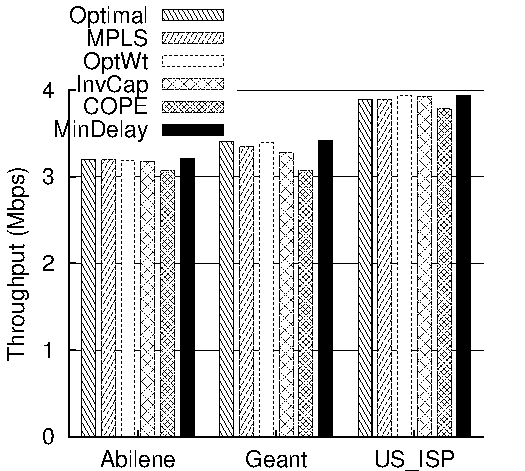
\includegraphics[width=35mm,height=30mm]{final_images/mean_throughput_hist_plot.pdf}}
    \subfigure{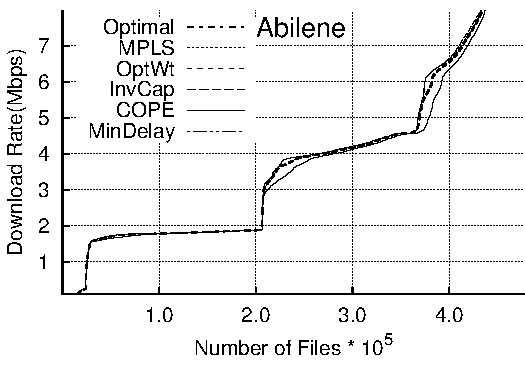
\includegraphics[scale=0.55]{final_images/G3_CDF/Abilene_download_rates_aggregate_plot.pdf}}
    \subfigure{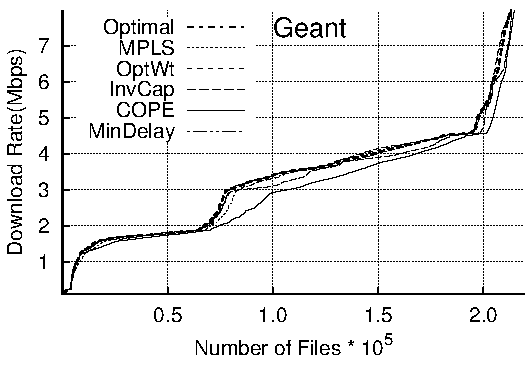
\includegraphics[scale=0.55]{final_images/G3_CDF/Geant_download_rates_aggregate_plot.pdf}}
    \subfigure{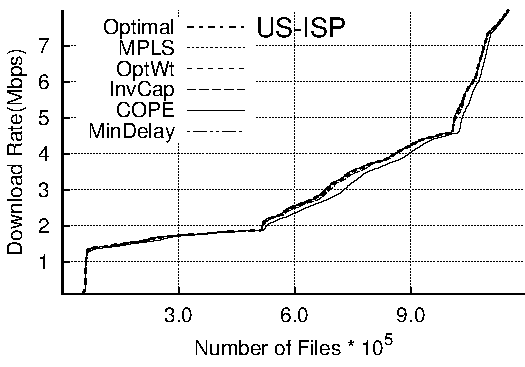
\includegraphics[scale=0.55]{final_images/G3_CDF/ATT_download_rates_aggregate_plot.pdf}}

  \end{center} 
  \caption{Download rate CDFs for all TE schemes are near identical except \cope\ which has slightly lower performance}
  \label{fig:throughputs_CDF}
\end{figure*}

\section{User-perceived performance}
\label{sec:app_performance}
In this section, we present a comparative analysis of the impact of different TE schemes on user-perceived performance. A summary of our findings is as follows. First, all TE schemes  including \invcap\ show nearly identical user-perceived performance for TCP and UDP traffic. Second, different TE schemes do achieve different MLUs as expected, suggesting that MLU is a poor predictor of user-perceived performance. Third, COPE consistently performs slightly worse than all other schemes in TCP throughput, suggesting that accounting for unpredictable variations in traffic hurts the common case user-perceived performance.

%we present our comparison of traffic engineering schemes based on simulation of traffic matrices at Internet loads for 3 ISPs. Our simulation shows that unexpectedly that all traffic engineering schemes (even \invcap) perform near identical in terms of download rates using TCP for all ISPs. We also show that MLU a metric commonly used metric for traffic engineering does not predict TCP throughput well and traffic engineering which optimizes for unexpected traffic variations increases delay and hurts TCP throughput.

%In this section, we present our comparison of traffic engineering schemes based on simulation of traffic matrices at Internet loads for 3 ISPs. Our simulation shows that unexpectedly that all traffic engineering schemes (even \invcap) perform near identical in terms of download rates using TCP for all ISPs. We also show that MLU a metric commonly used metric for traffic engineering does not predict TCP throughput well and traffic engineering which optimizes for unexpected traffic variations increases delay and hurts TCP throughput.

%Prior works on traffic engineering have measured its performance using linear programming simulation and have used metrics such as the maximum link utilization or similar cost functions based on link utilization.


\subsection{TCP performance}

We simulate TMs from 2 days of data for each ISP. For each day, we simulated 50 matrices measured at 5-minute intervals for Abilene, 25 matrices measured at 15-minute intervals for Geant, and 24 matrices measured hourly for US-ISP. We present results for the second day. The metric of user-perceived performance is the \emph{download rate} of files using TCP, where the file arrival workload is generated using the traffic matrices as described in Section \ref{sec:sim_TM}.

%\begin{figure}
%\begin{center}
%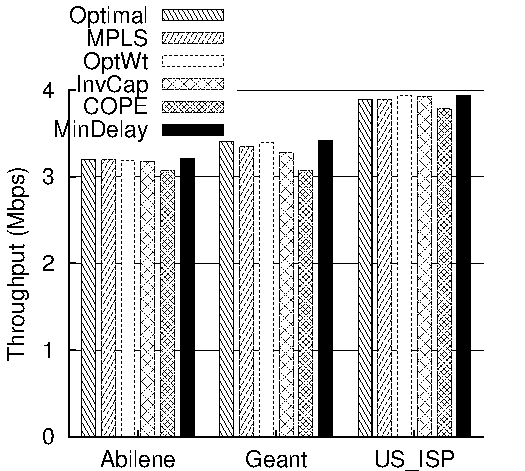
\includegraphics[scale=0.6]{final_images/mean_throughput_hist_plot.pdf}
%\caption{Mean download rates}
%\end{center}
%\label{fig:allisps_mean_throughputs}
%\end{figure}
%
%\begin{figure}
% \begin{center}
%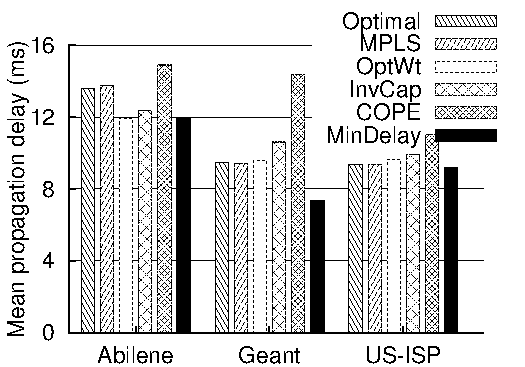
\includegraphics[scale=0.6]{final_images/G4_propdelay/mean_prop_delay_plot.pdf}
%\caption{COPE has the highest propagation delay among TE schemes}
% \end{center}
% \label{fig:prop_delay_all}
% \end{figure}


Figure \ref{fig:allisps_mean_throughputs} shows the mean download rate of files, where the average is across all files across all of the simulated matrices for each TE scheme.
We make three observations from this graph. 
First, all schemes achieve nearly same mean download rates with the exception of COPE that is consistently worse by up to  10\%.
Next, \opt\ (the leftmost bar in each group) is not always the best as minimizing MLU is not the same as optimizing TCP performance.
Finally,  \mindelay\ (the leftmost bar in each group) that optimizes latency performs the same as other TE schemes that optimize link utilization based metrics.


Figure \ref{fig:throughputs_CDF} shows the corresponding CDFs for the mean download rates in Figure \ref{fig:allisps_mean_throughputs}. The CDFs show that the near-identical TCP performance achieved by all TE schemes is not an artifact of presenting a specific statistic such as the mean, but is reflected by the entire distribution.  All distributions show a stepwise increase which suggests that access links are a bottleneck for a significant fraction of file transfers. This observation partly explains why \mindelay\ fails to  improve TCP throughput over other schemes: TCP throughput cannot be improved for flows bottlenecked at access link even if \mindelay\ scheme reduced the RTT for these flows.

\begin{figure*}[t]
\begin{minipage}{0.45\textwidth}
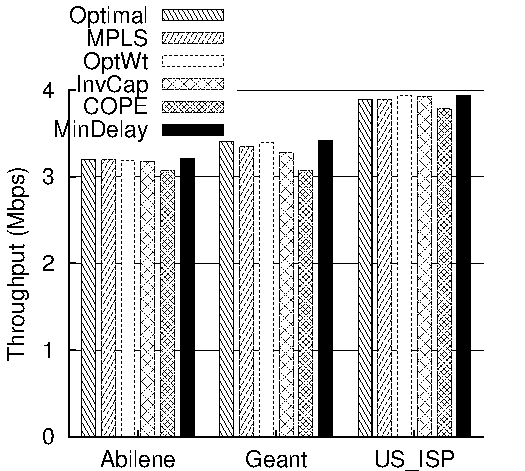
\includegraphics[scale=0.6]{final_images/mean_throughput_hist_plot.pdf}
\caption{Mean download rates}
\label{fig:allisps_mean_throughputs}
\end{minipage}
\hspace{1cm}
\begin{minipage}{0.45\textwidth}
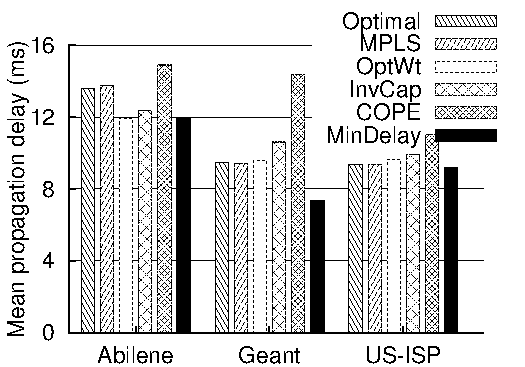
\includegraphics[scale=0.6]{final_images/G4_propdelay/mean_prop_delay_plot.pdf}
\caption{COPE has the highest propagation delay among TE schemes}
 \label{fig:prop_delay_all}
\end{minipage}
\end{figure*}

% we present the download rate of all files from all traffic matrices during the day sorted in increasing order  and in Figure ~\ref{fig:allisps_mean_throughputs} we show the mean value of the above distribution.

%What is result ?
%The download rate curves for all traffic engineering schemes are strikingly similar for all the topologies. Even the simple routing scheme, \invcap{}  has mean and median throughputs within 5\% of \opt{}  for all 3 topologies.  \opt{} does not have any additional gain over other routing schemes in download rate. The only notable difference is throughput is for \cope{} which has up to 10\% lower median throughput than \opt{} for Geant toplogy and has lowest throughput among all schemes. All 3 graphs show a step-wise increase which shows that access link are bottleneck for a significant fraction of file transfers.


%
%\begin{figure}[htb]
%  \begin{center}
%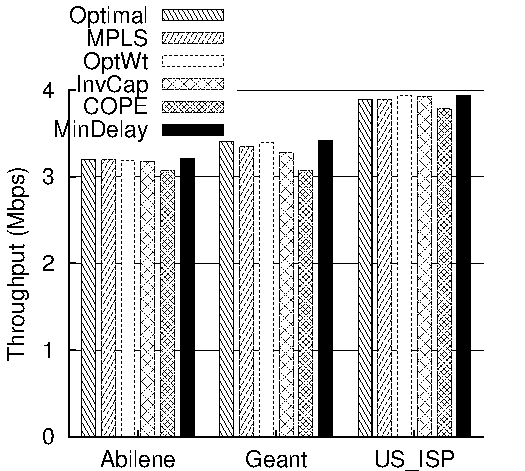
\includegraphics[scale=0.5]{final_images/mean_throughput_hist_plot.pdf}
% \end{center}
%	  \caption{Mean download rates of files for Internet traffic matrices}
%  \label{fig:allisps_mean_throughputs}
%\end{figure}




%\begin{figure*}[tbh]
%  \begin{center}
%%    \subfigure[Mean download rate]{\label{fig:allisps_mean_throughputs}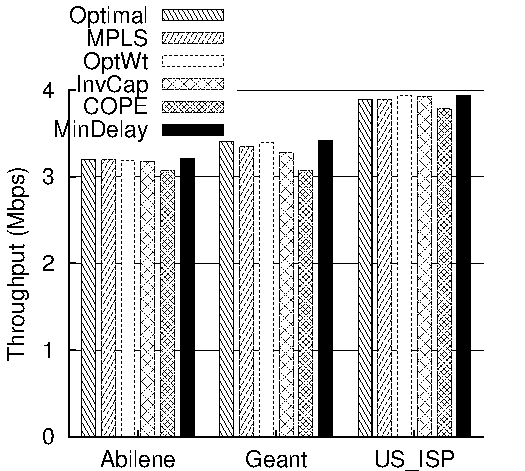
\includegraphics[width=35mm,height=30mm]{final_images/mean_throughput_hist_plot.pdf}}
%    \subfigure[Download rate CDF Abilene]{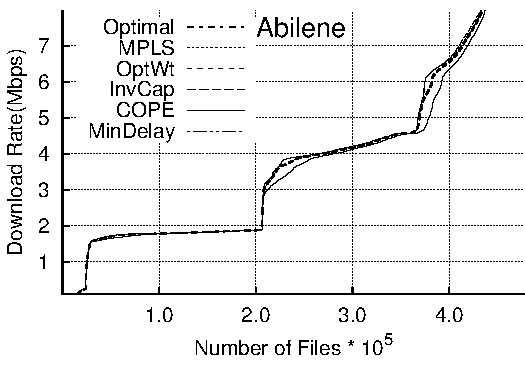
\includegraphics[scale=0.6]{final_images/G3_CDF/Abilene_download_rates_aggregate_plot.pdf}}
%    \subfigure[Download rate CDF Geant]{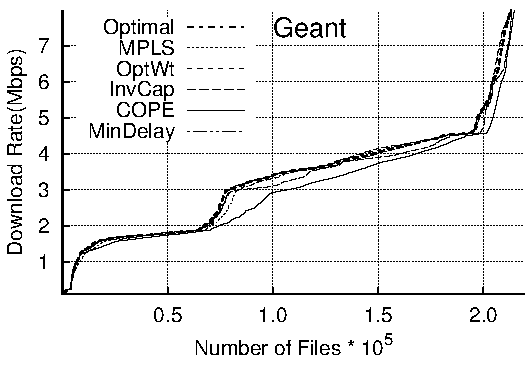
\includegraphics[scale=0.6]{final_images/G3_CDF/Geant_download_rates_aggregate_plot.pdf}}
%    \subfigure[Download rate CDF US-ISP]{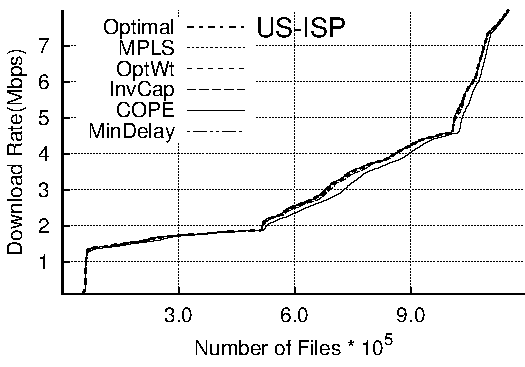
\includegraphics[scale=0.6]{final_images/G3_CDF/ATT_download_rates_aggregate_plot.pdf}}
%  \caption{Download rate CDFs for all TE schmes are near identical except \cope\ which has slightly lower performance}
%  \label{fig:throughputs_CDF}
%  \end{center} 
%\vspace{-0.2in}
%\end{figure*}

%\subsection{Analysis}
%Here, we present an analysis of above results using additional statistics measured from simulation.

\subsubsection{MLU vs. TCP performance}

To further investigate the results in Figure \ref{fig:allisps_mean_throughputs} and Figure \ref{fig:throughputs_CDF}, we analyze the empirically observed MLU for all TE schemes in the experiments. Figure \ref{fig:All_ISPs_MLU} plots the MLUs for all matrices considered. For US-ISP the MLU data is proprietary, so we present the ratio of MLU with respect to \opt. As expected, different TE schemes do show substantially different MLUs. For example, the MLU for \invcap\ and \optwt\ is up to twice the MLU of \opt\ in some cases; \mindelay\ has a MLU of 0.6 on Geant, which is more than twice of \opt's MLU. These results suggest that MLU is a poor predictor of download rate performance: schemes with near-identical TCP throughput have very different MLUs, and COPE despite achieving near-optimal MLU consistently shows sub-optimal TCP throughput.

%\textbf{MLU:}
%The above results may seem surprising if we observe the empirical MLU of all the traffic matrices simulated (Figure ~\ref{fig:All_ISPs_MLU}). The graphs show a significant difference among traffic engineering schemes. MLU for \invcap{} or \optwt{} is up to twice the MLU of \opt{} in many cases. The contrast between MLU and download rate graphs leads us to the conclusion that a higher MLU for Internet traffic matrices does not imply a worse TCP performance. We observe that \cope{} has a MLU close to \opt{} in Geant and US-ISP topologies but its download rate is lower than all other TE schemes. This is because \cope{} has greater path delay. This shows that even a low MLU traffic engineering scheme can have a worse TCP performance.

The main reason why MLU does not affect download rate is because queuing delay and loss rates are negligible until link utilization reaches a threshold. In our experiments, link utilization below 0.7 causes near negligible loss rates and queuing delays. Since the MLUs on most of the traffic matrices are below this value, loss rates on backbone links minimally impact the throughput of file downloads.  These observations are consistent with a recent  study on Level-3 ISP network  \cite{ExpRouterBuffer} showing that loss rates on backbone links are zero even at 95\%  link utilization. This threshold is expected to be higher for actual backbone traffic as our experiments are at scale 1/10 or smaller. At larger scales, there would be more concurrent flows resulting in less bursty traffic and lower loss rates.

%The main reason why MLU does not affect download rate is because queuing delay and loss rates are negligible until link utilization reaches a threshold. We observe this in our simulation and this phenomenon has also been observed for backbone traffic in the Internet \cite{ExpRouterBuffer}. Since the MLUs on most of the traffic matrices are below this threshold, loss rates on backbone links minimally impact the throughput of file downloads.  These observations are consistent with a recent study on Level-3 network\cite{ExpRouterBuffer} showing that loss rates on backbone links are zero even at 95\%  link utilization. In our simulations, the threshold at which links exhibit non-negligible loss is around 0.7. This threshold is expected to be higher for actual backbone traffic as our experiments are at scale 1/10 or smaller. At larger scales, there would be more concurrent flows resulting in less bursty traffic and lower loss rates.


The second reason why MLU hardly impacts the average download rate as well as the distribution is because it is largely determined by the traffic of only one link. Even under high MLU, the rest of the network may not be congested. File download rates are affected only for flows on this link, which may be a tiny fraction of the total traffic.




%There may exist intermittent traffic congestion which cause higher loss rates on backbone links. These happen due to interdomain routing changes \cite{BGPloss} (which are frequent) or due to anomalous traffic spikes in the Internet. An intradomain TE protocol cannot gurard against losses due to interdomain routing changes. It can be argued that doing \opt{} TE (using online traffic engineering) or a  TE scheme similar to \cope{} which is robust to traffic fluctuations would perform better in case of traffic spikes. These two routing schemes do not show any gain compared to other offline traffic engineering schemes in our experiment.  We infer that either these spikes are short enough to affect the average traffic matrices measured in our data set or the ISP networks are well provisioned to handle the spikes.


%\begin{figure}[tbh]
%  \begin{center}
%\includegraphics[scale=0.6]{final_images/G4_propdelay/i_o_diff_plot.pdf}
%  \end{center}
%  \caption{Propagation delay for Internet TMs.}
%  \label{fig:prop_delay_all}
%\end{figure}



\begin{figure*}[tb]

  \begin{center}
\subfigure{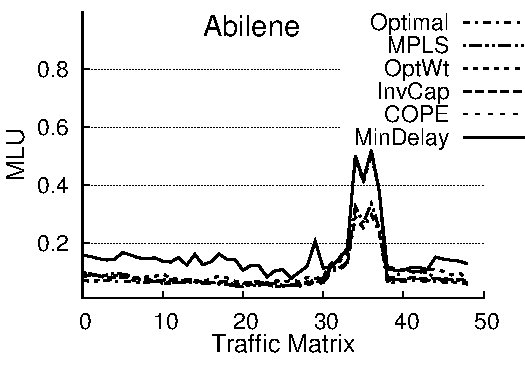
\includegraphics[scale=0.55]{final_images/G2_MLU//Abilene_MLUAverageUtilTable_plot.pdf}}
\subfigure{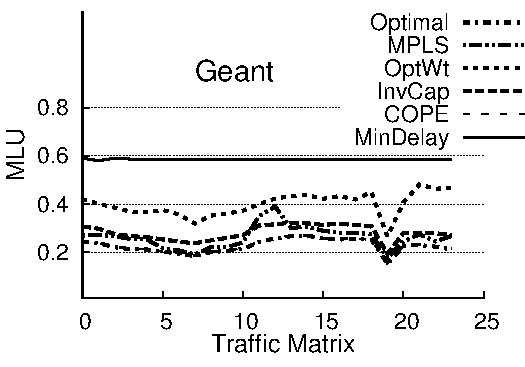
\includegraphics[scale=0.55]{final_images/G2_MLU//Geant_MLUAverageUtilTable_plot.pdf}}
\subfigure{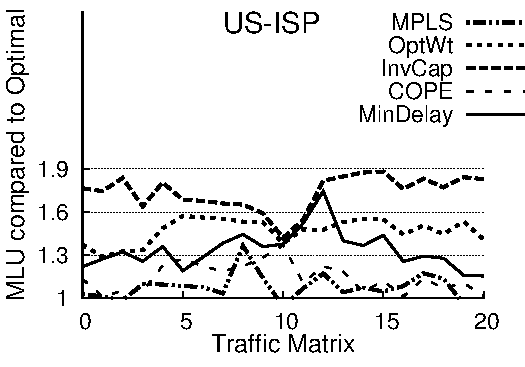
\includegraphics[scale=0.55]{final_images/G2_MLU//ATT_MLUAverageUtilTable_plot.pdf}}
  \end{center}
  \caption{TE schemes differ as much as 2$\times$ in MLU}
  \label{fig:All_ISPs_MLU}
  \end{figure*}
  
  
 
%\begin{minipage}{1.9in}
%  \begin{center}
%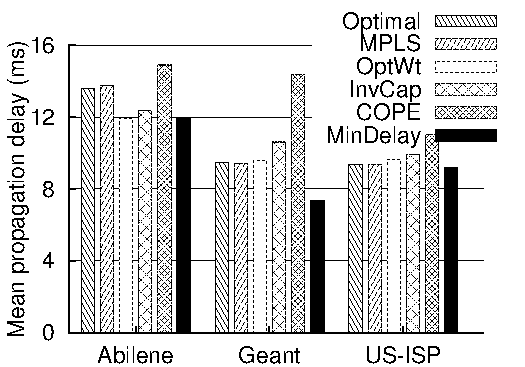
\includegraphics[scale=0.6]{final_images/G4_propdelay/mean_prop_delay_plot.pdf}
%  \end{center}
%  \caption{}
%
%
%  \label{}
%\end{minipage}
%\vspace{-0.2in}


\subsubsection{The price of predictability}
Why is \cope's performance consistently worse than the other schemes? To investigate this, we analyzed the propagation delays of routes computed by COPE. Given uniformly low loss rates and queueing delays, propagation delays primarily determine TCP performance.

Figure \ref{fig:prop_delay_all} shows the path delay averaged across all files and across all matrices for the different TE schemes. \cope{} has a significantly higher delay compared to all other schemes. We attribute this phenomenon to \cope{}'s optimization approach, which engineers for unpredictable spikes in traffic demands. Specifically, \cope\ attempts to bound the worst-case MLU for any traffic matrix similar to oblivious routing like schemes \cite{Cohen}. \cope\ intentionally routes some traffic along longer paths so as to leave room for occasional traffic spikes along shorter paths. While this approach makes \cope\ robust with respect to MLU under rare spikes in traffic, it comes at the cost of hurting common-case user-perceived performance.  Although we have not experimented with other oblivious routing schemes, these results suggest that any oblivious routing scheme that attempts to optimize MLU, e.g., \cite{Cohen}, is likely to incur a similar penalty in  user-perceived performance in the common case. 

%Although prior work has recognized that TE schemes can increase path delay, e.g.. \cite{TeXCP06}, to the best of our knowledge, our work is the first to empirically quantify the impact on TCP throughput and to show that engineering for rare traffic spikes comes at the cost of hurting common-case TCP throughput.

%It is known that TE schemes can increase path delay \cite{TeXCP06}. Our contributions are to show that \cope\ has a significantly higher path delay than other TE schemes and  to accurately measure the impact of increased path delay on TCP throughput. 


%This statistic explains why \cope{} has the lowest download rate among all schemes for Geant and US-ISP topologies. Our finding also suggests that other oblivious routing schemes which optimize for MLU \cite{ObliviousRouting} may have lower TCP throughput.

%We infer that the robustness of \cope to unpredictable traffic spikes comes at the cost of higher path delay and reduced TCP througput.  


%We observe that in Geant and US-ISP topologies \cope has lower mean and median value than other schemes. It is because the routing computed by \cope has a higher path delay compared to other traffic engineering schemes. We show the average propagation delay for all TE schemes in ~\ref{fig:prop_delay_all}. This statistic is the average of propagation delay of each file in our simulation. Different routings have same file request sequence but their paths depend on the routing. All TE schemes except \cope have similar path delay. The higher delay is significant for Geant and US-ISP topologies which explains its lower throughput. 

%\textbf{Users' Access Link Capacity:}

%Access link capacity is the  bottleneck for majority of file downloads in Figure ~\ref{fig:throughputs_CDF} but this may not hold true in Internet. The reasons are that paths have more delay (e.g. intercontinenal links), the access link at the server may be a bottleneck. Both these observations  affect all TE schemes identically and are unlikely to affect our findings. 

%It may be argued that our findings would not hold if Internet users had higher access link capacities. To verify this hypothesis, we also performed experiments where users access links had twice the current access link capacities. Our results remained unchanged  \cite{TechReport}.


%The minimum value of download rate in Figure ~\ref{fig:throughputs_CDF} is near zero in our simulation. This is because of congestion at the access link of users. In some cases a new file download starts on the same user node before previous download has finished. The previous flow has a large window size and sends many more packets than the new flow. In some cases, this causes multiple packet losses	 at access link queue for the new flow. Repeated timeouts due to these loss result in near zero download rates for some files. 

% Summary of result
%In this section we presented our comparison of traffic engineering schemes for file download rates in Internet. Our novel simulation based comparison has following main results: (1) All traffic engineering schemes (even \invcap{}) performs near identical in file download rate for Internet traffic matrices. (2) MLU is a poor predictor of TCP throughput : \invcap{} which has 2x higher MLU than \opt has nearly the same throughput and \cope{}'s MLU is near optimal but its throughput is lowest. (3) A traffic engineering approach such as \cope{} which engineers for unpredictable traffic demands increases path delay and reduces TCP throughput.

\subsection{UDP performance}
\label{sec:UDP_perf}
\subsubsection{Measuring UDP performance}

We assume that the loss rate and the queuing delay on each link for UDP traffic is the same as that measured during experiments with TCP traffic. This assumption is reasonable as TCP accounts for over 90\% of Internet traffic \cite{SprintBackbone}. We calculate the loss rate and delay for a path by combining the loss rates of links along the path; we compute the delay by summing the propagation and queuing delay of links along the path.

We compare performance of VoIP traffic (which uses UDP) using Mean Opinion Score (MOS). MOS is an industry standard VoIP call quality metric for which a score of above 4 is considered good and below 3 is considered bad. We calculate MOS using the formula in \cite{MOS-formula}  which calculates MOS given the loss rate and delay for a path. 

We calculate MOS for VoIP calls between all pairs of source and destination PoP nodes in an ISP. First, we measure loss rates and queuing delay on backbone links for each 10-second interval.  For each interval, we calculate the MOS for a path based on its end-to-end loss rate and delay. The mean MOS for a path is the average value of MOS over all intervals. For TE schemes that split traffic across multiple paths between a source-destination pair, the mean MOS for a source-destination node pair is calculated as the weighted average of mean MOS weighted by the fraction of the traffic split along each path between the node pair. We similarly calculate the 5th percentile MOS for a source-destination pair by taking the weighted average of 5th percentile MOS values for all its paths.

\subsubsection{Results}
We obtain a distribution of mean MOS values for a TE scheme by combining mean MOS values for all pairs of source and destination nodes for all traffic matrices. We find that the minimum and the maximum values of mean MOS for all TE schemes are in the range (4.08, 4.14) for Abilene, (4.07, 4.14) for Geant and (4.08, 4.14) for US-ISP.  The range of values for 5th percentile MOS are (4.07, 4.13) for Abilene, (4.08, 4.14) for Geant and (4.05, 4.14) for US-ISP. MOS scores for all schemes are always above 4.0 and the differences between different TE schemes is at most 0.1. These results are not surprising since loss rates and queuing delay are near-negligible for most links in the network. Furthermore, MOS is not very sensitive to few milliseconds difference in propagation delay among TE schemes.




%\tbd{In summary, our study of the impact of state-of-the-art TE schemes on application performance reveals the following. All TE schemes have near-identical TCP throughput and UDP performance for a VoIP call quality metric. }

	


%The only exception is \cope\ that has a slightly lower TCP throughput, which is because it attempts to absorb unpredictable variations in traffic at the cost of common case application performance. Furthermore, we find that the commonly used MLU metric is a poor predictor of TCP performance. Taken together, these results suggest that the simplest routing scheme, \invcap, suffices to achieve similar performance as sophisticated traffic engineering schemes proposed in the literature or in use in production networks today.

%Our experiments in this section showed that all traffic engineering schemes perform near identical in terms of TCP throughput for traffic matrices from 3 ISPs in the Internet. Even though traffic engineering schemes differ by as much as twice in terms of MLU, their TCP throughput is identical because of near zero loss rates and queuing delay on most links. An interesting observation is that \cope which has MLU close to \opt has a lower TCP throughput.

%In the following section, we experiment with traffic matrices at higher load than current Internet and study the effect of application adaptation.


%In FIgure ~\ref{fig:All_ISPs_MLU} we show the maximum link utlization for the traffic matrices we experiment with. The graphs show a significant difference among traffic engineering schemes. MLU for \invcap or \optwt being upto twice the MLU of \opt but these differences are not reflected in throughputs. Higher link utliizations cause increased loss rates and higher queuing delay for packets. We find that in our experiments both these values remain near-zero until link utilization values of 0.6 in our experiments. Since the MLU on most of the traffic matrices are below this threshold value, MLU isnt a factor in the throughput of file downloads. Even if the utilization on one link is high enough to increase loss rates on that link the rest of the network may not be facing any congestion. File downloads rates are affected only for flows on this link, which could a small fraction of total traffic.


%In Fig ~\ref{fig:allisps_aggregate_InternetBW}, we also show the CDF of TCP throughput for all files for US-ISP topology . This shows that access link is the bottleneck for a large fraction of file transfers in our simulation. This helps us explain the near identical values for all routings. This observation is likely to be different for internet since paths have more delay (e.g. intercontinenal links ), the access link at the server may be a bottleneck, and there may exist intermittent traffic congestion which cause higher loss rates on backbone links. The first two reasons affect all TE schemes identically and are unlikely to affect our findings. The third reason intermittent congestion on backbone in internet can happen beacuse of interdomain routing changes [cite sprint study] ( which are frequent ) or due to anomalous traffic spikes in the internet. An intra domain TE protocol cannot gurard against losses due to interdomain routing changes. It can be argued that doing \opt TE ( using online traffic engineering ) or a  TE scheme similar to \cope which is robust to traffic fluctuations would perform better in case of traffic spikes. Since these two routing schemes do not show an improvement compared to other offline traffic engineering schemes, either these spikes are short enough to affect the average traffic matrix over 15 min or 1 hour period or the spikes do not cause performance degradation for internet traffic matrices for all TE schemes.


%It must be noted that our experiments are at scale 1:10 to 1:50. At, higher scale the loss rate and queuing delay would be lower at the same link utilization level. As scale increases, the router buffer sizes increase and the per packet processing time decrease proportionally. If we take the analogy from a queuing model such as $M/M/1/K$ queue, at higher loads the mean packet arrival rate ($\lambda$), the mean packet processing rate($\mu$) and the capacity of the queue ($K$) increase proportionately. The formula for loss rates of this queuing model show that both these metrics decrase as $\lambda$, $\mu$  and $K$ increase proportioately \cite{queue}. If anything , the scale of our experiments reinforces our results that MLU has minimal application performance in realistic ISP topologies. 


%\subsubsection{Comparison of path delay}
%
%In Fig ~\ref{fig:prop_delay_all}, we present the average propagation delay for TE methods. The propagation delays presented are the average propagation delay for all file transfers.  The notable outlier in the table is \cope which has the highest delay in all three topologies. It delay is maximum in Geant where it has 25\% higher delay than the next highest delay TE method. This explains the the reason for \cope having lower throughput than other TE schemes. All other TE methods have delay within 1ms of each other for Abilene and US-ISP. Their near identical througputs reflect this trend.
%
%We calculate this statistic from the traffic matrix and routing computed by a TE method. First, we calculate the delay of tranfers between a source destination pair by multiplying the propagation delay by the total traffic on each path. The sum of this delay for all source destination pairs gives the total delay for a traffic matrix. The total propagation delay is the sum of delays of all trafic matrices divided by the sum of all traffic matrices.


%
%\begin{figure}
%\begin{center}
%  \begin{tabular}{| l | c | c | c | }
%    \hline
%Routing & Abilene & Geant & US-ISP \\ \hline \hline
%\opt &  4.54 &	9.46 & 9.37\\ \hline
%\invcap & 4.13 &10.62 & 9.90 \\ \hline
%\mplsavg & 4.58 & 9.40 & 9.37\\ \hline
%\cope &4.97 & 14.38 & 11.03\\ \hline
%\optwt & 3.98 & 9.57 & 9.64\\ \hline
%MinDelay & 3.97 & 7.34 & 9.21\\ \hline
%  \end{tabular}
%\caption{Propagation delay (in ms) for TE methods on different topologies}
%\end{center}
%\label{fig:prop_delay_all}
%\end{figure}

%\subsection{Effect of access link bottlenecks}
%
%We measure the effect of access link capcity of users on our results by experimenting at higher capacity access link bottlenecks. A reasonable choice for higher access link bottleneck is doubling current the access link capacities. In Table ~\ref{fig:all_isps_internetBWx2} shows the mean throughputs for all 3 ISPs. The mean throghputs increase by 1.3-1.7 times but the relative difference between different routings remain the same. This shows that throughputs of different traffic engineering schmes are near identical because of current traffic load in the network and would remain identical even if the current internet bandwidths were much higher.
%
%\begin{figure}[tbh]
%  \begin{center}
%\includegraphics[scale=0.7]{newImages/mean_throughput_twice_internetBW.jpg}
%  \end{center}
%  \caption{Mean throughputs of file transfers at twice internet access link bandwidths}
%  \label{fig:all_isps_internetBWx2}
%\end{figure}

%\begin{figure}
%\begin{center}
%  \begin{tabular}{| l | c | c | c | }
%\hline
%Routing & Abilene & Geant & US-ISP \\ \hline \hline			
%\opt	&	589.5	&	720.6	&	671.1	\\ \hline
%\\invcap	&	580.6	&	721.9	&	640.1	\\ \hline
%\mplsavg	&	589.4	&	720.0	&	654.1	\\ \hline
%\cope	&	560.4	&	695.4	&	587.8	\\ \hline
%\optwt	&	586.2	&	723.1	&	662.2	\\ \hline
%MinDelay	&	589.8	&	723.9	&	663.9	\\ \hline
%  \end{tabular}
%\caption{Mean throughputs at twice the internet access link bottlenecks}
%\end{center}
%\label{fig:all_isps_internetBWx2}
%\end{figure}

%\begin{figure*}[htb]
%  \begin{center}
%    \subfigure[Download rate US-ISP]{\label{fig:edge-a}\includegraphics[scale=0.4]{newImages/US_ISP/internetBW_scale2/download_rates_aggregate_plot.pdf}} 
%    \subfigure[Download rate Geant ISP]{\label{fig:edge-a}\includegraphics[scale=0.4]{newImages/Geant/internetBW_scale2/download_rates_aggregate_plot.pdf}} 
%    \subfigure[Download rate Abilene ISP]{\label{fig:edge-a}\includegraphics[scale=0.4]{newImages/Abilene/internetBW_scale2/download_rates_aggregate_plot.pdf}}  
%    \subfigure[Download ratio US-ISP]{\label{fig:edge-b}\includegraphics[scale=0.4]{newImages/US_ISP/internetBW_scale2/opt_download_ratios_aggregate_plot.pdf}} 
%    \subfigure[Download ratio Geant ISP]{\label{fig:edge-b}\includegraphics[scale=0.4]{newImages/Geant/internetBW_scale2/opt_download_ratios_aggregate_plot.pdf}} 
%    \subfigure[Download ratio Abilene ISP]{\label{fig:edge-b}\includegraphics[scale=0.4]{newImages/Abilene/internetBW_scale2/opt_download_ratios_aggregate_plot.pdf}} 
%  \caption{US Tier 1 ISP, Aggregate performance on 1 day traffic matrices,twice today's internet access link bottleneck distribution }
%  \end{center}
%  \label{fig:allisps_aggregate_internetBWX2}
%\end{figure*}

%As an interesting aside, we present the results for no access link bottlenecks in Fig  ~\ref{fig:allisps_aggregate_nolimit} .
%
%\begin{figure*}[htb]
%  \begin{center}
%\subfigure[US-ISP]{\label{fig:edge-c}\includegraphics[scale=0.75]{newImages/ATT_nolimit_Download_ratio_aggregate_plot.pdf}}
%\subfigure[Geant]{\label{fig:edge-c}\includegraphics[scale=0.75]{newImages/Geant_nolimit_Download_ratio_aggregate_plot.pdf}}
%\subfigure[Abilene]{\label{fig:edge-c}\includegraphics[scale=0.75]{newImages/Abilene_nolimit_Download_ratio_aggregate_plot.pdf}}
%  \end{center}
%  \caption{All ISPs : Download ratios for 1 day traffic matrices, without access link bottlenecks}
%  \label{fig:allisps_aggregate_nolimit}
%\end{figure*}

%\subsection{Experiments at higher scale}
%As said previously in this section, our simulations at lower scale provide a more challenging environment for comparison. To experimentally validate our findings at a higher scale, we selected 5 traffic matrices from each ISP and repeated our simulation at a higher scale. We simulated Abilene and Geant topology at original scale and the US-ISP topology at scale 1:10. We present the aggregate download ratios for 5 traffic matrices for at scale 1:50 and scale 1:10. The download ratios curve highlight the difference between traffic engineering schmes more clearly. The shape of the curves look almost the same in both graphs. This shows that our results remain consistent even at higher scale.
%
%Thus our results for 3 ISPs based on ns-2 simulations show that under traffic conditions in the internet the throughput performance of all traffic engineering schemes differ are near identical. Our results are consistent even at higher acess link botttlenecks in the internet and on experiment at higher scale. These findings show that difference in MLU for TE schemes does not translate to an improvement in throughput in internet conditions. Propagation delay is a more important factor and traffic engineering schemes which increase propagation delay have lower throughputs. 

%
%\subsection{Application Performance at higher loads}
%
%\subsubsection{Single Download Location}
%
%\subsubsection{Multiple Download Downloads}

\section{Capacity and location diversity}
\label{sec:capacity}
%things to do to ready  section 5

%A. Relative Input-Output Difference
%	- Rewrite example
%	- update y-axis \maxiodiff{} on graph, update caption 
%	- Write formal proof

%B. Simulating application adaptation ..
%	- improve writing

%C. Experimental procedure
%	- make changes suggested by Aditya

%D. Capacity increase with location diversity
%	
%	1. LP:

%	- finish writing
%	- update graphs
%	- check values
%	- update linear program in appendix
%	
%	2. ns-2 simulations:
%	
%	- update data based on simulations
%	- calculate confidence intervals
%	- replot graphs
%	- rewrite results

%E. Capacity increase with fraction of location diversity traffic
%	- get data in new format
%	- plot graph in gnuplot
%	- write subsection

%F. Write summary paragraph

%\textbf{intro to section}




%The results in the previous section show that different TE schemes yield nearly identical application performance at traffic demands encountered today. In this section, we compare TE schemes with respect to their potential capacity, i.e., the ability to accommodate surges in the traffic demand. In contrast to most prior work, our capacity analysis incorporates the ability of applications to leverage location diversity, i.e., the ability to download content from multiple locations. Our main findings are that (1) location diversity can significantly increase (by up to 2$\times$) the capacity achieved by all engineering schemes; (2) even a modest amount of location diversity (e.g., the ability to download content from two locations) enables all engineering schemes to achieve near-Optimal capacity; (3) with location diversity even simple routing scheme of \invcap\ has at most 30\% less capacity compared to \opt.

The results in the previous section may seem unsurprising---different TE schemes yield nearly identical user-perceived performance simply because today's low traffic demand levels obviate the need to engineer traffic. However, in this section, we show that similar conclusions hold when we compare TE schemes with respect to their potential capacity, i.e., their ability to accommodate surges in traffic demand in the future.

The key factor that explains our unexpected findings is location diversity, i.e., the ability to download content from multiple locations. Our main findings are that (1) location diversity can significantly increase the capacity (by up to 2$\times$) achieved by all engineering schemes; (2) even a modest amount of location diversity (e.g., the ability to download content from two locations) enables all engineering schemes to achieve near-Optimal capacity; (3) with location diversity even simple routing scheme of \invcap\ has at most 30\% less capacity compared to \opt.


%We next compare TE schemes based on their capacity for Internet traffic demands. Our focus is on application adaptation due to location diversity, an important trait of Internet traffic, that has largely been ignored in prior work.

%To this end, we first address two main challenges: (1)  How to design an experiment to simulate application adaptation ? (2) How to decide empirically whether the network is below or above capacity for a traffic demand ? Later, we present comparison results using two approaches :
%(1) Using a linear program to calculate the maximum capacity for a network with location diversity.
%(2) Using ns-2 to simulate application adaptation in the form of parallel downloads of files

%Our results verify our initial hypothesis that location diversity increases the capacity of a network. Surprisingly we find that it can significantly reduce capacity difference among TE schemes (except \invcap{}).


%\subsection{Quantifying capacity}

%\textbf{What is the metric ?}

%In general, the capacity achieved by a TE scheme can be quantified as a {\em region} that includes all of the traffic matrices that it can accommodate. However, quantifying the capacity of a TE scheme as a region may shed little light on its ability to tolerate typically encountered load spikes. Furthermore, it is cumbersome to compare TE schemes that achieve overlapping capacity regions. So, researchers commonly use a simpler metric such as the MLU to characterize the capacity with respect to a given traffic matrix. Intuitively, the inverse of the MLU serves as a metric of capacity, e.g., if a TE scheme achieves an MLU of 0.25 for a given matrix, then it can tolerate up to a 4$\times$ surge in the load represented by the matrix.

%For a traffic demand in the network, the relevant metric of capacity is how much surge in the traffic demand can the network tolerate. We denote  the surge in traffic demand by  \emph{load} of the traffic matrix. Our metric of comparison is \emph{the maximum load of the traffic matrix for which the network is below capacity}. We use the term SPF to refer to this metric. Clearly, a higher SPF value is better for a TE scheme.

%For a routing and a traffic matrix at a load $x$, we say that \emph{the network is below capacity for the traffic matrix at load $x$} if the traffic can be routed from source to destination nodes without exceeding the capacity on any link in the network.  This metric reflects how much surge in original traffic demand can the network sustain using a TE scheme. Henceforth, we refer to this metric as SPF.

%\textbf{ 1/MLU = CAP without adaptation}

%Prior work has compared TE performance using MLU.  MLU is related to SPF in some cases. If $\alpha$ is the MLU at load 1.0 for a traffic matrix, then SPF = 1/$\alpha$ assuming (1) traffic matrix entries increase linearly with load and (2) routing remains same at every load. In this case a lower MLU scheme can tolerate a greater surge in network traffic.

%
%\begin{figure}[htb]
%\begin{center}
%\subfigure[load = 1.0]{\label{fig:load-1}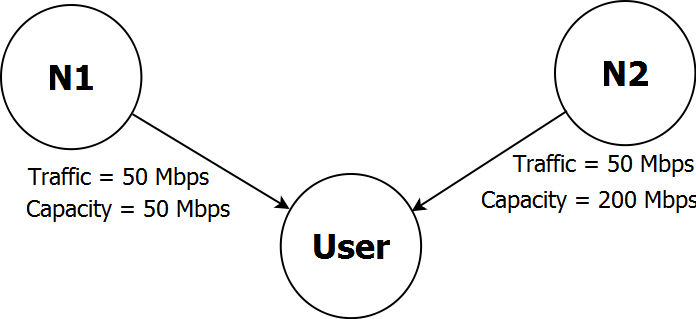
\includegraphics[scale=0.25]{final_images//Diagram1.png}}
%\subfigure[load = 2.0]{\label{fig:load-2}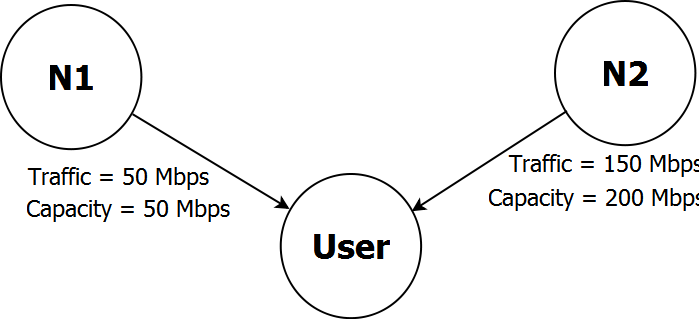
\includegraphics[scale=0.25]{final_images//Diagram2.png}}
%\subfigure[load = 3.0]{\label{fig:load-3}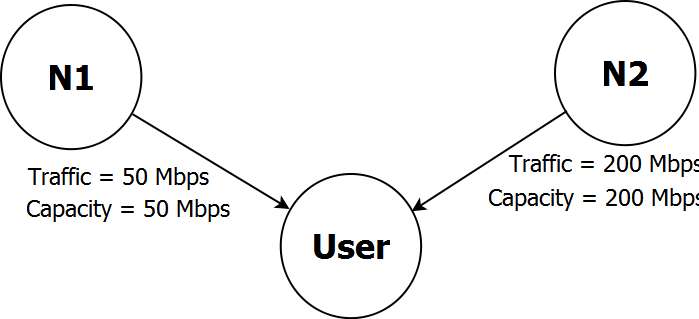
\includegraphics[scale=0.25]{final_images//Diagram3.png}}
%\end{center}
%\caption{Location diversity can change the traffic matrix}
%\label{fig:mlu_toy}
%\end{figure}
%

%\textbf{ but this does not hold with adaptation}

%Unfortunately, MLU is not a meaningful metric of capacity when application adaptation due to location diversity can change the traffic matrix itself. To appreciate this point, consider the example shown in Figure \ref{fig:mlu_toy}. Node 1 has a demand of 100 Mbps for content that can be fetched from either of nodes 2 or 3. Suppose node 1 splits the demand equally between the two locations, thereby resulting in an MLU of 1 by saturating the left link. Note that all TE schemes will result in the same routing as there is at most one route between each pair of nodes. Now suppose the demand at node 1 doubles to 200 Mbps. Node 1 can still satisfy its demand by fetching 50 Mbps and 150 Mbps along the left and right links respectively. Note that the MLU remains unchanged at 1 even though the demand has doubled. Furthermore, the doubling of demand does not simply scale the traffic matrix entries linearly, but instead changes them based on application behavior (e.g., based on how parallel TCP splits traffic across the two download locations). In general, it is difficult to predict how application behavior might change the traffic matrix as demand increases, as that change depends upon the underlying routing that in turn depends upon the original matrix. Indeed, even if the demand remains unchanged, the mere act of engineering routes (not observable in Figure \ref{fig:mlu_toy} as there is no route diversity) can change the traffic matrix when applications have location diversity.

%It is difficult to predict SPF using MLU if the network has application adaptation. This is because application adaptation can change the traffic matrix.  We show it using an example.  In Figure~\ref{fig:load-1} at load = 1.0 User node has a demand for 100Mbps traffic and it splits its demand equally and downloads 50Mbps each from N1 and N2. In Figure~\ref{fig:load-2}) at load = 2.0, the User node can still serve its demand by downloading 50Mbps from N1 and 150Mbps from N2. The metric MLU is not relevant in both cases since the application can change the traffic matrix to serve its demand. Empirically too we observed that the MLU value did not show a clear demarcation at a load where network is below capacity and the load where network is above capacity.

%\subsection{An empirical capacity measure}

%\textbf{proposing a new metric}

%We propose a new metric, {\em surge protection factor} (SPF), to quantify the capacity achieved by a TE scheme with respect to a traffic matrix. Let $E$ denote a TE scheme, $M$ the demand\tbd{Need to clarify that demand is a ``content matrix''.}, and MLU$(E,M)$ the MLU achieved by $E$ given $M$. When there is no location diversity, SPF$(E,M)$ is simply the inverse of MLU$(E,M)$, i.e., the factor of increase in the demand that can be satisfied. However, when there is location diversity, SPF$(E,M)$ is an {\em empirical} measure of the factor of increase in demand that can be satisfied, and is computed as follows. Let $kM$ denote the demand that scales each entry in $M$ by a factor $k>1$. Then, SPF$(E,M)$ is defined as the largest $k$ such that the routing computed by $E$ can satisfy the demand $kM$.

\subsection{Empirically measuring capacity}
Our metric of capacity is the SPF, i.e., the maximum surge in demand that can be satisfied (as  defined formally in Section \ref{sec:SPFdefinition}). Analytically determining whether an engineering scheme can satisfy a projected demand is difficult as it requires us to accurately model application adaptation  to location diversity, so the SPF must be determined empirically. In our experiments, we use a metric called {\em maximum input output difference} (or \maxiodiff) to determine whether a given demand can be satisfied. For each node, the {\em input} is the total traffic (bits/sec) requested by that node, while the {\em output} is the total traffic received by that node. \maxiodiff\ is defined as the maximum across all nodes of the relative difference between the input and output, i.e., {\em (input - output)/input}. If \maxiodiff\ is measured to be less than 0.1, then the demand is considered as satisfiable. We allow for a small difference in order to account for measurement error as well as to account for bursts in demand over the measurement duration.

%
%\begin{figure}
%\vspace{-0.1in}
%  \begin{center}
%\includegraphics[scale=0.55]{final_images/G5_IOdiff/i_o_diff_plot.pdf}
%  \end{center}
%  \caption{Profile of \maxiodiff{} at increasing surge factors for a Geant TM}
%  \label{fig:input_output_diff}
%\end{figure}
%
%  \begin{figure}
% \begin{center}
%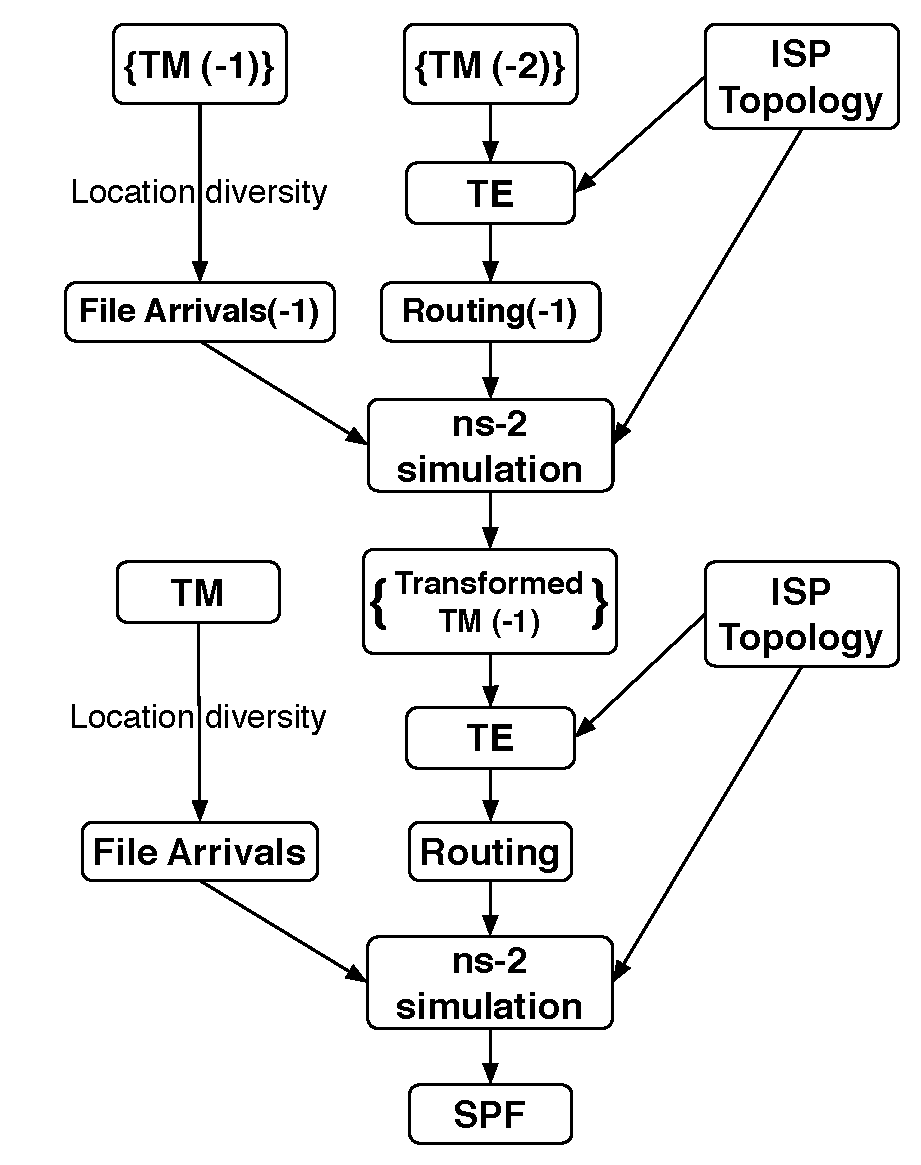
\includegraphics[scale=0.4]{final_images/Simulation2.pdf}
%\caption{Block diagram of experiment process with location diversity}
% \end{center}
% \label{fig:simulation2}
% \end{figure}


%\tbd{The reader may wonder why we could not have used the empirically measured MLU instead of \maxiodiff\ above, i.e., to consider a demand as satisfied if the measured MLU is less than 1 instead of of \maxiodiff\ is less than 0.1.}


% There are a couple reasons for this. First, the empirically measured MLU can never exceed 1, so the cutoff has to be a value somewhat less than 1. Second, as in the previous section, we find MLU to be a poor predictor of application performance, e.g., a higher MLU may result in equivalent or better application performance. This disparity between application performance and MLU only exacerbates under location diversity. We were unable to determine an empirical cutoff for the MLU that clearly delineates workloads that can be satisfied from those that can not.


%We propose a new metric to answer the above question - \emph{the maximum relative input-output difference}. Input for a node is the total traffic requested by users at the node. Output for a node is the total traffic received by users at the node. For each node with non-zero input, we compute its relative input-output difference as follows : Relative Input-Output Difference = (Input - Output)/Input. If input is zero for a node, we define its relative input-output difference as zero. Our metric is the maximum relative input-output difference over all nodes in the network. We will refer to this metric as \emph{\maxiodiff{}} from now on. 

%\textbf{use diagram to explain why it works}

%We illustrate this metric using the topology in Figure~\ref{fig:mlu_toy} again.  At load = 2.0 in Figure~\ref{fig:load-2} node User has demand for 200Mbps traffic. This demand is served by N1 sending 50Mbps and N2 150Mbps. In this case, the network has the capacity to serve demand and the \maxiodiff{} of the network is zero. At load = 3.0 in Figure~\ref{fig:load-3} traffic demand at User is 300Mbps and the total capacity of incoming links in 250Mbps. The network does not have capacity to serve this demand and the \maxiodiff{} is 50Mbps/300Mbps = 16.67\%. A positive value of \maxiodiff{} implies network does not have capacity for the demand.

%\textbf{more general than MLU}


%\textbf{Claim about metric}
%We make the following claim about this metric: 

%\emph{For a static traffic demand in the network, if \maxiodiff{} is p\%  (p $>$ 0), then network has capacity for p\% lesser traffic demand. It follows that if p = 0, network has capacity for the current demand.}

% If the network has capacity to serve the demand then p $=$ 0.
%We present a formal proof of the above claim in the Section~\ref{sec:appendix}.

%\textbf{How we measure it experimentally}

%We measure \maxiodiff{} in ns-2 simulations as follows: For each node, input is the sum of sizes of all files (measured in bytes) requested for download at the node. The output at the node is sum of the number of bytes of all files downloaded at the node. The difference is equal to the size of unfinished file downloads at the node. The relative input output difference for a node is the ratio of unfinished file downloads to the input and the \maxiodiff{} of the network is maximum relative input-output difference over all the nodes.

%\textbf{graph generated from simulation}


\maxiodiff\ helps clearly distinguish workloads that can be satisfied. For example, in Figure~\ref{fig:input_output_diff}, we show a \maxiodiff{} profile for five experiments at surge factors of 1, 2, 3, 4 and 5 for a Geant TM with \invcap{} routing.  The graph shows the \maxiodiff{} measured at intervals of 10 seconds throughout the simulation.
%The X-axis shows the progress of simulation. 
We ignore the first 50 seconds of simulation as the input significantly exceeds output at the start of simulation. We observe that beyond the initial period of fluctuation, \maxiodiff\ is relatively stable and below 0.1 for surge factors 1--3 that can be satisfied, but significantly higher for surge factors 4 and 5 that can not be satisfied.
%\tbd{Will it be helpful to show a graph for why MLU does not delineate the capacity point well?}.


\begin{figure*}
\begin{minipage}{0.45\textwidth}
\includegraphics[scale=0.55]{final_images/G5_IOdiff/i_o_diff_plot.pdf}
  \caption{Profile of \maxiodiff{} at increasing surge factors for a Geant TM}
  \label{fig:input_output_diff}
\end{minipage}
\hspace{1cm}
\begin{minipage}{0.45\textwidth}
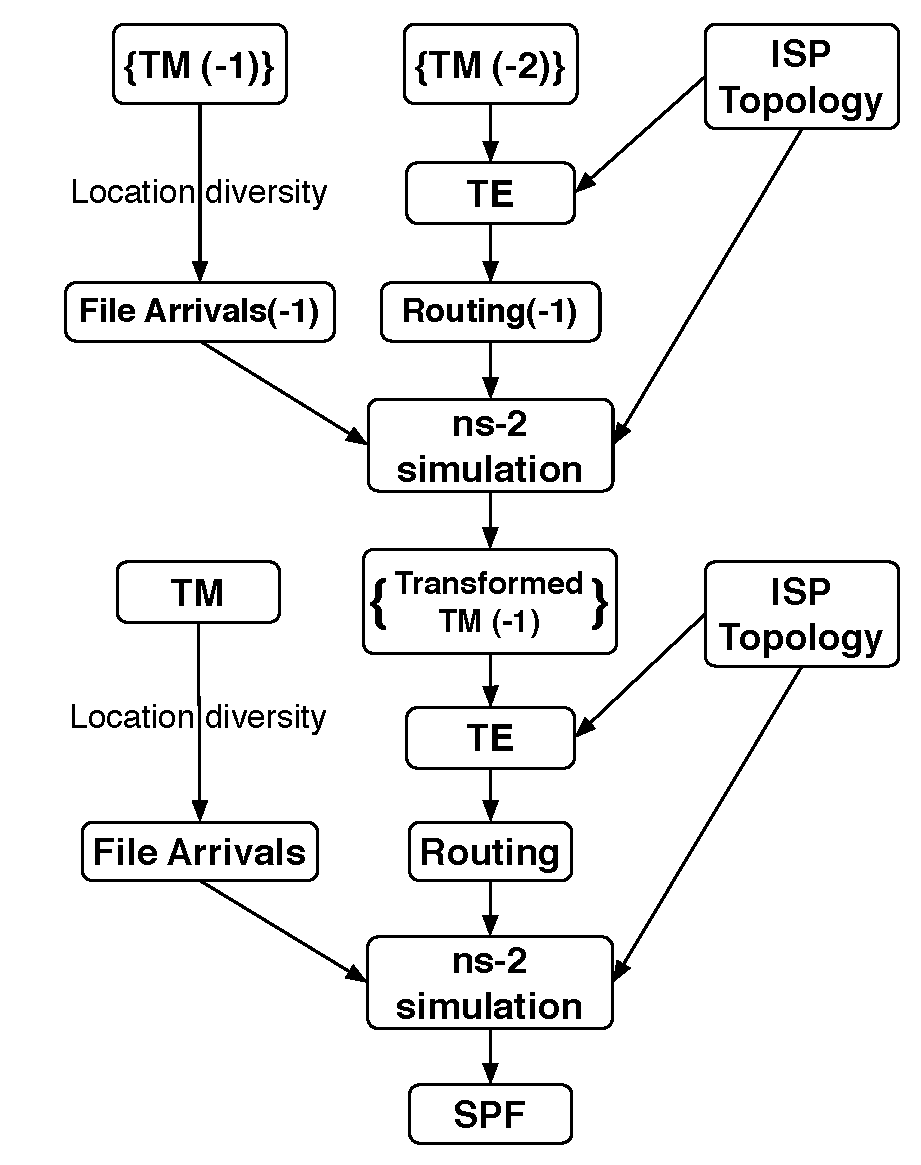
\includegraphics[scale=0.4]{final_images/Simulation2.pdf}
\caption{Block diagram of experiment process with location diversity}
 \label{fig:simulation2}
\end{minipage}
\end{figure*}


%Initial values vary significantly, but later the values vary within a range of a few percent and we infer that the \maxiodiff{} of the network lies in this range.

%
%\begin{figure}[t]
%  \begin{center}
%\includegraphics[scale=0.4]{final_images/G5_IOdiff/i_o_diff_plot.pdf}
%  \end{center}
%  \caption{Profile of \maxiodiff{} at increasing loads for a Geant TM and \invcap{} routing}
%  \label{fig:input_output_diff}
%\end{figure}

%\textbf{accommodating experimental errors}

%To decide if a network is has capacity for a given load, we need to accommodate two experimental artifacts: (1) As Figure~\ref{fig:input_output_diff} shows, the \maxiodiff{} varies within a few percent. Therefore, we take the average of 10 values of  \maxiodiff{} measured in the last 100s of simulation. (2) Experimentally, we observe that the  \maxiodiff{} is a small positive fraction even when the network has capacity. This is expected since we run our simulations for a short duration and some files have zero or very small download rates in our simulation. (This is explained in Section~\ref{sec:app_performance}). To account for it, we decide that the network has capacity at a given load if its \maxiodiff{} is less than 10\%. A 10\% error value in our simulation implies we can over predict the SPF of a network by at most 10\%. If we predict that the network has the capacity at load $x$ and $C$ is the SPF of the network, then $x < 1.1 C$.

%The average traffic demand for our simulation is static, therefore we can apply our claim stated above. According to our claim,  a 10\% difference in \maxiodiff{} implies that the network has is below capacity for a 10\% lesser demand.  

\subsection{Simulating location diversity}
\label{sec:ns2-multisource}

%An application can leverage location diversity in multiple ways. It can download in parallel from all locations or  download from the location which has the best performance (throughput/delay). Among these, we experiment with parallel downloads to model application adaptation. In our simulation, each file download is started simultaneously from all locations and file download finishes when total number of bytes downloaded from all locations equals the file size.

 
%\begin{figure}[tbh]
%  \begin{center}
%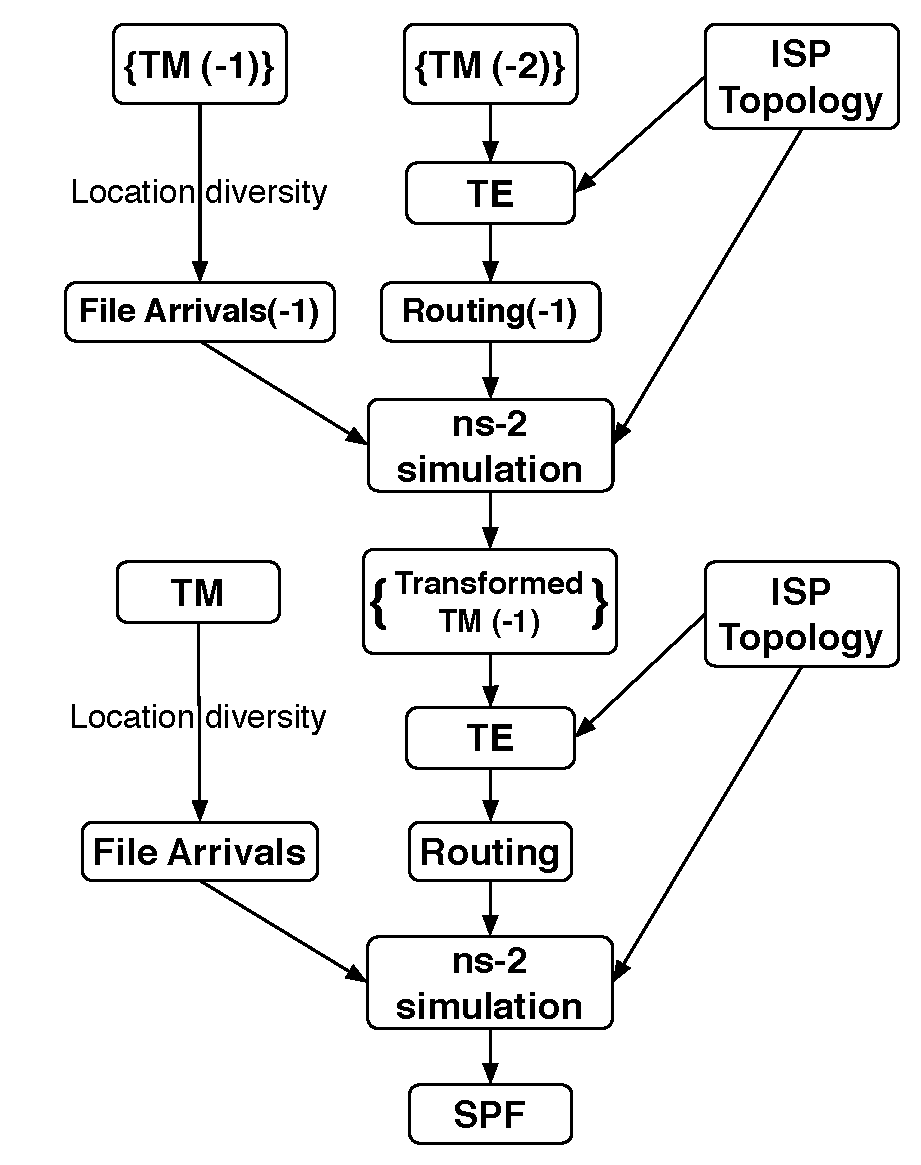
\includegraphics[scale=0.43]{final_images/Simulation2.pdf}
% \end{center}
%\vspace{-0.1in}
%	  \caption{Block diagram of experiment process with location diversity}
%  \label{fig:simulation2}
%\end{figure}

Figure~\ref{fig:simulation2} illustrates the experimental process with location diversity. The lower half  is similar to Figure~\ref{fig:simulation1} with two differences. First, to incorporate location diversity, we modify the procedure to transform {\em TM} to {\em File Arrivals} as follows. As in Section~\ref{sec:exp_setup}, we first transform PoP-to-PoP entries in {\em TM} to a sequence of file download requests. However, instead of downloading each file from just that one location, $k$-1  additional randomly chosen source locations are introduced so as to emulate a location diversity of $k$.  The file is downloaded in parallel from all $k$ locations using parallel TCPs. The download is considered complete when the total bytes downloaded across all $k$ locations equals the size of the file.

%except for the block \textsl{TM(-1)} that is replaced by \textsl{Transformed TM(-1)} in Figure~\ref{fig:simulation2}. The upper half of Figure~\ref{fig:simulation2} describes how \textsl{Transformed TM(-1)} is obtained from  \textsl{TM(-1)}.

%Another change which is not visible in the block diagram is the process of translating from \textsl{TM} to \textsl{File Arrivals}. This process is modified to incorporate the effect of location diversity. First we derive a sequence of  \textsl{File Arrivals} from  \textsl{TM} as described in Section~\ref{sec:exp_setup}. Then, we add ($k$ - 1) new locations, chosen randomly,  in addition to the original location from which each file can be downloaded.  $k$ is a location diversity parameter. Each file download initiates parallel TCP connections to the $k$ chosen locations in the network. A download is considered as completed when the total number of bytes download from all $k$ connections equals the size of the file.

Second, application adaptation to location diversity changes the input to {\em TE} as indicated by the block \textsl{Transformed TM(-1)} that is  obtained as follows. Let \textsl{TM(-1)} and \textsl{TM(-2)} respectively denote the (set of) matrix(ces) in the last and last-to-last epochs. Recall that {\em TE} determines the length of the epoch (0 for \opt, 3 hours for \optwt\ and \mplsavg\, and a day for \cope). \textsl{Transformed TM(-1)} is generated by the top simulation that takes as input the file arrivals obtained from \textsl{TM(-1)} and {\em Routing (-1)}. The latter is obtained by applying {\em TE} to \textsl{TM(-2)} in the previous epoch. This two-step simulation is intended to approximate the interaction of TE and application adaptation to location diversity that changes the TM. 

%the epoch length is determined by {\em TE} (e.g., \textsl{TM(-1)} is identical to {\em TM} for \opt\ but denotes the set of matrices in the most recent 3-hour ) The upper level simulation transforms 

%The need for \textsl{Transformed TM(-1)} arises because application adaptation to location diversity can change the traffic matrix.  \textsl{Transformed TM(-1)} is our estimate of the matrix resulting from the change in the matrix/matrices in the set \textsl{TM(-1)}. Note that \textsl{TM(-1)} is the either the current traffic matrix (for \opt) or the set of matrices from the previous  traffic engineering epoch (for other schemes). Using a ns-2 simulation, we simulate application adaptation for each matrix in \textsl{TM(-1)} and measure the resulting traffic matrix at the end of experiment.  The resulting set of matrices is \textsl{Transformed TM(-1)}.

%We do the simulation as follows (refer to Figure~\ref{fig:simulation2}): (1) Translate a matrix in \textsl{TM(-1)} to \textsl{File Arrivals} as described in the previous paragraph (2) Run \textsl{TE} algorithm to compute routing based on matrices in \textsl{TM(-2)}. Similar to \textsl{TM(-1)}, \textsl{TM(-2)} is either the current matrix (for \opt) or a set of matrices from the epoch \emph{before} the previous traffic engineering epoch (for other schemes). (3) Run \textsl{ns-2 simulation} using \textsl{File Arrivals}, \textsl{Routing} and \textsl{ISP Topology}. Finally, we measure the resulting traffic matrix.



%We start with a set of periodically logged traffic matrices from real ISPs in our dataset. Let $M_1, M_2,\cdots$ denote a sequence of such matrices and $E$ a TE scheme. As in the previous section, we translate each matrix $M_i$ to a file request arrival process. However, instead of downloading each file from just one location, we add $k-1$  randomly chosen source locations  from which the file is downloaded in parallel. The routes from the $k$ source locations to the sink are computed by applying $E$ to $M_i$. As a result of parallel downloads, each matrix $M_i$ will have changed, say, to a new matrix $N_i$.

%In the second step, we recompute routes by applying $E$ periodically to the appropriately time-averaged matrix. For example, if $E$ is \opt, we recompute routes periodically (once every 5, 15, or 60 minutes depending upon our ISP dataset) based on $N_i$ at that time instant. For \optwt, we recompute routes once every 3 hours using a matrix that is the average of the matrices in the past 3 hours, and so on. %We note that the recomputed routes and parallel downloads may again change $N_i$, resulting in a different MLU than engineered for, but this mismatch between engineering and application adaptation to location diversity is exactly what we seek to capture in our simulations.



%We note that an alternate form of location diversity is to download content from a single ``best'' location. However, we chose parallel downloads as they are simple, do not require any additional infrastructure for server selection, and are in widespread use in P2P systems today. 

%We define a location diversity parameter '$k$' - the number of locations content is present in the network.

%Experiments in this section include two types of ns-2 simulations : (1) Users download files from one source node only ($k = 1$) (2) Users download files in parallel from multiple locations ($k > 1$). We have already described our experiment with single location downloads. Our experiment with multiple locations is a two-step process which we explain next.





%We need two steps of simulation because application adaptation changes the traffic matrix. After the first step of simulation, we measure the adapted traffic matrix. In the next step, we compute routing based on the adapted traffic matrix.

%\subsubsection{Simulating a Traffic Matrix with Location Diversity}
%\textbf{why 1 ns-2 simulation is not accurate }
%Earlier while simulating single location download, we generated a file arrival sequence from the traffic matrix given. Next, we computed the routing based on current traffic matrix or a set of previous traffic matrices depending on routing. Then we simulated the arrival sequence in network with the given routing.

%A simple way to simulate a traffic matrix with location diversity is as follows: We compute the routing and we generate a file arrival sequence from the traffic matrix identical to single location download. But we choose (k - 1) additional source locations for each file. Then, we simulate parallel download of each file from k locations.

%But such a simulation does not ensure a fair comparison of TE schemes. The reason is that the traffic matrix resulting from parallel download simulation is likely to be very different from the original traffic matrix. But, the TE scheme had computed the routing assuming the original traffic matrix.

%Let S be the original set of TMs in our dataset and T $\in$ S be the TM we want to simulate with location diversity. The first step computes a file arrival process for this TM. The second step computes routing for this TM.

%\emph{First Step:} We compute a file arrival sequence for T identical to single location download. But we choose ($k - 1$) additional source locations for each file. Each file will be downloaded in parallel from these $k$ locations during the simulation. Since we split traffic among $k$ locations for each file download, it is expected that TM will be changed significantly during simultation.

%\emph{Second Step: } Computing a routing for T is difficult since we do not yet know the changed traffic matrix that will result from simulation. Routing for T may depend on T or a subset of other TMs in S as well. For example, \optwt{} computes routing on the average of past 3 hour TMs. These other TMs would also change due to location diversity which makes it more difficult to compute routing for T. We work around this problem as follows:  Through ns-2 simulations, we obtain a new set of TMs S' from set S which have changed due to location diversity in the network. We compute a routing for T based on the new set of TMs S'.

%We obtain the TMs in set S' as follows: For each TM in set S, we compute the routing and we generate a file arrival sequence from the traffic matrix identical to single location download. But we choose ($k - 1$) additional source locations for each file. Then, we simulate parallel download of each file from $k$ locations and measure the new traffic matrix. 


%\textbf{optimization}

%We optimize the simulation process by only computing those matrices in set S' which determine the routing for TM T. We compute the TMs depending on the TE scheme: \opt{} computes routing based on current TM, hence we only compute the adapted version of current TM; \optwt{} and  \mplsavg{} use the average of past 3 hour TMs, hence we average the TMs of past 3 hours from set S and compute its adapted version; \cope{} computes routing using all matrices from previous day but we use a random selection of 4TMs from previous day and compute routing using the adapted versions of these TMs;  the routing for \invcap{} is fixed.

\subsection{Experimental procedure}

%\textbf{experimental data and parameters}

The experiments to determine SPF involve a computationally intensive search across many different surge factors for each matrix. Furthermore, at high surge factors, the number of ns-2 data structures required to simulate ongoing parallel TCP connections becomes prohibitively high. So for computational tractability, we selected 4 matrices each from one day of data of each ISP. The matrices were selected randomly, one from each 6-hour duration during the day.  For each matrix and each engineering scheme, we conduct an experiment at each value of the surge factor starting from 1 in increments of 0.25 until the capacity point is reached, i.e., the \maxiodiff\ value exceeds 0.1. Each experiment is run until the \maxiodiff\ value stabilizes or 300 seconds, whichever is greater. 

%We selected only 4 TMs since we did 50-100 simulations with each TM. Experiments in this section were more computationally demanding since we experimented with higher loads which increased the number of file downloads we simulated and each file download used multiple TCP connections which increased the number of ns-2 data structures. Each experiment was run for 300s duration, but in some cases we did 500s experiments if the \maxiodiff{} didn't reached a stable value in 300s. Similar to Figure~\ref{fig:input_output_diff}, we compute \maxiodiff{} every 10 seconds.

%\textbf{how we calculate capacity}

%We calculated the SPF value by simulating a traffic matrix at increasing loads. We started with original TM (load 1), increased load by 0.25 at every step and checked if the network has capacity at that load. We select the highest load at which network had capacity as the SPF value.

%\textbf{upper and lower bounds}

%Our experimental procedure gives us following upper and lower bounds on the actual capacity of the network. If $x$ is the capacity we 
%measure and $C$ is the actual capacity, then : (1) $C < x + 0.25$. This is because we experiment with loads at intervals of 0.25. (2) We have already shown that $x < 1.1C $. Combining the upper and lower bounds for our experimental error \[x/1.1 < C < x + 0.25\]

%We use this equation to calculate confidence intervals for our results.

%% graphs for capacity using linear program
%\begin{figure}[t] \begin{center} 
%\subfigure[Abilene Optimal]{\label{fig:edge-a}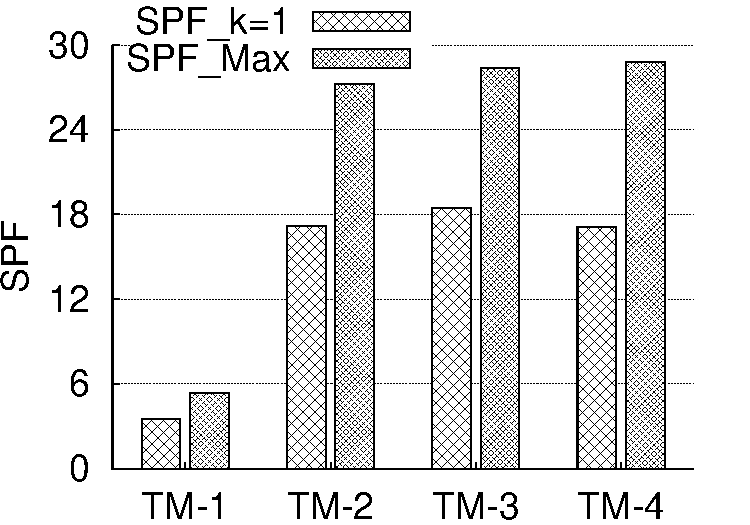
\includegraphics[scale=0.33]{final_images/G9_optcapacity/Abilene_opt_hist_plot.pdf}}
%\subfigure[Abilene InvCap]{\label{fig:edge-a}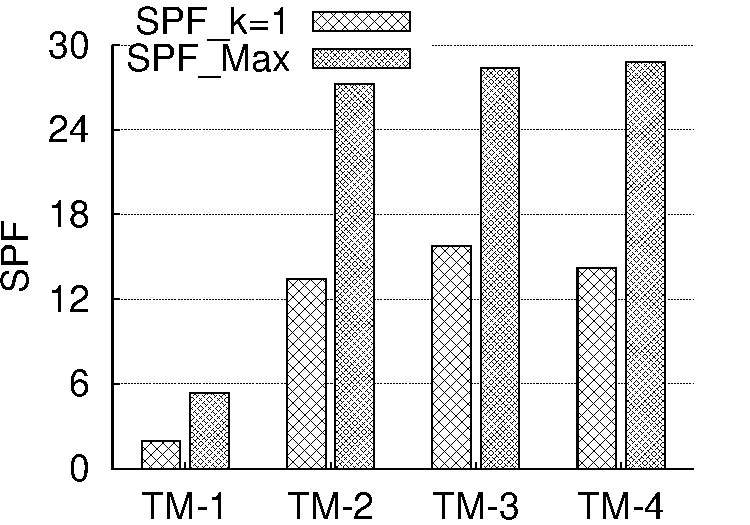
\includegraphics[scale=0.33]{final_images/G9_optcapacity/Abilene_inv_hist_plot.pdf}}
% \subfigure[Geant Optimal]{\label{fig:edge-b}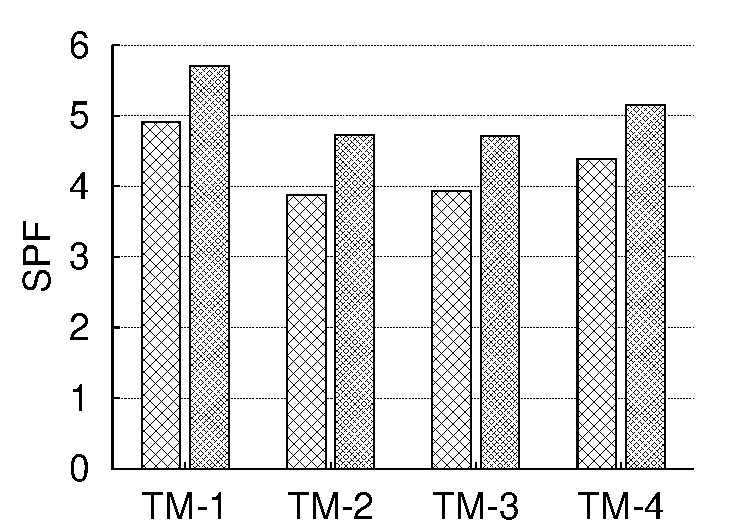
\includegraphics[scale=0.33]{final_images/G9_optcapacity/Geant_opt_hist_plot.pdf}}
% \subfigure[Geant InvCap]{\label{fig:edge-b}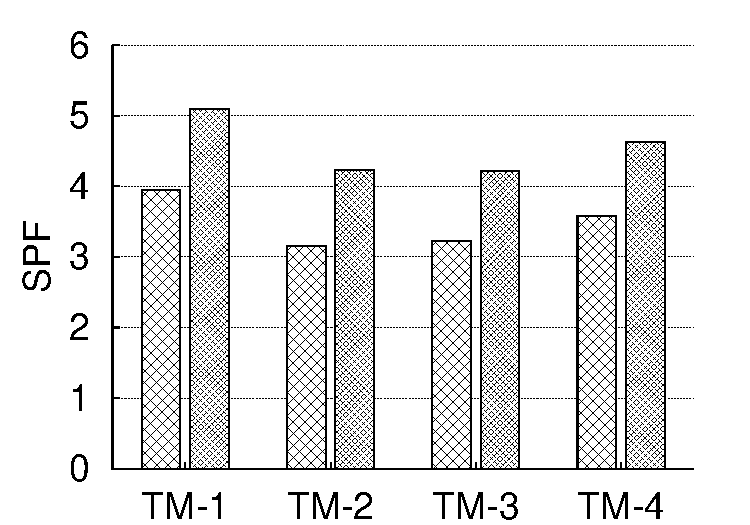
\includegraphics[scale=0.33]{final_images/G9_optcapacity/Geant_inv__hist_plot.pdf}}
%\subfigure[US-ISP Optimal]{\label{fig:edge-c}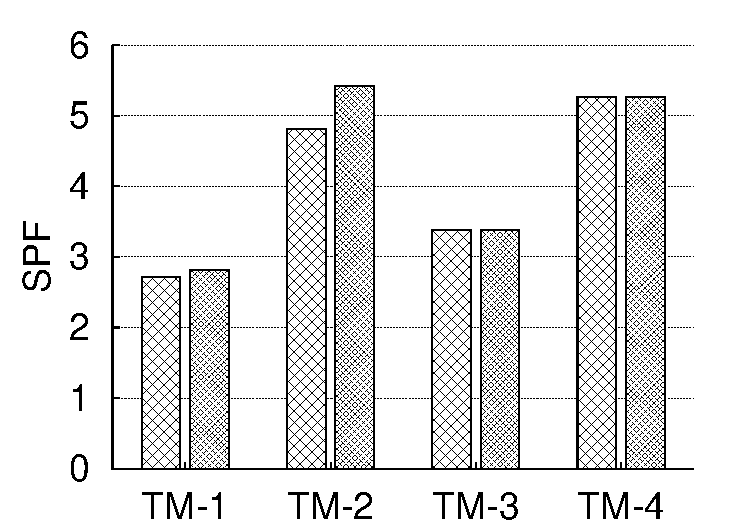
\includegraphics[scale=0.33]{final_images/G9_optcapacity/USISP_opt_hist_plot.pdf}}  
%\subfigure[US-ISP InvCap]{\label{fig:edge-c}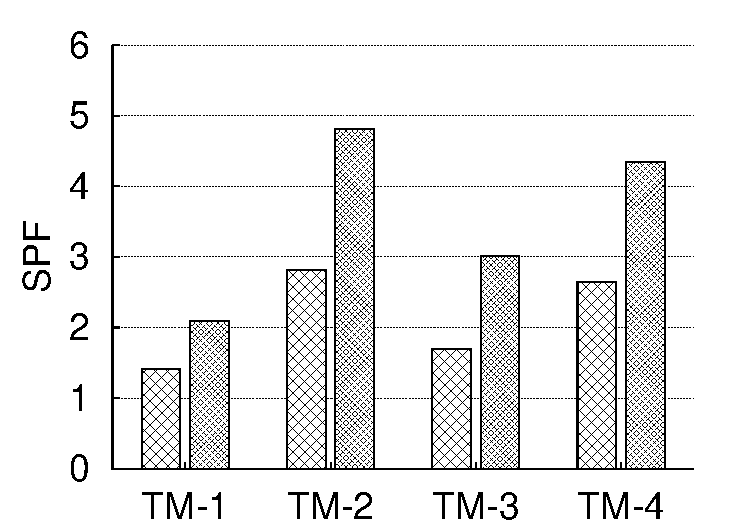
\includegraphics[scale=0.33]{final_images/G9_optcapacity/USISP_inv_hist_plot.pdf}}  
%\end{center}\caption{\label{fig:capacity_opt} Maximum SPF for \opt{} and \invcap{} routing calculated using linear program.}
%\vspace{-0.2in}
%\end{figure}


% graphs for capacity using ns-2 simulations


\begin{figure*}[t] \begin{center} 
\subfigure{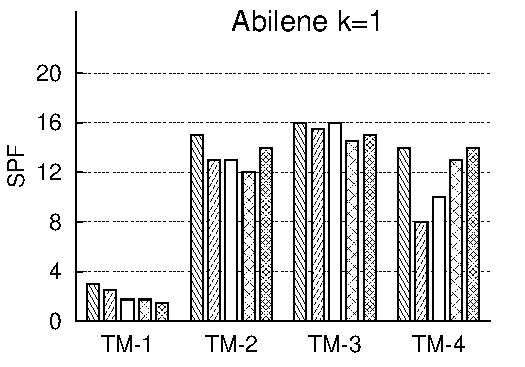
\includegraphics[scale=0.5]{final_images/G6_capacity/Abilene/k1_hist_plot.pdf}}
\subfigure{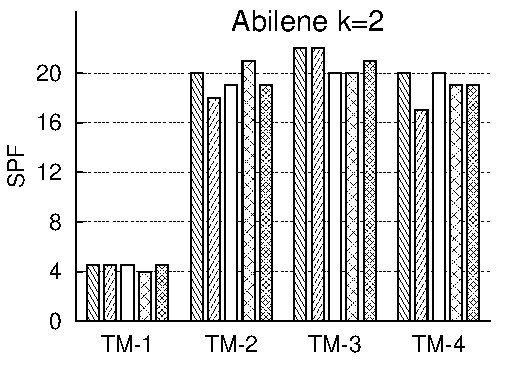
\includegraphics[scale=0.5]{final_images/G6_capacity/Abilene/k2_hist_plot.pdf}}
\subfigure{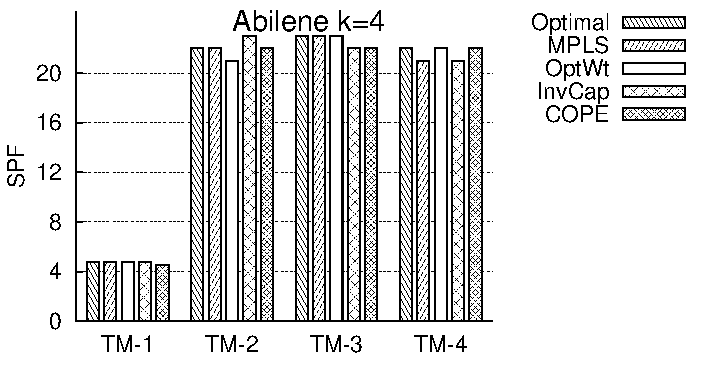
\includegraphics[scale=0.5]{final_images/G6_capacity/Abilene/k4_hist_plot.pdf}}
 \subfigure{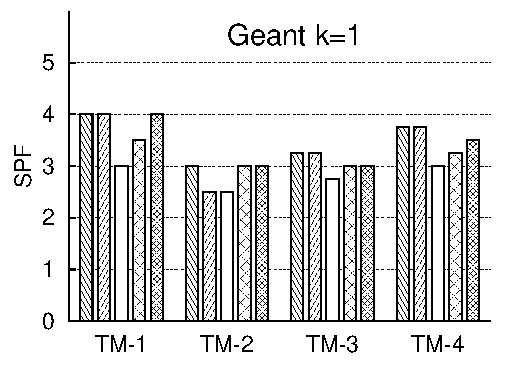
\includegraphics[scale=0.5]{final_images/G6_capacity/Geant/k1_hist_plot.pdf}}
 \subfigure{\includegraphics[scale=0.5]{final_images/G6_capacity/Geant/k2_hist_plot.pdf}}
 \subfigure{\includegraphics[scale=0.5]{final_images/G6_capacity/Geant/k4_hist_plot.pdf}}
\subfigure{\includegraphics[scale=0.5]{final_images/G6_capacity/USISP/k1_hist_plot.pdf}}
\subfigure{\includegraphics[scale=0.5]{final_images/G6_capacity/USISP/k2_hist_plot.pdf}}
\subfigure{\includegraphics[scale=0.5]{final_images/G6_capacity/USISP/k4_hist_plot.pdf}}
 \end{center}
\caption{\label{fig:capacity_diversity} Comparison of SPF among TE schemes for different levels of location diversity; SPF values are obtained using ns-2 simulations }
\vspace{-0.2in}
\end{figure*}

\subsection{Capacity increase with location diversity}
%
%We first present our results for the maximum capacity increase as calculated by the linear program in technical report \cite{TR}, and then as measured experimentally.

%\subsubsection{Theoretical capacity increase with location diversity}

%%\textbf{explaining the graph presented}

%In Figure~\ref{fig:capacity_opt}, we present the results for the maximum SPF using \opt{} and \invcap{} routing for the selected TMs. For each TM, the left bar shows the SPF  without location diversity ($k = 1$) and the right bar shows the SPF when a node can obtain content from all nodes in the network except itself ($k = n - 1$, $n  =$ number of nodes). Note that the later case is the maximum SPF which can be achieved with location diversity.

%%While \opt{} has the freedom to split flows arbitrarily among multiple locations and  to choose any routing, \invcap{} can split flows arbitrarily among multiple locations but is restricted to use the default shortest path routing. 

%%\textf{How linear program works}
%%The linear program works as follows: For every node pair ($i$,$j$) where $i$ is the source and $j$ is the destination, the original flow without location diversity is equal to the traffic matrix entry $f_{i,j}$.  We add $(k - 1)$ new sources randomly for this flow and solve the linear program which optimizes the MLU. If the optimal MLU obtained from the linear program is $\alpha$, then the capacity of the network is $1/\alpha$.  We increase the value of $k$ from 1 to $(n-1)$ where $n$ is the number of nodes in the network. The optimal routing can be achieved using $m$ locations, where $m \leq (n-1)$. 

%%\textbf{what is the capacity increase}

%The capacity increase in the network for \opt{} is  1.6$\times$ for Abilene,  1.2$\times$ for Geant and less than 1.1$\times$ for US-ISP topology. The capacity increase for \invcap{} is approx 2.1$\times$ for Abilene, 1.3$\times$ for Geant topology and 1.5$\times$ for US-ISP topology.  Clearly location diversity increases the capacity both for \opt{} and \invcap{} but the increase depends on the ISP topology and traffic matrix. \invcap{} has less capacity than \opt{} even with location diversity but the relative difference between the two has diminished. This result shows that location diversity reduces the difference in capacity among TE schemes.

%

%%\textbf{only few locations get max capacity increase}

%While $(n-1)$ locations can certainly give the maximum SPF, we find only 2-4 locations can give the maximum SPF for most matrices both for \invcap{} and \opt{}). The reason is that the immediate links to some nodes often become the bottleneck first. As each node in these ISP topologies typically has on average only a few incoming links (3-4 links), even a small number of additional locations suffice to saturate all incoming links for the most loaded node in the network.
%%traffic equally on all incoming links in the network. %Thus the network achieves the optimal MLU routing only with a small degree of location diversity.

%%\textbf{summary sentence}

%%Results from linear program solutions show that location diversity not only increases the capacity of the network but also reduces the difference in capacity among TE schemes.

%\subsubsection{Capacity increase for location diversity using ns-2 simulations}

%\textbf{why LP is not practical?}

%The capacity increase calculated above using a linear program may not be achievable in practice. There are two reasons for this. First, users in a network may not split their flows optimally among multiple locations as in the linear program solution. Second, the routes computed using any realistic TE scheme would in general be different from the optimal routing computed above. Nevertheless, we find that location diversity increases the capacity significantly for all TE schemes.

In Figure~\ref{fig:capacity_diversity}, we present the SPF values obtained using ns-2 simulations for the selected TMs. We compared all TE schemes for three levels of location diversity: $k = 1, 2$ and $4$.  Note that we do not present the results for \cope{} for US-ISP (k =2 and k = 4), since the implementation of \cope{}'s algorithm failed to compute a feasible set of routes even after 12 hours of simulation time (1 million iterations)  after which we aborted the simulation. We have used authors' implementation of the algorithm and communication with them confirmed that indeed in some cases \cope{}'s implementation can take a long time to terminate. This happens in cases where barrier-crossover method to solve a linear program fails and \cope\ instead uses simplex method which is much slower.


The average capacity increase for \opt{} from $k = 1$ to $k = 4$ is 1.41$\times$ and from $k = 1$ to $k = 2$ is 1.31$\times$. \opt{} is the maximum SPF for a network with no location diversity ($k = 1$). This shows that a network with location diversity of $k = 4$ has 40\% greater capacity than a network with no location diversity. Even location diversity of $k = 2$ gives $75\%$ of capacity increase obtained from location diversity of $k = 4$. 

%
%
%  \begin{tabular}{ p{1.8cm} | p{0.4cm} | p{0.4cm} | p{0.4cm}  | p{0.4cm}  }
%\hline
%TE/\opt{}&  k=1& k=2 & k=4 \\ \hline
%\opt{}/\opt{} & 1 (1) & 1 (1)  & 1(1)   \\ 
%\mplsavg{}/ \opt{} & 0.89 () & 98 & 0.99 \\
%\optwt{}/\opt{} & 0.73 & 0.99 & 0.99 \\
%\invcap{}/\opt{} & 0.91 & 0.86 & 0.85  \\
%\cope{}/\opt{} & 0.91 & 0.99  & 0.98 \\  \hline
%  \end{tabular}
%

%\begin{figure*}[tbh]

%\begin{minipage}{2in}\footnotesize
%\begin{center}
%  \begin{tabular}{ p{1.8cm} | p{0.4cm} | p{0.4cm} | p{0.4cm}  }
%\hline
%TE/\opt{}&  k=1  & k=2 & k=4 \\ \hline
%\opt{}/\opt{} & 1 & 1 & 1 \\ 
%\mplsavg{}/ \opt{} & 0.89 & 98 & 0.99 \\
%\optwt{}/\opt{} & 0.73 & 0.99 & 0.99 \\
%\invcap{}/\opt{} & 0.91 & 0.86 & 0.85  \\
%\cope{}/\opt{} & 0.91 & 0.99  & 0.98 \\  \hline
%  \end{tabular}
%\vspace{0.2in}
%  \caption{Comparison of SPF values}
%\vspace{-0.3in}
%  \label{fig:cap_comparison}
%\end{center}
%\end{minipage}
%\hspace{0.5cm}
%\begin{minipage}{2in}
%  \begin{center}
%\includegraphics[scale=0.6]{final_images/G11_div_nodiv/Geant_k4/Geant_k4.pdf}
%  \end{center}
%  \caption{Effect of partial location diversity for Geant TMs.}
%  \label{fig:capacity_fraction_diversity}
%\end{minipage}
%\hspace{0.5cm}
%\begin{minipage}{2in}
%  \begin{center}
%\includegraphics[scale=0.7]{final_images/Geant_TCP_points_plot.pdf}
%%\subfigure[UDP]{\label{fig:UDP_higher_loads}\includegraphics[scale=0.35]{final_images/UDP_higher_loads.png}}
%  \caption{TCP performance at increasing loads for Geant TM}
%\label{fig:TCP_higher_loads}
%  \end{center}
%%\label{fig:TCP_higher_loads}
%\end{minipage}
%\vspace{-0.2in}
%\end{figure*}




%\begin{figure}\footnotesize
%\begin{center}
%
%  \begin{tabular}{| l | c |  c | c |  c }
%\hline
%Routing / Routing &  k = 1  & k = 2 & k = 4 \\ \hline
%\opt{} / \opt{} & 1 & 1 & 1 \\ 
%\mplsavg{} / \opt{} & 0.89 & 98 & 0.99 \\
%\optwt{} / \opt{} & 0.73 & 0.99 & 0.99 \\
%\invcap{} / \opt{} & 0.91 & 0.86 & 0.85  \\
%\cope{} / \opt{} & 0.91 & 0.99  & 1.02 \\  \hline
%  \end{tabular}
%\vspace{0.2in}
%  \caption{Comparison of SPF values}
%\vspace{-0.3in}
%  \label{fig:cap_comparison}
%\end{center}
%\end{figure}

%\textbf{location diversity reduces TE differences}

%Over all TMs, \opt\ has 

%The maximum difference among \opt\ and other 


%Location diversity significantly reduces the difference in capacity among TE schemes. In fact, other TE schemes perform better than \opt\ in some cases. This is because location diversity changes the TM after optimal TE is implemented 
\begin{figure}\footnotesize
\centering
  \begin{tabular}{ l | c | c | c  }
%  \begin{tabular}{ p{1.8cm} | p{0.4cm} | p{0.4cm} | p{0.4cm}  }
TE/\opt{}&  k=1  & k=2 & k=4 \\ \hline
\opt{}/\opt{} & 1 & 1 & 1 \\ 
\mplsavg{}/ \opt{} & 0.89 & 0.98 & 0.99 \\
\optwt{}/\opt{} & 0.73 & 0.99 & 0.99 \\
\invcap{}/\opt{} & 0.91 & 0.86 & 0.85  \\
\cope{}/\opt{} & 0.91 & 0.99  & 0.98 \\  
  \end{tabular}
  \caption{Comparison of SPF values}
  \label{fig:cap_comparison}
\end{figure}
Location diversity enables all TE schemes to achieve near-optimal capacity. In Figure~\ref{fig:cap_comparison} we compare the SPF of \opt{} to that of other TE schemes. The statistic presented is ratio of SPF of TE scheme to SPF  of \opt{} for the same level of location diversity averaged over all TMs. Except \invcap{}, all TE schemes have SPF within 2\% of \opt\ for $k= 4$ as well as $k = 2$. Figure \ref{fig:capacity_diversity} shows that with location diversity any TE scheme has at most 10\% capacity difference compared to \opt. On average \invcap{} has 15\% less capacity compared to \opt{} for a location diversity of  $k = 4$.  In the worst case \invcap\ achieves a capacity that is 30\% less than \opt\ (Figure \ref{fig:capacity_diversity}, Geant k = 2).

%\begin{figure}\footnotesize
%  \begin{tabular}{ p{1.8cm} | p{0.4cm} | p{0.4cm} | p{0.4cm}  }
%\hline
%TE/\opt{}&  k=1  & k=2 & k=4 \\ \hline
%\opt{}/\opt{} & 1 & 1 & 1 \\ 
%\mplsavg{}/ \opt{} & 0.89 & 0.98 & 0.99 \\
%\optwt{}/\opt{} & 0.73 & 0.99 & 0.99 \\
%\invcap{}/\opt{} & 0.91 & 0.86 & 0.85  \\
%\cope{}/\opt{} & 0.91 & 0.99  & 0.98 \\  \hline
%  \end{tabular}
%  \caption{Comparison of SPF values}
%  \label{fig:cap_comparison}
%\end{figure}

The above result calls into question the usefulness of online TE schemes. In today's Internet, offline TE schemes such as \optwt{} or \mplsavg{} are commonly used. It is believed that these schemes are sub-optimal and online TE schemes (e.g., TeXCP, MATE etc.) can achieve near-optimal capacity.  However, our results suggest that application adaptation to location diversity results in near-optimal SPF for all TE schemes.  Even the shortest-path routing scheme, \optwt{}, achieves the same SPF as TE schemes employing MPLS for flow splitting.



%In contrast, without location diversity \opt{} has upto 2$\times$ higher capacity than \invcap{} for some TMs.

%In comparison without any location diversity, \opt\ has up to 2$\times$ more capacity than \invcap\ for some traffic matrices. 


%While \invcap\ reduces its relative capacity difference compared to \opt\, it still remains sub-optimal.
%Based on this, we conclude that although application adaptation significantly undermines the value of traffic engineering, it does not obviate it completely.

%On average \invcap{} has 85\% capacity compared to \opt{} even for a location diversity of $k = 4$.  \invcap{} is a simple static routing scheme which does not consider the traffic demand in the network while other TE schemes compute routing based on measured traffic demand. 

\subsubsection{Other results}
We briefly summarize other experimental results deferred to a technical report \cite{TR}. First, SPF increases in a concave manner with the fraction of traffic that can leverage location diversity. Even if only half of the traffic has location diversity, it suffices to capture over 90\% of the potential increase in SPF for each TE scheme, and the SPFs achieved by different TE schemes continues to be less that 5\%. Second, the ``near-optimality" of capacity  achieved by all TE schemes is reflected not only in their SPFs but in application performance metrics as well, i.e., TCP download rates and MOS scores (in the mean as well as across various percentiles) degrade similarly for all TE schemes as the demand approaches the SPF capacity point. As expected, application performance starts to dip earlier under \invcap\ as its SPF is somewhat lower than TE schemes. Thus, these results also suggest that, unlike link utilization metrics, SPF is a sound empirical metric to measure how effectively a TE scheme can accommodate load surges under location diversity.
 

%Thus, in addition to further substantiating our conclusions, these results also suggest that SPF is a sound empirical metric to capture the capacity increase as well as application performance  under load surges

%\subsection{Partial location diversity}

%Next, we consider a scenario where only a fraction of traffic can leverage location diversity, as is the case in today's Internet. The details of our experiment and the results are described in a technical report \cite{TR}. in this experiment, we vary the fraction of traffic with location diversity and measure SPF values. We observe that the curve of SPF vs fraction of traffic with location diversity shows a concave behavior.  Our primary finding from this experiment is that  all TE schemes get more than 90\% of  increase in SPF even when only 50\% traffic has location diversity.  Moreover, the difference in capacity among for TE schemes remains less than 5\% even when only half of the traffic can leverage location diversity.


%\textbf{section summary}

%In summary, we find that  application adaptation due to location diversity increases the capacity of the network by up to 1.4$\times$ compared to a network with no location diversity even with a small number of locations (k = 4).  Using a simple practical adaptation scheme such as parallel TCP downloads, we show that application level adaptation enables all engineering schemes to achieve near-optimal capacity. These results call into question the value of exploring online TE schemes for further improvement. 



%Our results in the previous section show that for internet traffic loads and traffic matrices the difference in MLU for TE schemes make little difference in application performance for different TE methods. The case for traffic engineering is made by proposing that when traffic demands scale in the future Optimal will be able to sustain a higher demand than a MLU suboptimal scheme \cite{TeXCP06}.



% simulate application adaptation the network capacity for ns-2 simulations when a file is downloaded in parallel from multiple locations.



% SIMULATING TM WITH LOCATION DIVERSITY


%The routing for a TM depends on other TMs in the dataset. We compute routing for T using a new set of TMs S' obtained from set S. 

%We compute the routing and we generate a file arrival sequence from the traffic matrix identical to single location download. But we choose ($k - 1$) additional source locations for each file. Then, we simulate parallel download of each file from k locations and measure the new traffic matrix. This gives an set of TMs S' which have adapted to location diversity in the network.


%For every TM in this set S, we compute its adapted version as follows: We compute the routing and we generate a file arrival sequence from the traffic matrix identical to single location download. But we choose ($k - 1$) additional source locations for each file. Then, we simulate parallel download of each file from k locations and measure the new traffic matrix. This gives an set of TMs S' which have adapted to location diversity in the network.


%For every TM T, routing depends on a subset of other TMs in the set S. For example for \opt{} routing depends on  current TM and for \optwt{} it depends on the average of past three hours TMs. 


%We can compute a routing for T based on set S, but it will be extremely inaccurate. This is because the T will change during the simulation due to parallel downloads. For example, \opt{} would compute the optimal routing for TM T, but we use this routing to simulate a different TM T'. Therefore, we are not simulating \opt{} routing for this TM. We 


%Which TMs it depends on depends on TE scheme.

% e.g., \opt{} routing depends on the current TM \optwt{}. We do not compute routing based on TM in set S. This is because we are going to simulate T with parallel download of each file 


%To compute routing for T, we obtain a new set of S' which have adapted to the location diversity in the network.




%\emph{First Step:} Let S be the original set of TMs in our dataset. For every TM in this set S, we compute its adapted version as follows: We compute the routing and we generate a file arrival sequence from the traffic matrix identical to single location download. But we choose ($k - 1$) additional source locations for each file. Then, we simulate parallel download of each file from k locations and measure the new traffic matrix. This gives an set of TMs S' which have adapted to location diversity in the network.


%As above, we generate a file arrival sequence for T and choose ($k - 1$) additional source locations for each file. Now we use the set of adapted TMs S' computed above to generate a routing for T.


%\emph{First Step:} Let S be the original set of TMs in our dataset. 

%For every TM in this set S, we compute its adapted version as follows: We compute the routing and we generate a file arrival sequence from the traffic matrix identical to single location download. But we choose ($k - 1$) additional source locations for each file. Then, we simulate parallel download of each file from k locations and measure the new traffic matrix. This gives an set of TMs S' which have adapted to location diversity in the network.

%\emph{Second Step:}  To simulate a TM with location diversity, we start with original TM T $\in$ S. As above, we generate a file arrival sequence for T and choose ($k - 1$) additional source locations for each file. Now we use the set of adapted TMs S' computed above to generate a routing for T.

%The important difference is that we compute routing for T based on the set of adapted TMs S'. Finally we simulate parallel download of each file using the routing computed for the set of adapted TMs.

%We compute a routing for T based on the new set of TMs S'.  As above, we generate a file arrival sequence for T and choose ($k - 1$) additional source locations for each file. We simulate parallel downloads but we use the routing computed using the new set of TMs S'. 


%Let T $\in$ S be the original TM we want to simulate with location diversity. We compute a routing for T based on the new set of TMs S'.  As above, we generate a file arrival sequence for T and choose ($k - 1$) additional source locations for each file. We simulate parallel downloads but we use the routing computed using the new set of TMs S'. 

%Since we are simulating a TM with diversity, it is more accurate to compute routing using the set of adapted TMs S' than the original TMs S. We believe this process ensures a fairer comparison of TE schemes.



%For \opt{}, we compute only the current TM with diversity; For \optwt{} and  \mplsavg{}, we compute the average of TMs in past 3 hours;  \optwt{} and  \mplsavg{} uses the average of past 3 hour TMs  and \cope{} uses all TMs from the previous day. If T is the metric we want to simulate, then in the first step we simulate the matrices that determine its routing. Therefore, for \opt{} we simulate the same matrix, for \mplsavg{} we simulate the average of past 3 hours traffic matrix, for \cope{} we simulate a subset of matrices from last day. \invcap{} does not need a simulation for first step since its routing is fixed. The second step is identical for all routing schemes: we compute the routing for T using the respective routing schemes based on simulated matrices in the first step. 

  

%\textbf{two steps of simulation}
%We solve this problem using a two step simulation process: 

%Suppose T is the original matrix that we need to simulate with location diversity; 'k' is the number of source locations each file; R is the TE scheme and S is the set of matrices based on which R computes routing for T.

%For every traffic matrix $S_i$ in set S we generate a traffic matrix $S'_i$ by doing parallel download of each file in traffic matrix $S_i$. 

%In first step, we translate this traffic matrix into a sequence of file downloads as described before. For every file being downloaded, we add k-1 new source nodes other than the original source node. In our simulations, each  file is downloaded in parallel from these k  locations. We measure the traffic matrix T1 resulting from simulation. It is expected that the resulting traffic matrix is different from T.   

%In the second step we compute a routing for T1.  We again simulate T with parallel downloads but we use the routing computed for T1. We expect that the resulting traffic matrix will be similar to T1. This is because in first step, when T is simulated with parallel downloads, it resulted in the traffic matrix T1. This process ensures that we simulate the traffic matrix with a routing which has been computed for that traffic matrix.

%\textbf{how is two steps better than single step}
%The merit of two steps of simulations is that in the second step we simulate an adapted traffic matrix with a routing which has been computed for a similar traffic matrix. We believe this process ensures a fair comparison of traffic engineering schemes. 

%\textbf{detail of simulation}
%Our simulation process depends on the traffic engineering scheme we want to simulate. This is because the set of TMs using which routing is computed depends on TE scheme, e.g.  \optwt{} uses the average of past 3 hour TMs  and \cope{} uses all TMs from the previous day. If T is the metric we want to simulate, then in the first step we simulate the matrices that determine its routing. Therefore, for \opt{} we simulate the same matrix, for \mplsavg{} we simulate the average of past 3 hours traffic matrix, for \cope{} we simulate a subset of matrices from last day. \invcap{} does not need a simulation for first step since its routing is fixed. The second step is identical for all routing schemes: we compute the routing for T using the respective routing schemes based on simulated matrices in the first step. 


%```````````````

%In this section, we present results from experiments which simulate application adaptation due to location diversity. We show that location diversity increases the capacity of ISP networks by up to more than 50\%. Surprisingly, it significantly reduces the difference between traffic engineering methods and nearly vanishes the advantage of optimal traffic engineering over other traffic engineering schemes in terms of capacity.

%Our results in the previous section show that for internet traffic loads and traffic matrices the difference in MLU for TE schemes make little difference in application performance for different TE methods. The case for traffic engineering is made by proposing that when traffic demands scale in the future Optimal will be able to sustain a higher demand than a MLU suboptimal scheme \cite{TeXCP06}.

%We take a different stance on the question of capacity. Our stance is based on the observation that a significant fraction of internet traffic has location diversity available to it.

%Optimal exploits path diversity in the network to increase its capacity. Location diversity also increases capacity of the network by giving multiple locations for each download. Importantly, this capacity increase is available to all TE schemes. We experimentally compare of TE schemes with location diversity and show that the the differences in capacity between TE schemes vanish even when a small number of locations are available for file download.

%```````````````

%We take a different stance on the question of capacity. Our stance is based on the observation that a significant fraction of internet traffic has location diversity available to it.

%Optimal exploits path diversity in the network to increase its capacity. Location diversity also increases capacity of the network by giving multiple locations for each download. Importantly, this capacity increase is available to all TE schemes. We experimentally compare of TE schemes with location diversity and show that the the differences in capacity between TE schemes vanish even when a small number of locations are available for file download.

%\subsubsection{Definition of the capacity of a network}

%In line with the theme of the paper, we define the capacity of a network in terms of the file download rates. 

%We call the internet TM to be a load 1.0 and TM at load $x$ is obtained by multiplying the internet TM by $x$. On increasing the load, some links in the network reach utilization of close to 1. If the traffic on a link in the network nears the capacity then the download rate of files through that link must reduce.  Experimentally we observe that as we increase the load on the network, the lower percentile of file download rate (e.g. 10th percentile, 20th percentile) reduces sharply. Hence, we infer that a sharp drop in file download rate is because the network is reaching capacity on one or more links. This leads to our definition of capacity:

%\emph{The capacity of a network is the least load at which the 10th percentile download rate is less than 100KBps.}

%Our rationale for selecting the 10th percentile is that a value lower than 10th percentile is prone to artifacts from our simulation.  For example, the 5th percentile download rate is small even at load = 1.0  since 5\% of internet users in US have access link less than 256Kbps. We selected 100KBps as the threshold but the comparative results for TE methods remained same for a range of values from 75KBps to 125 KBps. The capacity of TE methods measured using our capacity metric follows the same order as that predicted using theoretical MLU. The load at which capacity is reached according to our definition is approximately is  15\%-20\% less than the load at which theoretical MLU touches 1.

%In fig ~\ref{fig:10th_percentile_TMs} we plot the 10th percentile throughputs for 3 TMs from Abilene, Geant and US-ISP. The drop in 10th percentile throughput as load on the network increases can be seen in all three graphs. 100 KBps lies in the region of a sharp drop in throuhgput which makes it a good choice for selecting as a thresold value.

%Other contenders for the capacity metric from our experiment such as the file download times and the maximum link utilization did not show a distinct value which could be unambiguously selected as the capacity point. For example MLU increased and decreased on small variations in load. The total file download times became infinite much before MLU became 1 because of zero download rates for some files.

%\subsection{Capacity without traffic with diversity }

%We randomly selected 5 TMs from Abilene, Geant and US-ISP datasets. For each TM we computed the capacity for each routing and the ratio of its capacity compared to OPTIMAL. We call this ratio the \emph{capacity ratio} for a routing. In fig \ref{fig:all_isps_capacity_without_diversity} we plot the average capacity ratio for 5 TMs based on our capacity metric in fig ~\ref{fig:capacity_ratio_no_diversity} and using theoretical MLU values in fig ~\ref{fig:capacity_ratio_no_diversity_MLU}. The figures show that capacity ratio for our metric correlates well with the MLU predicted capacity ratio but is 15-20\% higher for some same.

%In fig ~\ref{fig:capacity_ratio_no_diversity} Optimal clearly has a higher capacity than other schemes. For Abilene, shortest path routing methods (InvCap, OspfOptWt) can only achieve  65-70\% of the capacity of Optimal and for US-ISP they have a capacity of 70-85\%. Offline TE schemes which use MPLS (MplsAvg,COPE) have a higher capacity than shortest path routing methods and can achieve more than 90\% of the capacity of Optimal in Geant and  US-ISP toplogies but for Abilene they have 75-85\% capacity of Optimal. The anomaly that the capacity COPE has a higher capacity than Optimal  for Geant topology is becuase we do not simulate the traffic matrix accurately. As mentioned earlier, the link utilization in our simulation can be 0.1 different from the link utilization expected using calculations. 

%Without diversity, Optimal enjoys a capacity advantage over offline TE schemes especially shortest path routing schemes.  OspfOptWt is a widely used traffic engineering scheme in the internet. Its lower capacity should motivate a switch to a higher capacity traffic engineering scheme either based on offline MPLS based scheme or online TE. But, our results in the following section shw that effect of location diversity vanishes the capacity difference between OspfOptWt and Optimal.

%It has a higher capacity than other TE scheme by upto 25\%.  MLU Optimal has an advantage over traffic engineering schemes in terms of capacity. MLU Optimal has 25\% higher capacity than other traffic engineering schemes for Abilene topology. In Geant, the capacity predicted for COPE is higher than MLU optimal. We take it to be an error in our simulation. The link utilization we simulate in ns-2 and the actual link utilizations differ upto 0.1. On average OSPFOptWt performs worst in terms of capacity in our simulations. OSPFOptWt is a widely used traffic engineering scheme in the internet. Its poor performance should motivate a switch to a higher capacity traffic engineering scheme.But, our results in the following section suggest that effect of location diversity increases the capacity for OSPFOptWt similar to even MLUOptimalScheme.
%
%\begin{figure*}[tbh]
%  \begin{center}
% \subfigure[ Capacity ratio using ns simulations]{\label{fig:capacity_ratio_no_diversity}\includegraphics[scale=0.65]{newImages/Capacity/cap_without_diversity/capacity_without_diversity.jpg}}
%\subfigure[Capacity ratio predicted using MLU]{\label{fig:capacity_ratio_no_diversity_MLU}\includegraphics[scale=0.65]{newImages/Capacity/cap_without_diversity/capacity_theoretical.jpg}}
%  \end{center}
%  \caption{Capacity of TE schemes without diversity}
%  \label{fig:all_isps_capacity_without_diversity}
%\end{figure*}

%\begin{figure*}[htb]
%  \begin{center} \subfigure[US-ISP TM]{\includegraphics[scale=0.75]{newImages/ATT_download_rate_percentiles_10_plot.pdf}}
%\subfigure[Geant TM]{\includegraphics[scale=0.75]{newImages/Geant_download_rate_percentiles_10_plot.pdf}}
%\subfigure[Abilene TM]{\includegraphics[scale=0.75]{newImages/Abilene_download_rate_percentiles_10_plot.pdf}}
%  \end{center}
%  \caption{10th percentile throughput with increasing loads for TMs}
%  \label{fig:10th_percentile_TMs}
%\end{figure*}

%\subsection{Capacity with diversity}

%We compare the capacity of TE schmes under diversity using two approaches. 1. Sampling the throughputs from multiple locations. 2. Simulating a traffic matrix with parallel downloads.

%\subsubsection{Experiment description}

%\subsubsection{Results}

%We compare the capacity of TE schemes with location diversity in fig ~\ref{fig:all_isps_capacity_with_diversity}. In fig ~\ref{fig:capacity_with_diversity} we plot the capacity with diversity for 3 ISPs. Surprisingly, all TE schemes (except InvCap) have the same capacity after diversity in all 3 ISPs. The capacity of offline TE schemes using MPLS and even OspfOptWt has the same capacity as Optimal. InvCap still has upto 30\% less capacity than Optimal. Less powerful TE schemes such as OspfOptWt leverage location diversity  to reach the capacity of Optimal but a simple static routing scheme such as InvCap is not enough to harness the benefits of location diversity. OspfOptWt is a widely used intra-domain routing protocol. Our results show if application can leverage location diversity, ISPs can continue to use existing intra-domain routing protocols and achieve capacity close to Optimal scheme.

%We earlier made the case that location diversity can increase capacity in ISP networks. In fig ~\ref{fig:capacity_inc_with_diversity} we plot the capacity increase measured in our experiments. The results are the average of the ratio of capacity increase for 5 TMs.
%Concurrent with our findings in ~\ref{fig:capacity_ratio_no_diversity} and ~\ref{fig:capacity_with_diversity} , we see that the capacity of OspfOptWt increases maximum in all 3 ISPs - 2.2 $\times$ in Abilene, 2 $\times$ in Geant and 1.5 $\times$ in US-ISP respectively. The capacity for Optimal also increases 1.2-1.5$\times$, but the capacity increase works to the advatange of offline TE schemes and they reach the capacity for Optimal. InvCap also increases its capacity 1.2-2$\times$, but despite this increase other schemes still have a greater capacity.

%\begin{figure*}[tbh]
%  \begin{center}
% \subfigure[ Capacity ratio with diversity]{\label{fig:capacity_with_diversity}\includegraphics[scale=0.65]{newImages/Capacity/cap_with_diversity/capacity_with_diversity.jpg}}
%\subfigure[Capacity increase with diversity]{\label{fig:capacity_inc_with_diversity}\includegraphics[scale=0.65]{newImages/Capacity/cap_with_diversity/capacity_inc_with_diversity.jpg}}
%  \end{center}
%  \caption{Capacity of TE schemes with diversity}
%  \label{fig:all_isps_capacity_with_diversity}
%\end{figure*}

%\subsection{Application performance at higher surge factors}


%The near-optimality of the capacity of all TE schemes is reflected in application performance metrics as well.  Due to sub-optimal capacity of \invcap\ for some TMs, it shows a sub-optimal application performance for these TMs. The relevant graphs are presented in a technical report due to lack of space \cite{TR}. In our analysis, we compare different TE schemes at increasing surge factor for each TM based on application performance metrics - TCP download rate, MOS. We select different percentiles as well as the mean of the distribution of TCP download rate and MOS. As expected, we observe that application performance shows a decline as the surge factor increases towards the SPF value of the TE scheme for a TM. Notably, we do not find any significant difference in application performance of TE schemes irrespective of the statistic we use for comparison. For the TMs where SPF of \invcap\ is sub-optimal, its application performance is worse in comparison to other TE schemes for the same surge factor. 

%
%\begin{figure}[tbh]
%  \begin{center}
%\subfigure[TCP]{\label{fig:TCP_higher_loads}\includegraphics[scale=0.7]{final_images/TCP_higher_loads.png}}
%\subfigure[UDP]{\label{fig:UDP_higher_loads}\includegraphics[scale=0.7]{final_images/UDP_higher_loads.png}}
%  \end{center}
%  \caption{TCP and UDP performance at increasing loads for Geant TM}
%\label{fig:higher_loads}
%\end{figure}

% NOTE : Figure moved to previous section

%
%Figure \ref{fig:TCP_higher_loads} shows the 10th percentile of the download throughput distribution at different loads.   All TE schemes have near identical values  except \invcap. The horizontal distance between the curve of \invcap\ and that of other TE schemes curves is approximately equal to the difference in SPF values between them which is indicative of capacity difference between them. Other statistics, e.g. mean, median show similar trends but the horizontal distance between the curve for \invcap\ and other TE schemes reduces at higher percentile values. 

%

%We compute MOS scores for all source-destination pairs as in Section~\ref{sec:UDP_perf}. We find the distribution of MOS scores by selecting node pairs randomly but giving more weight to pairs with more traffic between them. This distribution shows similar trends as the distribution of download throughputs. We do not present the graph due to lack of space. All TE schemes have no significant difference in performance for VoIP traffic based on MOS scores, except \invcap\ which has lower performance at loads near SPF. Note that a VoIP call is a single UDP connection between source and destination nodes without any location diversity, but it still benefits from the rest of the traffic being able to leverage location diversity. 


%We compute MOS scores for source-destination pairs as in Section~\ref{sec:UDP_perf}.  We plot the distribution of MOS scores by selecting node pairs randomly but giving more weight to pairs with more traffic between them. All TE schemes show nearly same performance for VoIP traffic as well. Note that a VoIP call is a singe UDP connection between source and destination nodes without any location diversity, but it still benefits from the rest of the traffic being able to leverage location diversity.


%The curve for UDP shows a similar behavior 

%\textbf{UDP traffic}
%Figure~\ref{fig:UDP_higher_loads}  shows the 10th percentile value of MOS-score distribution at different loads. We compute MOS scores for source-destination pairs as in Section~\ref{sec:UDP_perf}.  We plot the distribution of MOS scores by selecting node pairs randomly but giving more weight to pairs with more traffic between them. All TE schemes show nearly same performance for VoIP traffic as well. Note that a VoIP call is a singe UDP connection between source and destination nodes without any location diversity, but it still benefits from the rest of the traffic being able to leverage location diversity.

\subsection{Experiments with least latency adaptation}
\label{sec:leastlatency}
%Internet users often leverage location diversity by downloading a file from the closest location it is available. 
%For example, CDNs direct users to the least latency server location, and users choose nearby  mirror sites for file download.


In experiments until now, users leverage location diversity by downloading a file in parallel from all locations. Next, we present our experiment with least latency adaptation in which a user downloads a file from the closest location it is available. 
This adaptation is inspired by redirection schemes that are widely used by CDNs today \cite{Akamai2002,donar}.
These experiments reinforce our earlier finding that all TE schemes achieve nearly the same SPF values when applications adapt to location diversity.
With least latency adaptation, an increase in location diversity yields little improvement in SPF of any TE scheme.
This adaptation reduces the SPF of \opt\ to bridge the gap between \opt\ and sub-optimal schemes such as \optwt.




\eat
{
Real-world systems especially CDNs \cite{Akamai2002,donar} use various forms of this adaptation account for  server load, datacenter bandwidth, round trip delay, network loss rates, billing costs at each server deployment, and so on \cite{Akamai2002,donar}.


In experiments in Section \ref{sec:capacity}, users leverage location diversity by downloading a file in parallel from all locations.
Another common approach to leverage location diversity is to download a file from the closest location it is available.
Real-world systems use various forms of this adaptation, which we call \emph{least latency adaptation}. 
These adaptations account for  server load, datacenter bandwidth, round trip delay, network loss rates, billing costs at each server deployment, and so on \cite{Akamai2002,donar}.


Accurately modeling all these factors is a complex problem, and is beyond the scope of this work.
}

%In Section \ref{sec:capacity}, users download a file from all locations the file is available using parallel TCP connections.
%In this section, we experiment with another common approach to leverage location diversity - 
%a user downloads a file from the closest location it is available. 
%In general, real-world systems use various forms of \emph{least latency adaptation} accounting for  server load, datacenter bandwidth, round trip latency, network loss rates, billing costs at each server deployments, and so on \cite{Akamai2002,donar}.
%Accurately modeling all these factors is a complex problem, and is beyond the scope of this work.


%In the previous section, users downloaded a file from all locations the file is available using parallel TCP connections. 
%In this section, we experiment with another common approach to leverage location diversity - 
%a user downloads a file from the closest location it is available. 
%The distance between the user and the file location is measured as the propagation delay along the path between them.
%If there are multiple paths between two locations, we measure propagation delay as the weighted average of latencies of all paths; 
%the weight of a path is equal to the fraction of traffic it carries from source to the destination node.  
%This adaptation is called the least latency adaptation.

%However, least latency adaptation that we consider does not depend on the congestion in the network, i.e., the user chooses the same (closest) replica irrespective of the congestion on the path from that replica to the user.

%We seek to answer two main questions through our experiments with least latency adaptation.  
%As before, we vary the location diversity for each file keeping the total traffic requested by each node unchanged.
%First, we ask whether the effective capacity of the network to tolerate surges in traffic demand increases with location diversity.
%Second, we compare the relative performance of TE schemes accounting for location diversity.  
%We use SPF metric to compare TE schemes.


%We use  flow-level simulations instead of  packet level simulations for this set of experiments. Flow-level simulations are two  orders of magnitude faster than packet level simulations (few hundred seconds vs. few hours).  Moreover, flow-level simulations suffice to measure the  traffic between any two PoPs in this experiment. In comparison, our earlier experiments with parallel downloads required packet-level simulations to measure PoP-to-PoP traffic. This difference arises because least latency adaptation allows a user to download each file from one location only but a user downloads a fraction of a file from every location in case of  parallel downloads. In the latter case,  these fractions can only be estimated if the TCP throughputs of all connections are known; accurate estimation of TCP throughputs requires packet-level simulations. WIth least latency adaptation, flow-level simulations calculate the sum of sizes of files downloaded  at a PoP from any other PoP.

\subsubsection{Experiment procedure}


We model least latency adaptation as follows: a user downloads a file from the location that has the smallest propagation delay.
If there are multiple paths between two locations, propagation delay is measured as the weighted average of latencies of all paths; 
the weight of a path is equal to the fraction of traffic it carries.
To emulate a location diversity of $k$, each file is replicated at the original location based on traffic matrix and at $(k-1)$ additional locations. 
We select additional locations such that the probability of replicating a file at a location is proportional to its total outgoing link capacity. 
%Which location a user downloads a file from depends on two factors. 
%First, on the set of locations at which a file is available. 
%Second, on the routing in the network, which affects the propagation delay of paths. 


%Each file is replicated at the original location based on traffic matrix and at $(k-1)$ additional locations.  We select additional replica locations of a file such that the probability of placing a replica at a location is proportional to its total outgoing link capacity. 

%\subsubsection{Flow-level simulations}

We use  flow-level simulations instead of  packet level simulations for this set of experiments. 
Flow-level simulations are two  orders of magnitude faster than packet-level simulations (few hundred seconds vs. few hours).  
Moreover, flow-level simulations suffice to measure SPF in this experiment. 
Our earlier experiments with parallel downloads require packet-level simulations to measure PoP-to-PoP traffic, and hence SPF.
In case of  parallel downloads, a user downloads fractions of a file from multiple locations.
The fractions of a file downloaded from all locations can only be estimated if TCP throughput of every connection is known. 
We use packet-level simulations to accurately estimate TCP throughput in the earlier experiment.

%To accurately estimate TCP throughput of every connection, we use packet-level simulations.


%In this experiment, flow-level simulations calculate PoP-to-PoP traffic as follows.
%The incoming traffic rate at a PoP from any other PoP,  is calculated as the sum of sizes of files requested at this PoP from another PoP divided by the experiment duration.
%
%
%As before, we compute SPF for multiple levels of location diversity (k = 1, 3, 5 and 7). 
%We select additional replica locations of a file such that the probability of placing a replica at a location is proportional to its total outgoing link capacity. 



%SPF computation is straight forward once link utilizations are computed. 
%We increase the surge factor  for a TM in small increments as before and measure the MLU at every step. 
%The surge factor at which the MLU exceeds one is the SPF. 


%Multiplying the fraction of flows between the PoPs that cross a link by the PoP-to-PoP traffic, gives 
%Next, we calculate the fraction of this traffic that crosses a link, which is equal to the fraction of flows between the PoPs that cross the link.
%Given the traffic between two PoPs, we calculate the traffic on each link as the fraction of flows between the PoPs that cross this link.
%The total traffic on a link is calculated as the sum of PoP-to-PoP traffic that crosses this link for all pairs of PoPs. 


%Our flow-level simulations calculate PoP-to-PoP traffic by the sum of sizes of files requested at the destination PoP from the source PoP divided by the experiment duration.
%The incoming traffic rate at a PoP from any other PoP,  is calculated as the sum of sizes of files requested at this PoP from another PoP divided by the experiment duration.

To calculate SPF, flow level simulations measure PoP-to-PoP traffic and link utilizations.
PoP-to-PoP traffic (in bits/sec) is equal the sum of sizes of files requested at the sink PoP from another PoP divided by the experiment duration.
For a pair of PoPs, the PoP-to-PoP traffic crossing a link is equal to the fraction of flows between the PoPs that cross this link times the PoP-to-PoP traffic.
Summing the PoP-to-PoP traffic that crosses a link for all pairs of PoPs gives the total traffic on a link, which yields link utilization.
We increase the surge factor  for a TM in small increments as before. The least surge factor at which any link utilization exceeds 1 is the SPF.

%
%incoming traffic rate at a PoP from any other PoP  is calculated as the sum of sizes of files requested at this PoP from another PoP divided by the experiment duration.
%For a pair of PoPs, the PoP-to-PoP traffic crossing a link is equal to the fraction of flows between the PoPs that cross this link times the PoP-to-PoP traffic.
%Summing the PoP-to-PoP traffic that crosses a link for all pairs of PoPs gives the total traffic on a link, which yields link utilization.


%SPF computation is straight forward once link utilizations are computed. 
%We increase the surge factor  for a TM in small increments as before. The least surge factor at which traffic on a link exceeds capacity is the SPF.
%We compute SPF for multiple levels of location diversity (k = 1, 3, 5 and 7). 
%We select additional replica locations of a file such that the probability of placing a replica at a location is proportional to its total outgoing link capacity. 

\eat{
SPF computation is straight forward once link utilizations are computed. 
We increase the surge factor  for a TM in small increments as before and measure the MLU at every step. 
The surge factor at which the MLU exceeds one is the SPF. 
We compute SPF for multiple levels of location diversity (k = 1, 3, 5 and 7). 
We select additional replica locations of a file such that the probability of placing a replica at a location is proportional to its total outgoing link capacity. 
}

%As before, we vary the location diversity for each file keeping the total traffic requested by each node unchanged. We select additional replica locations such that the probability of placing a replica at a node is proportional to its total outgoing link capacity. 

%The locations of the replicas of a file influences traffic demand patterns, which affects the SPF metric. We experiment with two replica selection strategies. First, we place replicas at randomly selected nodes. Second, we place replicas such that the probability of placing the replica at a node is proportional to the sum of its outgoing links capacities. In both cases, no two replicas are placed at the same node. TBD: Do we need this.



\begin{figure}[t] 
\begin{center} 
\subfigure{\includegraphics[scale=0.5]{newimages/ATT2/k1_MLU.pdf}}
\subfigure{\includegraphics[scale=0.5]{newimages/ATT2/k3_MLU.pdf}}
\subfigure{\includegraphics[scale=0.5]{newimages/ATT2/k5_MLU.pdf}}
\subfigure{\includegraphics[scale=0.5]{newimages/ATT2/k7_MLU.pdf}}
 \end{center}
 \vspace{-0.2in}
\caption{[US-ISP] Mean SPF values of TE schemes with least latency adaptation. Error bars show the maximum and minimum SPF values over 20 repetitions. At higher location diversity, SPF values do not increase, in some cases even reduce, as location diversity increases from k = 1 to k = 7.}
\vspace{-0.2in}
\label{fig:leastlatspf}
\end{figure}


\begin{figure}[t] 
\begin{center}
\includegraphics[scale=0.5]{newimages/ATT2/TM27_totalTraffic.pdf}
\end{center}
\vspace{-0.2in}
\caption{[US-ISP, Traffic matrix TM-1, surge factor = 1]  Due to least latency adaptation, total traffic reduces to one-third as location diversity increases from k = 1 to k = 7.  Despite reduction in total traffic, SPF does not improve.}
\vspace{-0.2in}
\label{fig:totaltraffic}
\end{figure}



\subsubsection{Results}


We discuss here the results for the Tier-1 US ISP network. 
The Abilene and Geant topologies show qualitatively similar conclusions.
Figure \ref{fig:leastlatspf} shows the SPF values for four traffic matrices (same TMs as in Figure \ref{fig:capacity_diversity}). 
Location diversity increases from the top  graph (k = 1)  to the bottom graph (k = 7).
In a network with location diversity  (k = 3, 5, 7), all schemes including \opt\ have nearly same SPF values.
In comparison, \opt\ has higher SPF than other schemes in the absence of location diversity (k = 1). 
Even a static routing scheme, \invcap\ is at most 20\% worse compared to \opt.
In our experiments with the Abilene and Geant topologies, \invcap\ is at most 30\% worse compared to \opt. 
These observations are consistent with our findings in earlier set of experiments with parallel downloads.



%\opt\ has higher SPF than other schemes in the absence of location diversity (Figure 14, k = 1).
%In a network with location diversity  (k = 3, 5, 7), all schemes including \opt\ have nearly same SPF values. 
%Even a static routing scheme, \invcap\ is at most 20\% worse compared to \opt.
%In our experiments with the Abilene and Geant topologies, \invcap\ is at most 30\% worse compared to \opt. 
%In Section \ref{sec:capacity}, we found that application adaptation to location diversity reduces the difference between ``no TE'', i.e., \invcap\ and schemes that engineer traffic such as \opt. 
%Further, which TE scheme is used makes little difference to SPF.
%Our experiments with least latency adaptation reinforces both these findings.

Contrary to expectation, increasing location diversity yields little improvement in SPF of any TE scheme.
In Figure \ref{fig:leastlatspf}, the bars for each TM in the top graph (k = 1) are nearly as  tall as the bars in the bottom graph (k = 7). 
In some cases, bars in the bottom graph are slightly shorter, that is, SPF worsens on increasing location diversity, e.g.,  TM-2 for \opt.


With more location diversity, the utilization  of most links reduces dramatically.
This is evident from Figure 15, which shows the total traffic on all links at different levels of location diversity for a US-ISP  traffic matrix.
The total traffic on all links at k = 7 is one-third of the total traffic at k = 1 for every scheme.
But the peak link utilization does not reduce, it even increases in some cases, as location diversity increases.
This is why SPF does not improve despite a reduction in total traffic. 

Contrary to expectation, SPF yields no improvement with increasing location diversity.
In Figure \ref{fig:leastlatspf}, the bars for each TM in the top graph (k = 1) are nearly as  tall as the bars in the bottom graph (k = 7). 
In some cases, bars in the bottom graph are slightly shorter, that is, SPF worsens on increasing location diversity, e.g.,  TM-2 for \opt.


Figure 15 shows the total traffic on all links at different levels of location diversity for a US-ISP  traffic matrix. In this graph, the surge factor is always equal to 1, so the aggregate demand at end-nodes remains the same. But, the total traffic on all links at k = 7 is one-third of the total traffic at k = 1 for every scheme.

%For a single traffic matrix (TM-1), Figure \ref{fig:totaltraffic} shows the total traffic on all links for all location diversity levels. 

%On the other hand, the total traffic on all links  reduces to one-third for all TE schemes as location diversity increases from k = 1 to k = 7 (Figure \ref{fig:totaltraffic}). 
With more location diversity, users, on average, download files from a location closer than before.
This reduces the total traffic on all links, and reduces utilization of most links.
But the maximum link utilization does not reduce, it even increases in some cases, as location diversity increases. 
The most utilized link is the first to experience congestion at higher surge factors.
Least latency adaptation does not respond to congestion by moving traffic from the most utilized link to other under-utilized links.
It always downloads from the least propagation delay location, irrespective of the congestion on the path from that location.
This is why SPF does not improve despite a reduction in total traffic. 
An implication of this finding is that an adaptation scheme must be responsive to network congestion to leverage location diversity and increase the network's tolerance to traffic demand surges.



%Figure 15 shows a different metric: the total traffic on all links at different levels of location diversity for a US-ISP  traffic matrix.
%In this graph, the surge factor is always equal to 1, so the aggregate demand at end-nodes remains the same. 
%But, the total traffic on all links at k = 7 is one-third of the total traffic at k = 1 for every scheme.

%Figure 15 shows the total traffic on all links at different levels of location diversity for a US-ISP  traffic matrix. 
%In this graph, the surge factor is always equal to 1, so the aggregate demand at end-nodes remains the same. 
%But, the total traffic on all links at k = 7 is one-third of the total traffic at k = 1 for every scheme.

%For a single traffic matrix (TM-1), Figure \ref{fig:totaltraffic} shows the total traffic on all links for all location diversity levels. 

%On the other hand, the total traffic on all links  reduces to one-third for all TE schemes as location diversity increases from k = 1 to k = 7 (Figure \ref{fig:totaltraffic}). 
%With more location diversity, users, on average, download files from a location closer than before. 
%This is evident from Figure 15, which shows the total traffic on all links at different levels of location diversity for a US-ISP  traffic matrix.
%The total traffic on all links at k = 7 is one-third of the total traffic at k = 1 for every scheme.
%Increase in location diversity reduces utilization of most links.
%But the maximum link utilization does not reduce, it even increases in some cases, as location diversity increases. 
%The most utilized link is the first to experience congestion at higher surge factors.

Least latency adaptation does not respond to congestion by moving traffic from the most utilized link to other under-utilized links.
It always downloads from the least propagation delay location, irrespective of the congestion on the path from that location.
An implication of this finding is that an adaptation scheme must be responsive to network congestion to leverage location diversity and increase the network's tolerance to traffic demand surges.

%Location diversity blurs differences between TE schemes.





\eat{

We discuss here the results for the Tier-1 US ISP network. 
The Abilene and Geant topologies show qualitatively similar conclusions.
Figure \ref{fig:leastlatspf} shows the SPF values for four traffic matrices (same TMs as in Figure \ref{fig:capacity_diversity}). 
Location diversity increases from the top  graph (k = 1)  to the bottom graph (k = 7).
Contrary to expectation, SPF yields no improvement with increasing location diversity.
In Figure \ref{fig:leastlatspf}, the bars for each TM in the top graph (k = 1) are nearly as  tall as the bars in the bottom graph (k = 7). 
In some cases, bars in the bottom graph are slightly shorter, that is, SPF worsens on increasing location diversity, e.g.,  TM-2 for \opt. 
Figure 15 shows the total traffic on all links at different levels of location diversity for a US-ISP  traffic matrix. In this graph, the surge factor is always equal to 1, so the aggregate demand at end-nodes remains the same. But, the total traffic on all links at k = 7 is one-third of the total traffic at k = 1 for every scheme.

%For a single traffic matrix (TM-1), Figure \ref{fig:totaltraffic} shows the total traffic on all links for all location diversity levels. 

%On the other hand, the total traffic on all links  reduces to one-third for all TE schemes as location diversity increases from k = 1 to k = 7 (Figure \ref{fig:totaltraffic}). 
With more location diversity, users, on average, download files from a location closer than before.
This reduces the total traffic on all links, and reduces utilization of most links.
But the maximum link utilization does not reduce, it even increases in some cases, as location diversity increases. 
The most utilized link is the first to experience congestion at higher surge factors.
Least latency adaptation does not respond to congestion by moving traffic from the most utilized link to other under-utilized links.
It always downloads from the least propagation delay location, irrespective of the congestion on the path from that location.
This is why SPF does not improve despite a reduction in total traffic. 
An implication of this finding is that an adaptation scheme must be responsive to network congestion to leverage location diversity and increase the network's tolerance to traffic demand surges.

%Location diversity blurs differences between TE schemes.


\opt\ has higher SPF than other schemes in the absence of location diversity (Figure 14, k = 1).
In a network with location diversity  (k = 3, 5, 7), all schemes including \opt\ have nearly same SPF values. 
Even a static routing scheme, \invcap\ is at most 20\% worse compared to \opt.
In our experiments with the Abilene and Geant topologies, \invcap\ is at most 30\% worse compared to \opt. 
In Section \ref{sec:capacity}, we found that application adaptation to location diversity reduces the difference between ``no TE'', i.e., \invcap\ and schemes that engineer traffic such as \opt. 
Further, which TE scheme is used makes little difference to SPF.
Our experiments with least latency adaptation reinforces both these findings.

}


%TBD: Why variances so high?
%TBD: In another experiment, we place replicas at randomly selected nodes. However our results remain unchanged.

%Our experiments with least latency adaptation reinforce our earlier finding that application adaptation to location diversity reduces the difference between ``no TE'', i.e., \invcap\ and schemes that engineer traffic such as \opt.  
%Further, which TE scheme is used makes little difference to SPF.

%These experiment also show the SPF may not improve even with a higher location diversity unless the adaptation scheme is responsive to network congestion, e.g. the adaptation scheme of parallel TCP downloads,  to 


%TBD: Why variances so high?
%
%TBD: Conclusions here.

%\section{Discussion}
\label{sec:discuss}

\noindent\textbf{Limitations of our study:} We now point out the limitations of our work considering both the experiment design as well as evaluation objectives.

\noindent{\emph{Traffic engineering:}}
The TE problem for ISPs has other objectives as well, e.g., reducing interdomain traffic costs, computing backup routes for link failures,  ensuring QoS for different classes of traffic \cite{RFC3272} which we do not compare in our current study. We plan to include them in future work. 

\noindent{\emph{Network topology and traffic matrices:}}
 We perform experiments based on dataset from three ISPs and we experiment with a small set of TMs given our resources. Our simulation setup approximates or ignores some real world network topology entities such as multi-Gigabit backbone links, the router software/hardware at backbone and access links, TCP/IP software used at users and servers, to name a few.  We also do not model all aspects of Internet traffic demand pattern such as interdomain traffic, different variety of application layer protocols (HTTP, FTP, ICMP etc.), and the pattern of usage of these protocols.

\noindent{\emph{Location diversity:}}
 Without knowledge of future traffic matrices, our analysis considers only the uniform scaling of traffic matrices. Our capacity metric SPF and well as the MLU metric are based on this assumption. We show results using the adaptation scheme of parallel downloads of each file.  Accurately quantifying the capacity for TE schemes for Internet traffic would involve modeling the different adaptation schemes in Internet, which we consider a complex problem. 

%Interdomain traffic is an important aspect of TE but traffic since realistic models of interdomain traffic demand are not yet known which makes it difficult to model.
% and interdomain TE is still an active research area.



\noindent{\textbf{Effect of parameters:}} We have chosen a set of parameters similar to those in an ISP network. Below we discuss how our results would be affected by changing some of these parameters.

\noindent{\emph{Scale:}}
If the scale of experiments were higher, then each backbone link will carry more flows. The aggregate traffic  will become even less bursty and the loss rates and queuing delay will reduce further. Therefore in a real ISP network, the difference among TE schemes is expected to be even less. We  performed experiments at higher scales than those described in this paper. As expected, the difference in TE schemes was further reduced. These experiments are described in our technical report \cite{TR}.

\noindent{\emph{Bandwidth of users:}}
If the bandwidth of users were lower, access links will become bottlenecks for more flows in the network which will further make the TE schemes equal. If the bandwidths were higher, then the differences among TE schemes will increase.  Since loss rates and queue sizes are uniformly very low at current bandwidth, we do not expect to observe a significant difference among TE schemes. Our experiments with a higher bandwidth of users corroborates this hypothesis \cite{TR}.

\noindent{\emph{File sizes:}} 

\noindent{\emph{Queuing at routers:}}
%We have used Drop Tail queuing at routers. A more sophisticated queuing such as RED will serve to improve the TCP throughput, but it is unlikely to improve the TCP performance of one TE scheme over another.	

%\emph{Limitations of our study}

%\begin{itemize}
%\item
%Only 3 ISPs and 4 TMs
%\item
%We assume that all traffic is intra-domain traffic since do have any interdomain traffic matrices available to us. Our focus in this paper is to compare the effect of traffic engineering on application performance in ISP network. We do not take into account the effect of interdomain traffic or interdomain traffic engineering in the ISP network.
%\item
%\emph{Effect of scale}: It must be noted that our experiments are at scale 1:10 to 1:50. At, higher scale the loss rate and queuing delay would be lower at the same link utilization level. As scale increases, the router buffer sizes increase and the per packet processing time decrease proportionally. If we take the analogy from a queuing model such as $M/M/1/K$ queue, at higher loads the mean packet arrival rate ($\lambda$), the mean packet processing rate($\mu$) and the capacity of the queue ($K$) increase proportionately. The formula for loss rates of this queuing model show that both these metrics decrase as $\lambda$, $\mu$  and $K$ increase proportioately \cite{queue}. If anything , the scale of our experiments reinforces our results that MLU has minimal application performance in realistic ISP topologies.
%\item
%A solution deployed in an ISP network would consider multiple objectives such as backup routes, traffic which belong to a multiple class
%\item
%TM variations within 5 min or or 15 min time scale
%\item
%We do not consider live streaming traffic.
%\end{itemize}

%\emph{Alternatives to ns-2 simulations:} There are other alternatives to performing ns-2 simulations in order to evaluate application performance. Prior work in traffic engineering has focused on simulations based on linear programming using synthetic cost functions  based on link utilization levels. However, these cost functions at best a crude approximation of user-perceived application performance. For example, commonly used metrics such as MLU or the Fortz-Thorup cost function \cite{FortzThorup} do not account for path delays. Another approach we considered was to use a theoretical model, e.g., a fixed point \cite{fixedpoint} model for a large number of flows in the network that explicitly incorporates the TCP throughput model. However, we found existing theoretical models to be too simplistic to capture fine-grained application behavior for realistic workloads and topologies, e.g., it is nontrivial to extend existing models to incorporate multiple bottleneck links or TCP behavior for realistic file transfers dominated by small Web transfers.  A third approach  we considered was emulation (e.g., Emulab) or a  virtualized infrastructure (e.g., VINI \cite{VINI} ) but we chose ns-2 as it enabled us to run experiments at much larger scales.

%\emph{Should ISPs rely on TE on focus on leveraging application adaptation ?}
%\begin{itemize}
%\item

%\item

%\end{itemize}

%\emph{Path Diversity vs Location diversity. Which is more beneficial ?}
%There is another class of application adaptation based on exploiting the path diversity in ISP networks. Path diversity can give \opt{}. Location diversity betters \opt{} by upto 1.5$\times$.


\section{Related Work}
\label{sec:rel}

\noindent\textbf{Traffic engineering:}
The past decade has seen considerable work in the area of traffic engineering seeking to optimize link utilization based metrics using OSPF \cite{fortz2000internet} or MPLS \cite{MPLSIntro}.  TE techniques can be broadly classified as {\em offline}, {\em online}, or {\em oblivious}. Offline TE is done using measured TMs by ISPs and is widely deployed today \cite{rexford}. Different approaches to offline TE include optimizing OSPF link weights \cite{fortz2000internet}; optimizing over multiple TMs \cite{MultiTM};  optimizing  for unpredictable traffic demands \cite{COPE}, and so on. In contrast, online TE  computes routes using online measurements of network conditions \cite{MPLS2,COPE}. The main argument in favor of online TE is that their responsiveness at short time scales can enable them to achieve costs close to the optimal. In contrast to offline or online TE, oblivious routing algorithms seek to compute routes that perform well across all possible traffic matrices thereby obviating TE \cite{Cohen}. 

In contrast to all of this prior work, our work studies TE focusing on application performance metrics instead of link utilization based metrics.
Prior work has recognized that TE schemes can increase path delay, e.g.. \cite{TEXCP}.  To the best of our knowledge, our work is the first to empirically quantify the impact on TCP throughput and to show that engineering for rare traffic spikes comes at the cost of hurting common-case TCP throughput. He et al \cite{JointCCR2} consider the joint optimization of congestion control and routing and propose a distributed online solution that optimizes an aggregate utility function of TE cost and user-perceived performance. In comparison, we empirically study the interaction of TE and application adaptation with network and transport layer protocols that are widely deployed today.

% In \cite{JointCCR}, authors have explored the joint optimization of congestion control and routing. They propose a distribution online solution for this problem which optimizes an aggregate utility function of traffic engineering and users' performance. In comparison, we consider only application performance as the metric. Later in \cite{JointCCR2}, the authors present a traffic management protocol based on the same objective.  Our analysis only considers the effect of network layer on application performance, while this approach suggests a modification both to transport and network layers to maximize the aggregate utility.


%A comparison of their approach of maximizing aggregate utility to the traditional TE model (separation of congestion control and routing) either in terms of network operators metrics such as MLU or the application performance metrics is an open question.



%This paper considers a utility theoretic model and analyzes the e

%Such a scheme may yield better performance for TCP traffic in some cases. Since links are minimally congested under normal operating conditions, performance gains are less likely.


%Further, the TE problem has not been studied while taking into account the location diversity in Internet which, as we have shown, nearly vanishes capacity difference between \opt{} and other TE schemes.


%Our work sheds new light on this area and shows that link utilization based metrics are poor predictors of  application performance, and oblivious routing like schemes increase delay and hurt TCP throughput. Further, the problem of TE does not take into account the location diversity in Internet which, as we have shown, nearly vanishes capacity difference between \opt{} and other TE schemes.  


%Traffic engineering methods can be broadly classified as using OSPF or MPLS. Another criterion of classification is whether TE is done in online or offline manner.

%A large body of work on traffic engineering precedes this paper. We summarize the methods and results from a subset of them below:

%\textbf{OSPF with Inverse Capacity weights,OSPFInvCap}:  It is also a shortest path routing scheme with edge weights equal to the inverse of the capacity of the corresponding link. This is also the default routing strategy used in Cisco Routers \cite{InvCap}.


%Fortz and Thorup \cite{FortzThorup} proposed traffic engineering using OSPF. We refer to their scheme as OspfOptWt. They used a heuristic to computer optimal link weights which minimizes the total cost on all links where the cost of  each link is approximated with a convex cost function. Their results showed that their scheme performs within a few percent of Optimal on their cost metric as well as MLU for AT\&T  Topology and other synthetically generated topology and demand matrices. But, we report upto 66 percent higher MLU than Optimal for OSPFOptWt. One reason for this is that we compute routing based on average traffic matrices for past three hours while their comparison assumes prior knowledge of traffic matrices. In another paper \cite{FortzThorup2} they propose methods to compute weight settings using fewer weight changes. 

%%%%%%%%%%%%%%%%%%%%%%%
% What are the MPLS TE methods proposed ? What objective functions they use ? What are their results ?

%MATE \cite{MATE1}  is an online traffic engineering method based on MPLS. It can optimize a cost function based on delay and/or loss rates on the links in the network. Its objective to minimize the sum of cost of all links in the network. The cost functions they suggest based on M/M/1/K queue is a cost function is similar to the convex cost function used in \cite{FortzThorup}. %Comparing with such a cost function would require knowing the loss rate and delay function on each link. It is difficult to estimate this function accurately for each link.  Estimating the loss rate and delay function for each link would require multiple simulations for each TM.
%TeXCP  \cite{TeXCP06}  is another online distributed TE method based on MPLS which seeks to optimize MLU using a distributed routing algorithm and converges faster than MATE. To include online TE schemes in our comparison we include compare with the MLU Optimal scheme and measure its performance. 
%%%%%%%%%%%%%%%%%%%%%%%%%%%%%%%%%%

%Another class of algorithms optimize over multiple traffic matrices \cite{MultiTM}. The objective is to compute a routing over multiple traffic matrices in the period  which does not need to be changed due to predictable diurnal or weekly variations.

%Oblivious routing algorithms compute a routing independent of traffic matrices. Applegate and Cohen \cite{ObliviousRouting} present an oblivious routing algorithm which has approximately twice the MLU as compared to the Optimal algorithm for Internet traffic demands. COPE\cite{COPE1} is a traffic engineering method which optimizes routing over multiple traffic matrics. In addition it optimizes for unpredictable traffic spikes in which case its MLU is with in a factor $\alpha$ (a tunable parameter) of the Optimal. Overall COPE's objective is to optimize MLU for predictable demand and have a MLU like Oblivious routing in unpredictable traffic demands. However, our results show that engineering for unpredictable demands hurts TCP throughput in common case.

%In \cite{LinkStateOPT}, the authors propose a link state routing which can achieve Optimal TE. Their notion of optimal traffic engineering is also a convex cost function of link utilization.

\noindent\textbf{Interaction of location diversity and TE:}
Recent work has explored the joint optimization of TE and content distribution, i.e., choosing the best location(s) to download content. 
P4P \cite{P4P}  seeks to improve application performance for P2P traffic and also reduces cost for ISP by reducing interdomain traffic and MLU. In \cite{Jiang2009} and  \cite{JohariGameTheory}, the authors study the interaction between TE and content distribution using a game theoretic model and show that without a joint optimization, the equilibrium of this interaction may not be a socially optimal solution. The three node network in  Section~\ref{sec:background} also illustrates this point.In  \cite{Jiang2009}, it is shown that a joint optimization can achieve benefits of up to 20\% for ISPs and up to 30\% for CDNs as compared to the case when there is no cooperation between them. 
While such coordination-based proposals may be adopted in future, TE and content distribution are done by separate entities today. Our work studies this interaction in the present setting and shows that even without a joint optimization approach, location diversity increases  capacity for TE schemes by up to 2$\times$ and enables all TE schemes to achieve near-optimal capacity.

%Tremendous growth in P2P traffic data has revived the interest in traffic engineering in recent years. To manage this overwhelming traffic, some ISPs have even taken to throttling BitTorrent traffic \cite{ComcastBT07}. Two approaches have been proposed to tame the problem of growing P2P data: One approach is to change BitTorrent or its tracker to choose local peers in the home/local ISP. In \cite{TamingTorrent08}, authors show that an intelligent peer selection using data from content distribution networks can reduce cross ISP traffic. 

%Another approach adopts a joint solution between ISPs and content distribution systems such as BitTorrent and Akamai. Here, ISP and the content distributor cooperate and share information to achieve achieve better performance for both - a lower MLU for ISP and faster content delivery for content provider.
%P4P \cite{P4P08}  ia an example of this approach.  In \cite{Jiang09} the authors have shown that a joint optimization can achieve benefits of upto 8 \% for ISP and upto 12 \% for content distributor as compared to the case where there is no cooperation between them.

%While these proposals may be adopted in future, Internet today already has location diversity. We measure the impact of location diversity on different TE schemes. Our experiments show that even without any co-operation between content distributor and ISP, a small degree of location diversity can increase the capacity of the network by upto 2.2$\times$ and surprisingly even offline TE using OSPF can achieve the same capacity as Optimal TE.

%\noindent\textbf{Performance evaluation:}
%A wide variety of techniques have been developed for performance evaluation of large scale networks:
%Theoretical models such as  fixed point models \cite{fixedpoint}, fluid models \cite{FluidModel} and hybrid models \cite{HybridModel}; network simulators such as ns-2 \cite{ns2} and GTNetS \cite{GTNetS}; emulation environments such as Emulab \cite{Emulab}; virtualized infrastructures  such as VINI and OpenFlow \cite{VINI,OpenFlow}.
%While a wide variety of performance evaluation techniques are available, to our knowledge, our work is the first to use them to compare application performance metrics of TE schemes based on large-scale simulation of traffic matrices on ISP topologies. 

%Our work shows the feasiblity of this approach, therefore we hope it may invite others in networking community to experiment with this approach.

%Qiu et al \cite{ManyTCPQiu} study the performance of many TCP flows on a dumbbell network topology by varying parameters of simulation. In \cite{LargeScaleParallelDownloading}, authors study the effect of widespread deployment of parallel downloading and report that its widespread deployment will reduce the overall download rate but their workload is not representative of Internet traffic demands.

\noindent\textbf{Path diversity:}
Path diversity is another form of application adaptation which has been explored in research, e.g., detour routing  \cite{Detour}, and is used in Internet today, e.g. Akamai   \cite{Akamai} which uses detour routes for data transfer within its network of servers, and Skype \cite{Skype}, the popular VoIP application, which uses an overlay network to route data. Our focus in this paper is on location diversity. We intend to analyze the effect of adaptation in the form of path diversity as a part of our future work.


%
%Our focus in this paper is on location diver
%A broad range of ideas such as detour routing \cite{Detour}, DHTs \cite{Chord}, CDNs, P2P networks falls under the purview of application adaptation.  In the Internet, infrastructure providers such as CDNs  \cite{Akamai}, content hosting services \cite{Carpathia}, cloud computing platforms\cite{GoogleServerLocation}, mirrored websites \cite{MirrorWiki} as well as end-user applications such BitTorrent \cite{BitTorrentRef}, eMule \cite{eMule}, PPLive \cite{PPLive} and Skype \cite{Skype} use adaptation techniques.

%
%use application adaptation techniques a
%
%Examples of applications which use adaptation b
%
%In the Internet CDNs, P2P file sharing applications, and 
%% internet applications
%%CDNs
%In the Internet, CDNs use location diversity extensively to serve content to its users; they also use detour routing for data transfer among their servers \cite{Akamai}.
%%P2P
%Popular P2P applications such BitTorrent \cite{BitTorrentRef}, eMule \cite{eMule}, PPLive \cite{PPLive} naturally leverage location diversity by downloading content from multiple locations at a time.
%%mirroring
%Mirroring  is widely used technique in Internet by websites such as SourceForge, Debian and Ubuntu to provide location diversity benefits \cite{MirrorWiki}.
%%skype
%Skype, the most popular VoIP application, connects users using multiple routes and dynamically chooses the one that is best suited at the time \cite{Skype}.
%



%\noindent\textbf{CDNs:} 
%Major content distribution networks such as Akamai \cite{Akamai}, Level-3 \cite{Level-3}, EdgeCast \cite{EdgeCast} have servers at numerous locations in the internet and choose the best set of servers for each user depending on users location, server load as well as congestion in the network. Akamai for example adapts to congestion quickly and changes its set of servers within few seconds to few minutes \cite{akamai-detour}. 

%\noindent\textbf{P2P File Sharing:} Popular P2P file sharing applications such as BitTorrent \cite{BitTorrentRef} also leverage location diversity. A BitTorrent client downloads a file from multiple peers simultaneously which are likely in geographically diverse locations. A peer also keeps changing its set of peers it downloads from and continuously keeps choosing faster peers for download. This mechanism makes it tolerant to congestion in the network.

%\noindent\textbf{Cloud computing and content hosting services:} Major companies which provide services on using cloud computing infrastructure such as Google and Amazon have servers located at geographically distributed locations\cite{GoogleServerLocation}. The same is true for content hosting services such as Carpathia \cite{Carpathia} and Rapidshare \cite{OneClickHosting}. These infrastructures though are less reponsive to congestion in the network.

%\noindent\textbf{Mirroring}  is widely used technique in Internet by websites such as SourceForge and projects such as Debian and Ubuntu to provide location diversity benefits \cite{MirrorWiki}.

%Internet applications also use adaptation which exploits \emph{path diversity} using detour routing like techniques \cite{Detour}. Skype, the most popular VoIP and video calling application, connects users using multiple routes and dynamically chooses the one that is best suited at the time \cite{Skype}. CDNs also use detour routing for data transfer among their servers \cite{Akamai}.
%
%
%We have the effect of location diversity on traffic engineering but application 
%% 
%
%% application adaptation techniques
%
%In research literature, RON\cite{RON} and Detour\cite{Detour} are early works which exploit path diversity using overlay nodes for improved latency and fault tolerance. 
%
%Overlay networks built using DHTs \cite{Chord} also provide path diversity since routing can be done using multiple nodes in case of node failures. Research on overlay networks uses intelligent application adaptation techniques to improve application performance \cite{TamingTorrent08}.  Recent work such as iPlane provides accurate predictions of Internet paths to improve overlay network performance \cite{iPlane}.
%
%Internet applications also use adaptation which exploits \emph{path diversity} using detour routing like techniques \cite{Detour}. Skype, the most popular VoIP and video calling application, connects users using multiple routes and dynamically chooses the one that is best suited at the time \cite{Skype}. CDNs also use detour routing for data transfer among their servers \cite{Akamai}.


%Application adaptation in Internet routing is either based on exploiting path diversity or location diversity. 
%% RON- detour
%% p2p networks - DHTs
%Overlay networks built using DHTs  \cite{Chord} also provide path diversity since routing can be done using multiple nodes in case of node failures.
%% p2p - bittorrent swarming  - location diversity
%BitTorrent\cite{BitTorrentRef} is the most popular P2P system and it natually exploits location diversity by downloading content from multiple locations simultaneously seamlessly choosing faster peers and adapting to congestion in the internet.
%%mirroring
%Mirroring is widely used technique in Internet by websites such as SourceForge and projects such as Debian and Ubuntu to provide location diversity benefits \cite{MirrorWiki}.
%% skype uses detour routes - 
%Popular application in internet such as Skype\cite{Skype} also use detour routes to improve VoIP call quality.
%% akamai and other CDNs use similar mechanisms - both path diversity and location diversity to 
%Akamai and other CDNs use detour routing in Internet to find better paths and use servers at multiple locations to exploit location diversity in the Internet \cite{Akamai}.
%% iplane - helps intelligently exploit path diversity
%Recent work such as iPlane provides accurate predictions of Internet paths to improve overlay network performance \cite{iPlane}.



\section{Conclusion}
\label{sec:conclusion}

Our comparison of TE schemes based on user-perceived metrics while accounting for application adaption to location diversity reveals unexpected results that challenge conventional wisdom in traffic engineering. 
We find that link utilization, the most widely used metric to evaluate TE, is a poor predictor of user-perceived performance. 
Under typical Internet load conditions, all TE schemes and even demand-oblivious static routing achieve nearly identical user-perceived performance despite achieving vastly different MLUs.  In fact, engineering link utilization in order to accommodate unexpected traffic spikes  can actually hurt common-case application performance. 
More intriguingly, we find that application adaptation to location diversity, or the ability to download content from multiple locations, eliminates differences in the achieved capacity of all TE schemes including ``optimal" TE. With location diversity, even demand-oblivious static routing achieves a capacity that is at most 30\% (and typically significantly less) worse than the optimal. Taken together, our findings suggest that it matters little which TE scheme is used at today's traffic levels as well as under reasonable projections of increased demand. 

%A provocative interpretation of our findings is that which TE scheme is used or whether TE is employed at all matters little for application performance under typical load conditions today, and matters little for application performance under reasonable projections of increased traffic demand in the future.

%In this paper, we have shown that different TE schemes make little or no difference to application performance metrics in today's Internet. This is on account of two reasons: (1) TE schemes mostly optimize link utilization based metrics which are poor predictors of application performance. (2)  Application adaptation due to location diversity in the network increases the capacity of the network for all TE schemes and enables all engineering schemes to achieve near-optimal capacity.


%Based on our results, we question some of the common wisdom related to traffic engineering - TE based on link utlization based metrics; superior performance of online TE compared to offline TE; using MPLS over OSPF for TE. We invite further discussion on these questions.

%We have explored one aspect of TE problem, minimizing congestion in the network. In future work, we plan to study the effect of location diversity on other aspects of TE -  fault tolerance to link failures and ensuring QoS for different classes of traffic in the network.  Current results make us optimistic that location diversity can also benefit these objectives as well.

%We also study the effect of application adaptation on traffic engineering. Especially we study a new type of application adaptation due to  \emph{location diversity}, i.e. content present at multiple locations in the network.  We propose a new metric  to measure the capacity of the network: the relative input output difference of a network. Using ns-2 simulation, we measure the capacity of a network both with and without diversity. We find that location diversity increases the capacity of ISP networks by approx 1.4$\times$ over a network without  location diversity. A surprising consequence of location diversity is that it nearly vanishes the difference among traffic engineering schemes in terms of capacity, e.g., shortest path routing can achieve the same capacity as optimal traffic engineering. Taken together, our findings make a case for simpler traffic engineering schemes in ISP networks .

\begin{thebibliography}{99}%\scriptsize

% add following papers

% 1. te methods :
% ft-cost
\bibitem{TR}
	Abhigyan, Aditya Mishra, Vikas Kumar, Arun Venkataramani
	Beyond MLU : An Application Centric Comparison of Traffic Engineering Schemes
	\emph{UMASS Computer Science Technical Report}, UM-CS-2010-012
	http://www.cs.umass.edu/publication/docs/2010/UM-CS-2010-012.pdf

% abilene data sets
\bibitem{AbileneData}
	Abilene dataset.
	http://www.cs.utexas.edu/~yzhang/research/AbileneTM

\bibitem{Akamai}
	Akamai http://www.akamai.com/

\bibitem{Akamai-soti}
	Akamai State of the Internet Reports
	http://www.akamai.com/stateoftheinternet/
	
\bibitem{Akamai2002}
	Dilley, J.; Maggs, B.; Parikh, J.; Prokop, H.; Sitaraman, R.; Weihl, B.;
	"Globally distributed content delivery," 
	In \emph{IEEE Internet Computing}, Sep/Oct 2002




\bibitem{OneClickHosting}
	D  Antoniades, EP Markatos, C Dovrolis.
	One-Click Hosting Services: A File-Sharing Hideout.
	In \emph{IMC}, 2009

% applegate cohen
\bibitem{ObliviousRouting}
	D Applegate,E Cohen.
	Making intra-domain routing robust to changing and uncertain traffic demands: understanding fundamental tradeoffs.
	In \emph{SIGCOMM},
	 2003

\bibitem{AtlasReport}
	ATLAS Internet Observatory 2009 Annual Report
	http://www.nanog.org/meetings/nanog47/presentations/-Monday/Labovitz\_ObserveReport\_N47\_Mon.pdf




\bibitem{RFC3272}
	D Awduche, A Chiu, A Elwalid, I Widjaja, X Xiao.
	Overview and Principles of Internet Traffic Engineering.
	\emph{RFC 3272}.

\bibitem{ExpRouterBuffer}	
	N Beheshti, Y Ganjali, M Ghobadi, N McKeown, G Salmon.
	Experimental study of router buffer sizing.
	In \emph{IMC},	2007.

\bibitem{BitTorrentRef}
	BitTorrent.
	http://www.bittorrent.com/

\bibitem{routerbuffersize}
	R. Bush and D. Meyer. RFC 3439: Some internet architectural guidelines and philosophy, December 2003.

\bibitem{Carpathia}
	Carpathia. http://www.carpathia.com/assets/files/carpathialoadbalancesheet.pdf

% 3. network simulations and stats
\bibitem{InvCapCite}
	Cisco. Configuring OSPF.
	http://www.cisco.com/univercd/cc/td/doc/product/software/ios122/.

\bibitem{MOS-formula}
  	RG Cole, JH Rosenbluth.
  	Voice over IP performance monitoring.
	In \emph{SIGCOMM CCR}, 2001


\bibitem{Johari}
	D DiPalantino, R Johari.
	Traffic Engineering vs Content Distribution: A Game Theoretic Perspective.
	 In \emph{INFOCOM}, 2009

\bibitem{EdgeCast}
	EdgeCast http://www.edgecast.com/



% mate
\bibitem{MATE1}
	A Elwalid, C Jin, S Low, I Widjaja.
	MATE: MPLS adaptive traffic engineering.
	In\emph{IEEE INFOCOM},
	2001.

\bibitem{eMule}
	eMule http://www.emule-project.net


\bibitem{FortzThorup}
	B Fortz, M Thorup.
	Internet traffic engineering by optimizing OSPF weights.
	In \emph{IEEE INFOCOM},
	2000.

\bibitem{FortzThorup2}
	B Fortz, M Thorup.
	Optimizing OSPF/IS-IS weights in a changing world.
	In \emph{IEEE Journal on  Selected Areas in Communications},
	May 2002.
	
\bibitem{SprintBackbone}
	C Fraleigh, S Moon, B Lyles, C Cotton, M Khan, D Moll, R Rockell, T Seely, C Diot.
	Packet-Level Traffic Measurements from the Sprint IP Backbone.
          In \emph{IEEE Network}, 2003

\bibitem{youtube}
	P Gill, M Arlitt, Z Li,  A Mahanti.
	Youtube traffic characterization: a view from the edge.
	In \emph{IMC}, 2007.


\bibitem{kazaa}
	KP Gummadi ,  RJ. Dunn ,  S Saroiu ,  SD Gribble ,  HM Levy ,  J Zahorjan.
	Measurement, Modeling, and Analysis of a Peer-to-Peer File-Sharing Workload.
	In {SOSP}, 2003.

\bibitem{SprintStudy}
	Hengartner, S Moon, R  Mortier, C Diot. 
	Detection and analysis of routing loops in packet traces. 
	In \emph{IMW}, 2002.


\bibitem{JointCCR}
	J He, M Bresler, M Chiang, J Rexford.
	Towards Robust Multi-layer Traffic Engineering: Optimization of Congestion Control and Routing.
	In \emph{IEEE JSAC}, June 2007.
	
\bibitem{JointCCR2}
	J He, M Bresler, M Chiang, J Rexford.
	Rethinking internet traffic management: from multiple decompositions to a practical protocol
	In \emph{CONEXT}, 2007.
	
\bibitem{ipoque}
	Ipoque Internet Study.
	http://www.ipoque.com/resources/internet-studies/



\bibitem{Jiang09}
	W Jiang, R Zhang-Shen, J Rexford, M Chiang.
	 Cooperative Content Distribution and Traffic Engineering in an ISP Network.
	 In \emph{SIGMETRICS},
	 2009.


\bibitem{TeXCP06}
	S Kandula,D Katabi, B Davie,A Charny.
	Walking the tightrope: responsive yet stable traffic engineering,
	 In \emph{SIGCOMM},
	 2006.

\bibitem{Level-3}
	Level-3 http://www.level3.com/

\bibitem{GoogleServerLocation}
	Map of all Google data center locations.
	http://royal.pingdom.com/2008/04/11/map-of-all-google-data-center-locations/


\bibitem{MirrorWiki}
	Mirroring. http://en.wikipedia.org/wiki/Mirror\_(computing)

\bibitem{ns2}
	The Network Simulator. http://www.isi.edu/nsnam/ns/.



\bibitem{SingleHopDelay}
	K Papagiannaki, S Moon, C Fraleigh, P Thiran, C Diot.
	Measurement and Analysis of Single-Hop Delay on an IP Backbone Network.
	In \emph{IEEE JSAC}, 2006.


\bibitem{Planetlab}
	http://www.planet-lab.org

\bibitem{PPLive}
	PPLive http://www.pplive.com/en/index.html

\bibitem{rexford}
	J Rexford.
	Route optimization in IP networks.
	Chapter in \emph{Handbook of Optimization in Telecommunications, Springer Science + Business Media},
	February 2006.

\bibitem{Detour}
	S Savage, T Anderson, A Aggarwal, D Becker, N Cardwell, A Collins, E Hoffman, J Snell, A Vahdat, G Voelker, J Zahorjan.
	Detour: Informed Internet routing and transport.
	In \emph{IEEE MICRO} ,1999.

\bibitem{Skype}
	Skype http://www.skype.com/intl/en/support/user-guides/p2pexplained/




\bibitem{akamai-detour}
  	AJ Su, DR Choffnes, A Kuzmanovic, F Bustamante.
	Drafting behind Akamai.
	In \emph{SIGCOMM}, 2006.



% geant datasets 
\bibitem{TotemData}
	TOTEM Project
	http://totem.info.ucl.ac.be/
	

\bibitem{COPE1}
	 H Wang, H Xie, L Qiu, Y Richard Yang, Y Zhang, A Greenberg.
	  COPE: Traffic Engineering in Dynamic Networks.
	  In \emph{SIGCOMM},
	  2006.

\bibitem{donar}
	Patrick Wendell, Joe Wenjie Jiang, Michael J. Freedman, and Jennifer Rexford.
	DONAR: Decentralized Server Selection for Cloud Services
	In \emph{SIGCOMM}, 2010.

\bibitem{pareto}
	A Williams, M Arlitt, C Williamson, K Barker.
	 Web Workload Characterization: Ten Years Later.
	 DOI	10.1007/0-387-27727-7

%mpls-TE
\bibitem{MPLSIntro}
	X Xiao, A Hannan, B Bailey, LM Ni.
	Traffic Engineering with MPLS in the Internet.
	In \emph{  IEEE Network Magazine,} Mar,2000.


\bibitem{P4P08}
	H Xie, Y Richard Yang, A Krishnamurthy, Y Liu, A Silberschatz.
	 P4P: Provider Portal for Applications.
	 In \emph{SIGCOMM},
	 2008.



% selfish routing
%\bibitem{SelfishRouting}
%	L. Qiu, Y. R. Yang, Y. Zhang, and S. Shenker. 
%	On Selfish Routing in Internet-Like Environments. 
%	In \emph{SIGCOMM},
%	2003

%MulitTM
\bibitem{MultiTM}
	C Zhang, Z Ge, J Kurose, Y Liu, D Towsley.
	Optimal routing with multiple traffic matrices tradeoff between average and worst case performance.
	In \emph{ICNP},
	2005.
	
%cope
%\bibitem{fixedpoint}
%	T Bu, D Towsley.
%	Fixed point approximations for TCP behavior in an AQM network.
%	In \emph{SIGMETRICS},
%	2001

% texcp
% cope

%\bibitem{LinkStateOPT}
%	Dahai Xu, Mung Chiang, Jennifer Rexford
%	Link-State Routing with Hop-by-Hop Forwarding Can Achieve Optimal Traffic Engineering
%	In \emph{INFOCOM},
%	2008

%\bibitem{queue}
%	Pavel Petrovich Bocharov, C. D'Apice 
%	Queueing theory

% 2. te data :









%
%\bibitem{Akamai-stats}
%	Akamai facts and figures
%	http://www.akamai.com/html/about/facts\_figures.html

% typical loss rate and delay value in the internet ?


%\bibitem{ComcastBT07}
%	Comcast Throttles BitTorrent Traffic, Seeding Impossible
%	http://torrentfreak.com/comcast-throttles-bittorrent-traffic-seeding-impossible/


%\bibitem{TamingTorrent08}
%	David R. Choffnes and Fabi�n E. Bustamante
%	 Taming the torrent
%	 In \emph{SIGCOMM},
%	 2008.

%\bibitem{OpticFiber}
%	http://en.wikipedia.org/wiki/Optical\_fiber
%
%\bibitem{VINI}
%	VINI http://www.vini-veritas.net/

%\bibitem{Emulab}
%	Emulab http://www.emulab.net

%\bibitem{BGPloss}
%	Nate Kushman, Srikanth Kandula, Dina Katabi
%	Can You Hear Me Now?! It Must Be BGP
%	In \emph{ACM SIGCOMM Computer Communication Review}
%	2007


%\bibitem{RON}
%	David Andersen, Hari Balakrishnan, Frans Kaashoek, Robert Morris
%  	Resilient overlay networks
%	In \emph{SOSP} 2001


%\bibitem{Chord}
%	I Stoica, R Morris, D Karger, MF Kaashoek, H Balakrishnan.
%	Chord: A scalable peer-to-peer lookup service for internet applications,
%	In \emph{SIGCOMM}, 2001

%\bibitem{iPlane}
%	Harsha V. Madhyastha, Tomas Isdal, Michael Piatek, Colin Dixon, Thomas Anderson, Arvind Krishnamurthy, Arun Venkataramani
%	iPlane: an information plane for distributed services
%	In \emph{OSDI} 2006

%\bibitem{ManyTCPQiu}
%	Lili Qiu, Yin Zhang. Srinivasan Keshav
%	Understanding the Performance of Many TCP Flows
%	In \emph{ICNP} 1999
%
%\bibitem{LargeScaleParallelDownloading}
%	C. Gkantsidis, M. Ammar, E. Zegura
%	On the Effect of Large-Scale Deployment of Parallel Downloading
%	In {WIAPP} 2003

%\bibitem{FluidModel}
%	V Misra, WB Gong, D Towsley.
%	Fluid-based analysis of a network of AQM routers supporting TCP flows with an application to RED.
%	In \emph{SIGCOMM CCR}, Oct 2000

%\bibitem{HybridModel}
%	S Bohacek, JP H, J Lee, K Obraczka.
%	A hybrid systems modeling framework for fast and accurate simulation of data communication networks.
%	In \emph{SIGMETRICS}, 2003

%\bibitem{OpenFlow}
%	N McKeown, T Anderson, H Balakrishnan, G Parulkar, L Peterson, J Rexford, S Shenker, J Turner.
%	OpenFlow: enabling innovation in campus networks.
%	In \emph{SIGCOMM CCR}, Apr 2008


%\bibitem{GTNetS}
%	GTNetS http://www.ece.gatech.edu/research/labs/MANIACS/GTNetS/
	
\end{thebibliography}

%\section{APPENDIX}
\label{sec:appendix}
\subsection{Linear program to calculate optimal routing for flows with multiple sources}
Network  $G = (V,E)$.

Nodes $V = \{ n_1, n_2, ... n_a  \}$

Links $ E = \{ e_{ij}\}$ for link between node $i$ and  $j$ and link capacity = $ C = \{ c_{ij}\}$.

Location diversity parameter $k$. This is the number of sources for each flow.

Flows $F = \{f_1, f_2, ... f_b\}$ 

Sources for flow $f_i$, $S_i = \{ s_{i1},s_{i2},....s_{ik} \}$. Destination for flow $f_i$ = $d_i$.

%Routing configured in the network: 

For the above network and traffic demands, we have to solve the following linear program.


Minimize:  $\alpha$, the maximum link utilization.

Subject to:
\begin{enumerate}
\item 
Each flow demand must be routed. For each flow $f_i$,
\[ f_i = \sum_{i = 1 to k }  f_{is_{ij}}, 0 \leq  f_{is_{ij}} \leq f_i \]
where each $f_{is_{ij}}$ amount of flow $f_i$ routed from source node $s_{ij}$ to destination node $t_i$. 

\item 
Treat each flow as an independent flow which can be routed independently. For flow $f_{is_{ij}}$, . The constraints for routing this flow are :

For each node $q$,
\[ \sum_{r \in outgoing(q)} h_{qr}^{is_{ij}} - \sum_{p \in incoming(q)} h_{pq}^{is_{ij}} = d\]
$d = -f_{is_{ij}}$ if $q = s_{ij}$, $d = f_{is_{ij}}$ if $q = t_i$, otherwise $d = 0$. In addition $0 \leq h_{ij}^{st} \leq f_{is_{ij}}$ as mentioned above.

\item
(Total flow on each link) $\leq $ $\alpha $ (capacity of link). For each link $e_{pq}$, 
\[ \sum h_{pq}^{is_{ij}} \leq \alpha \times c_{pq} \]
for each link.

\end{enumerate}

The above formulation can provide us the global optimal solution for flows having multiple sources but a single destination.

\subsection{Linear program to calculate optimal MLU for a given routing}
The variables defined above are reused for this program. We define a new set of variables for the routing to be configured.

\[R = \{r_{ij}^{st}\}, 0 \leq r_{ij}^{st} \leq 1\]
$r_{ij}^{st}$ is the fraction of flow from source node $s$ to destination node $t$ which passes on the link between node $i$ and $j$. 
The routing defined must should obey following constraints. For each node $j$,
\[ \sum_{k \in outgoing(j)} r_{jk}^{st} - \sum_{i \in incoming(j)} r_{ij}^{st} = d\]
$d = -1$ if $j = s$, $d = 1$ if $j = t$, otherwise $d = 0$. In addition $0 \leq r_{ij}^{st} \leq 1$ as mentioned above. The linear program is as follows:

Minimize:  $\alpha$, the maximum link utilization.
Subject to:
\begin{enumerate}
\item \item 
Each flow must be routed: For each flow $f_i$,
\[ f_i = \sum_{j = 1 \mbox{ to }k }  f_{is_{ij}}, 0 \leq  f_{is_{ij}} \leq f_i \]
where each $f_{is_{ij}}$ amount of flow $f_i$ routed from source node $s_{ij}$ to destination node $t_i$. 


\item 
Total flow between a source and destination is defined as $g_{st}$
\[ g_{st} = \Sigma f_{is_{ij}},   \forall i,j : s_{ij} = s , t_i = t \]

\item
(Total flow on each link) $\leq $ $\alpha $ (capacity of link). For each link $e_{ij}$, 
\[ \sum g_st \times r_{ij}^{st} \leq \alpha \times c_{ij} \]
for each link.

\end{enumerate}

If the routing in the network is defined, i.e. $r_{ij}^{st}$ are constants, then above defition is a linear program. This formulation can be used to compute the capacity for \invcap{} or any other known routing scheme. When $r_{ij}^{st}$ are variables, the above program is not a linear program as defined above.

%For each $f_{is_{ij}} : s_{ij} = s , t_i = t$, let $h_{is_{ij}}^{pq} = f_{is_{ij}} \times r_{pq}^{st}$. Thus, $h_{is_{ij}}^{pq}$ is the part of flow  $f_{is_{ij}}$ which goes on link $e_{pq}$.Thus, we elide the variables $r_{ij}^{st}$ mentioned in equations above. Our new set of constraints are as follows.

%\[ \sum h_{is_{ij}}^{pq} \leq \alpha \times c_{pq} , s_{ij} = s , t_i = t\]
%Even after this rewriting, the problem isnt a linear program since there is no way to relate $h$'s to $f$'s.



\end{document}


%\bibliographystyle{plain}	% (uses file "plain.bst")
%\bibliography{reference}		% expects file "myrefs.bib"

\end{document}


